% Author Vahid Partovi Nia
% Copyright Huawei Technologies
% Network Mind Team



\documentclass[12pt]{beamer}

\usetheme{Hannover}
\setbeamercolor{section in sidebar shaded}{fg=black}

\usecolortheme{beaver}
\beamertemplatenavigationsymbolsempty

%  \usebeamertemplate{navigation symbols}\hfill
%  \insertframenumber{}/\inserttotalframenumber}
  

\useoutertheme{sidebar}
\pgfdeclareimage[width=2.5\baselineskip]{institut-logo}{fig/mcgill_logo}
\setbeamertemplate{footline}
{\raisebox{-2ex}{\pgfuseimage{institut-logo}}
%  \hfill
\hspace{5cm}
  \usebeamertemplate{navigation symbols}
  \insertframenumber{}/\inserttotalframenumber
  \hspace{3.8cm}
YCBS255
}
%\setbeamertemplate{sidebar right}{}
  
\setbeamercolor{block title}{fg=darkred}
\setbeamercolor{local structure}{fg=darkred}

\setbeamercolor{palette sidebar secondary}{fg=darkgray, bg=white}



\usefonttheme{professionalfonts} % using non standard fonts for beamer


\makeatletter
\beamer@nav@subsectionstyle{hide/hide/hide}
\makeatother

\titlegraphic{
\includegraphics[width=2cm]{fig/mcgill_logo}}




\usepackage{listings}
\usepackage{xcolor}
\def \y {\mathbf y}
\def \z {\mathbf z}
\def \Z {\mathbf Z}
\def \X {\mathbf X}
\def \A {\mathbf A}
\def \t {^\top}
\def \inv {^ {-1}}
\def \x {\mathbf x}
\def \bbeta {\boldsymbol \beta}
\def \eeps {\boldsymbol \varepsilon}
\def \TV {\mathrm{TV}}
\def \Radio {\mathrm{Radio}}
\def \Newspaper {\mathrm{Newspaper}}
\def \Sales {\mathrm{Sales}}
\def \Balance {\mathrm{Balance}}
\def \Default {\mathrm{Default}}
\def \M {\mathcal{M}}

\def \r {\mathbf{r}}
\def \e {\mathbf{e}}

\def \RSS {\mathrm{RSS}}

\def \E {\mathrm{E}}
\def \P {\mathbf{P}}

\def \V {\mathrm{V}}
\def \cor {\mathrm{cor}}

\def \SSigma {\boldsymbol{\Sigma}}
\def \LLambda {\boldsymbol{\Lambda}}
\def \pphi {\boldsymbol{\phi}}
\def \PPhi {\boldsymbol{\Phi}}
\def \mmu {\boldsymbol{\mu}}
\def \ttheta {\boldsymbol{\theta}}

\def \dvec {\mathbf c}
\def \ybar {\bar{y}}
\def \muvec {\boldsymbol \mu}



\definecolor{capri}{rgb}{0.0, 0.75, 1.0}
\definecolor{darkcyan}{rgb}{0.0, 0.55, 0.55}
\definecolor{deepfuchsia}{rgb}{0.76, 0.33, 0.76}

\begin{document}
% no title and no author on sidebar
\title[]{Unsupervised Learning}   
\author[]{Vahid Partovi Nia} 
\institute{Lecture 10}
\date{}


\makeatletter
  \begin{frame}[plain]
    \hspace*{-\beamer@leftsidebar}%
    \advance\textwidth by \beamer@leftsidebar\relax
    \beamer@leftsidebar=\z@
    \begin{minipage}{\textwidth}\par%
      \maketitle
    \end{minipage}
  \end{frame}
  \makeatother



\frame{\frametitle{Outline}\tableofcontents} 

\setbeamertemplate{sidebar left}[sidebar theme]


\section{Introduction}
\frame{\frametitle{Early Learning}
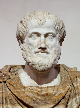
\includegraphics[width=0.5\textwidth]{fig/aristotle}
}

\frame{\frametitle{}
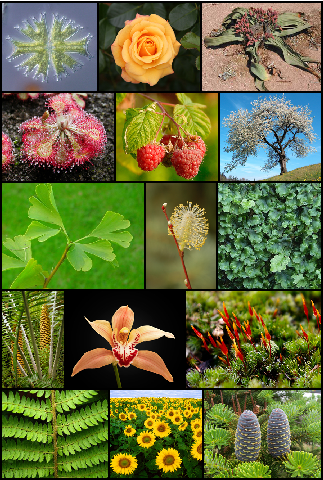
\includegraphics[width=0.5\textwidth]{fig/plant}
}

\frame{\frametitle{}
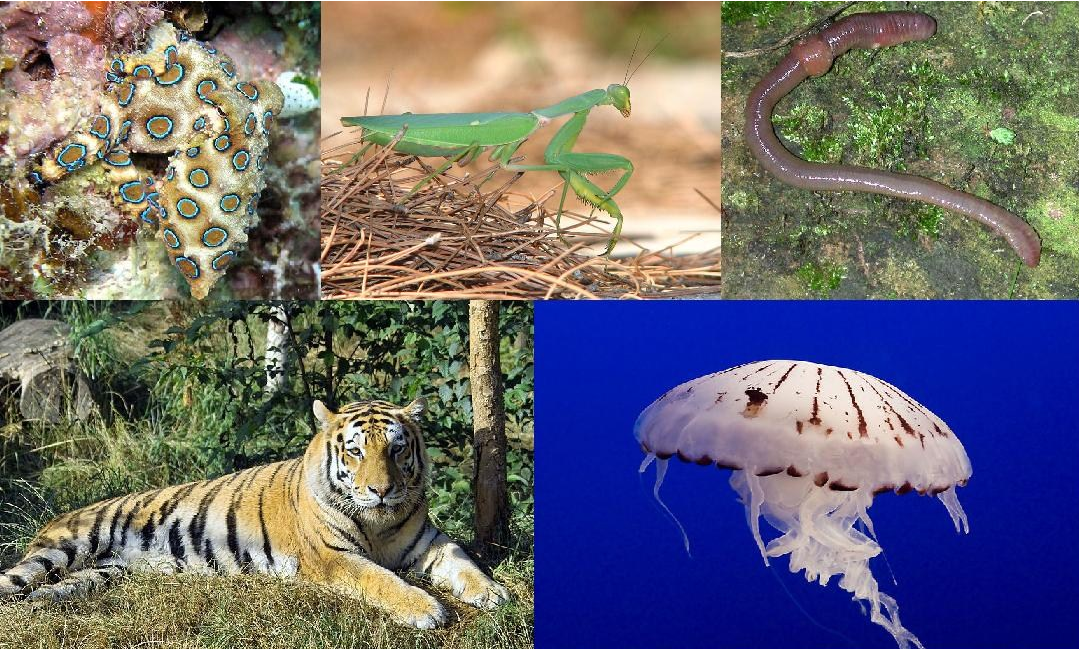
\includegraphics[width=0.5\textwidth]{fig/animal}
}


\frame{\frametitle{}
\centering
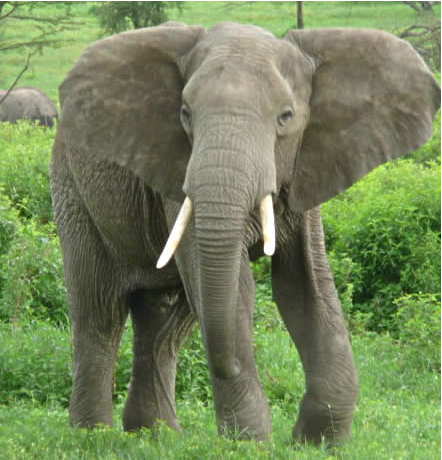
\includegraphics[height=3cm]{fig/elephant}
\pause
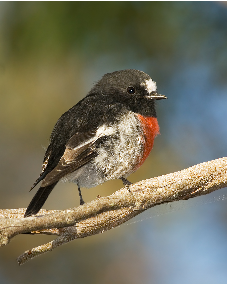
\includegraphics[height=3cm]{fig/bird}
\pause
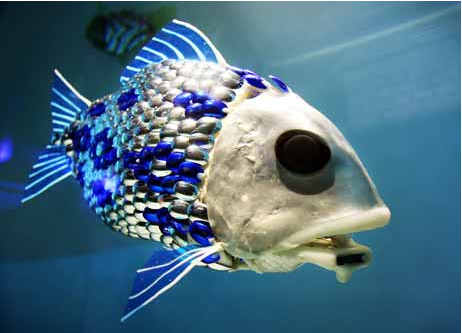
\includegraphics[height=3cm]{fig/fish}
}

\frame{\frametitle{Avicenna}
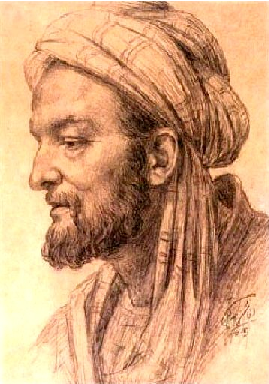
\includegraphics[width=0.5\textwidth]{fig/avicenna}
}


\frame{\frametitle{Mendeleev}
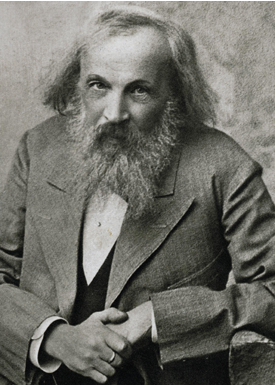
\includegraphics[height=4cm]{fig/mendeleev}
\pause
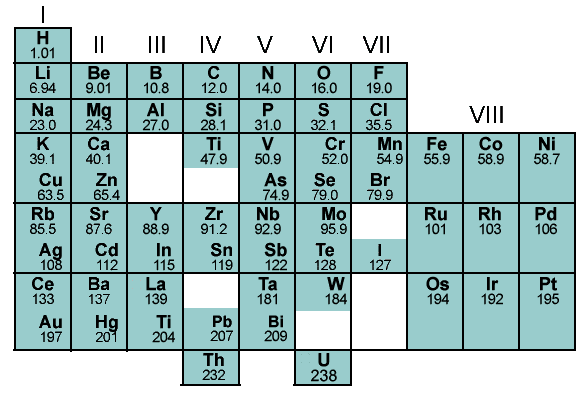
\includegraphics[height=4cm]{fig/periodic1}
}

\frame{\frametitle{}
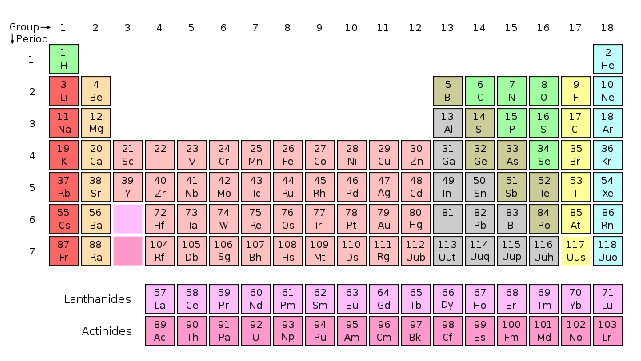
\includegraphics[width=0.9\textwidth]{fig/periodic2}
}


\frame{\frametitle{}
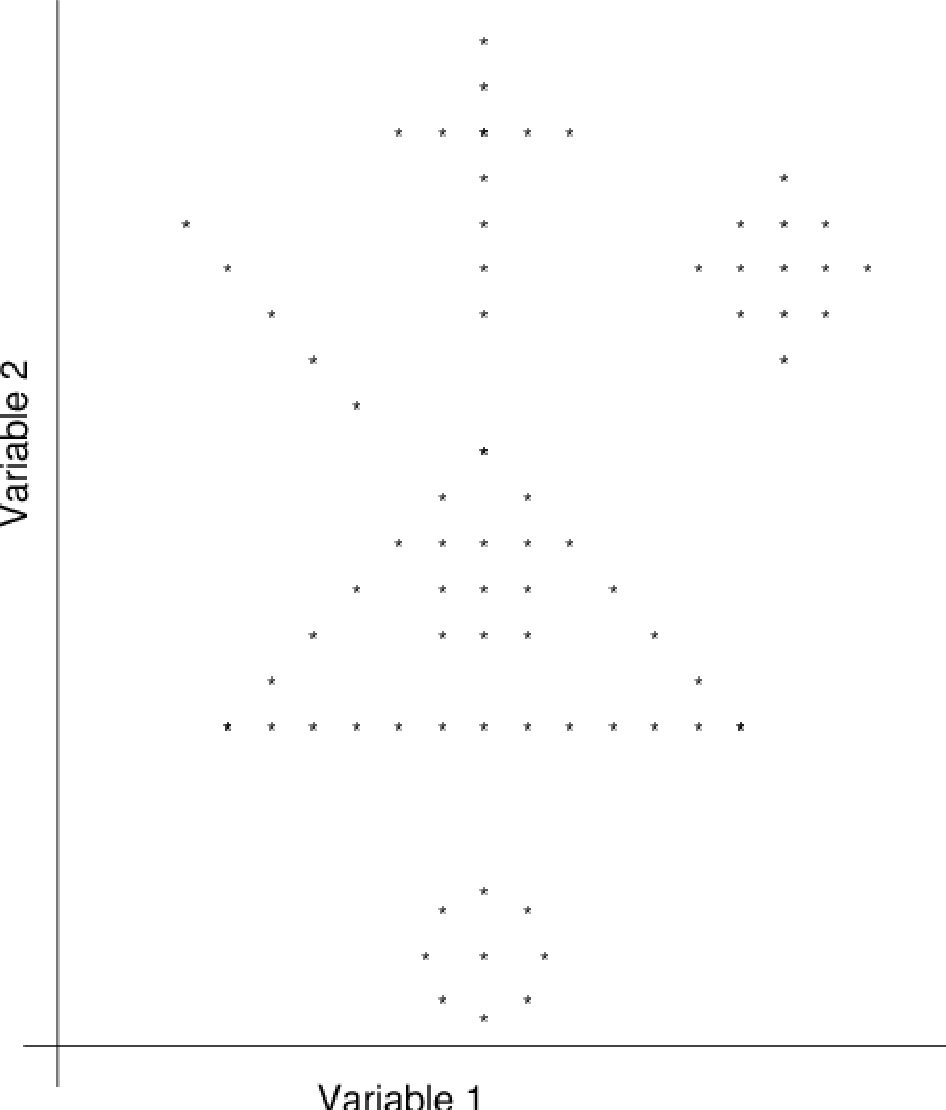
\includegraphics[width=0.5\textwidth]{fig/artificial01}
}

\frame{\frametitle{}
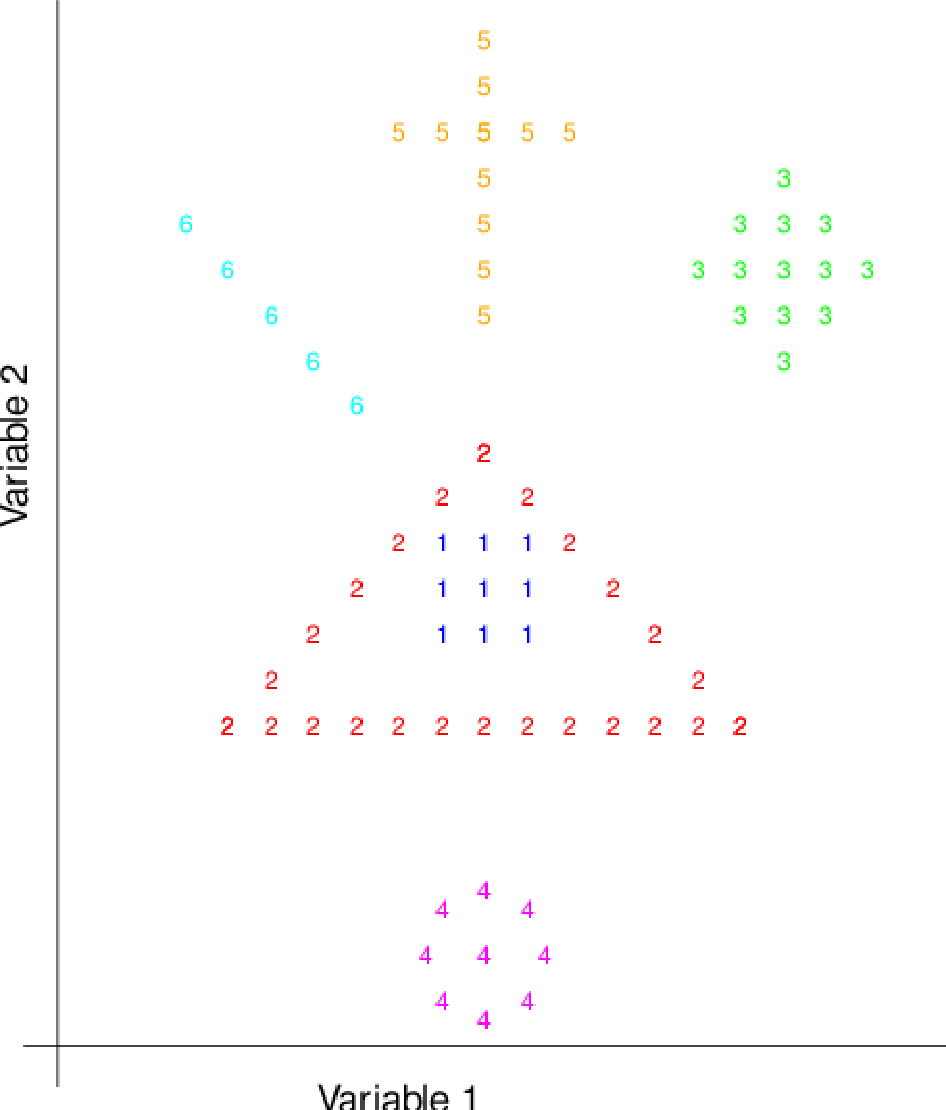
\includegraphics[width=0.5\textwidth]{fig/artificial02}
}


\section{K-Means}

 \frame{\frametitle{Initial 1}
 \centering
 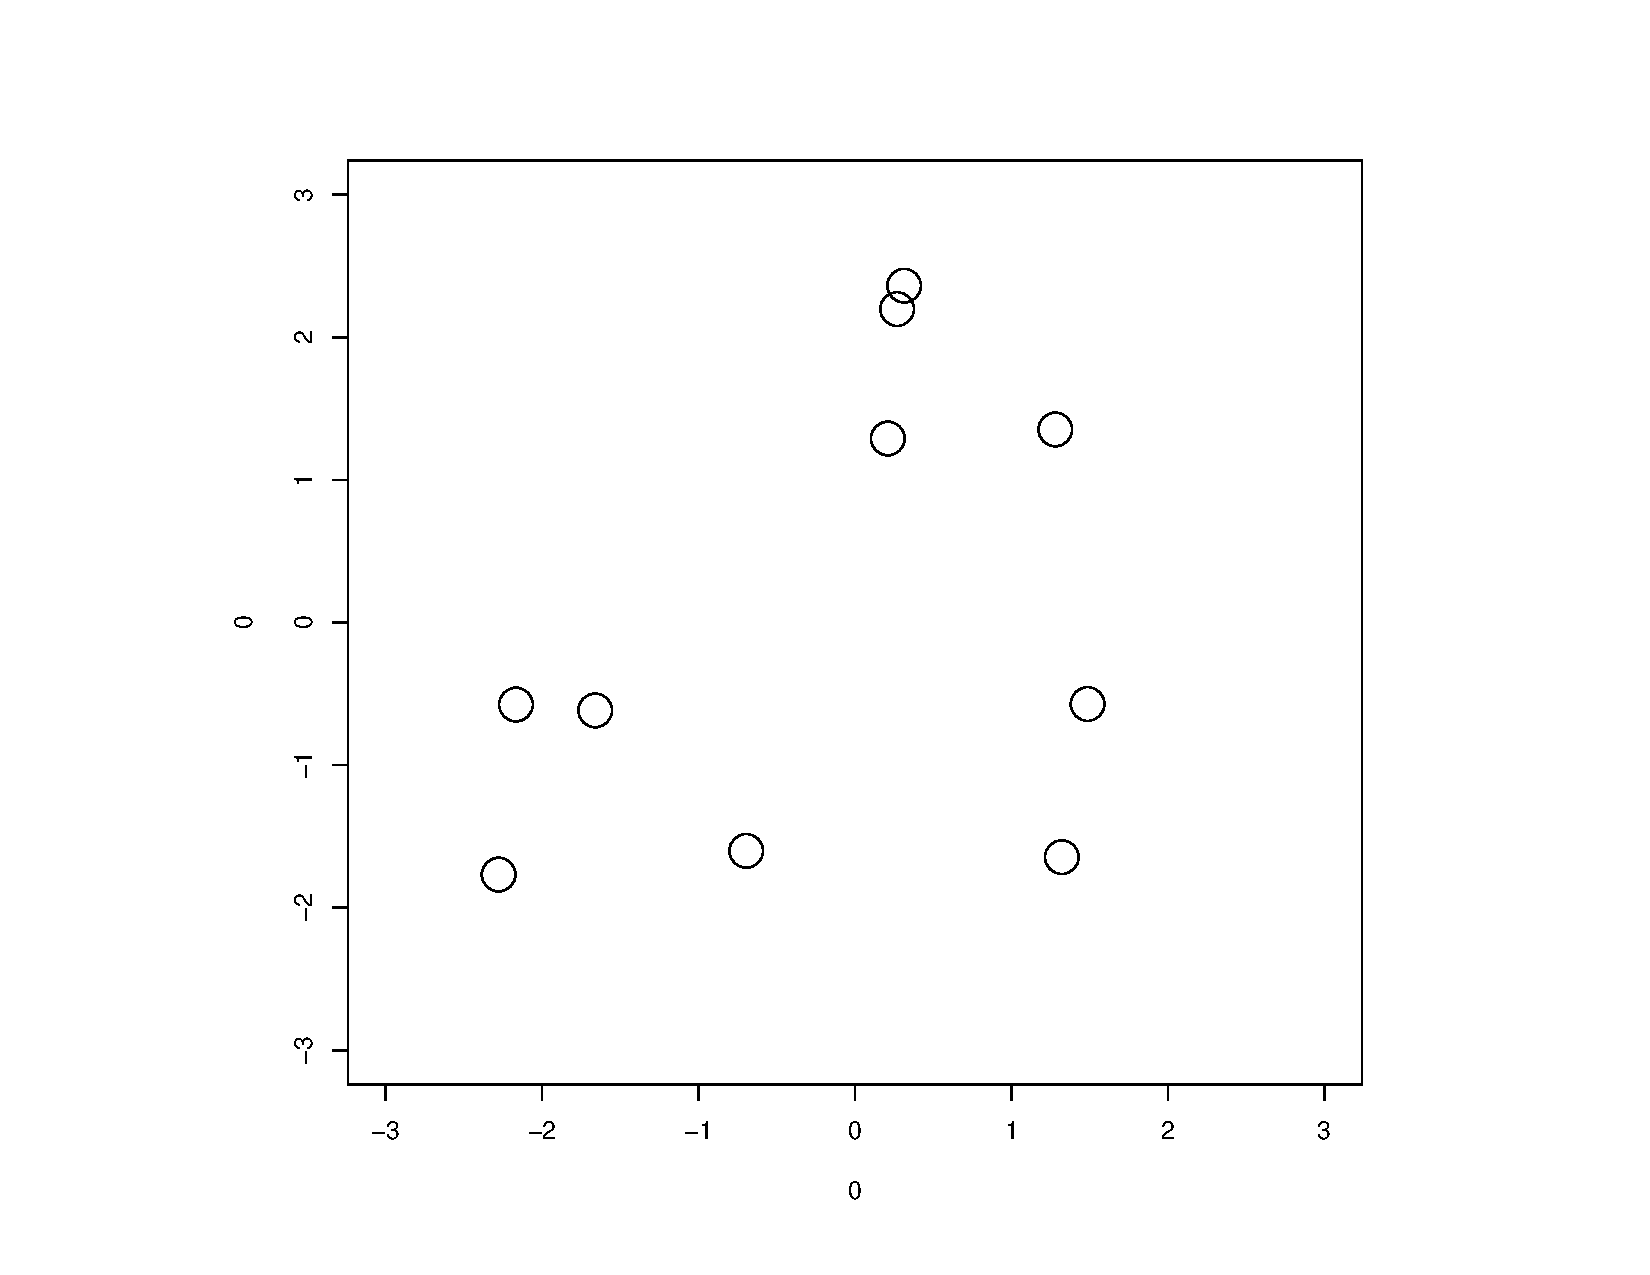
\includegraphics[width=0.7\textwidth]{fig//kmeans101}
 }
 \frame{\frametitle{}
 \centering
 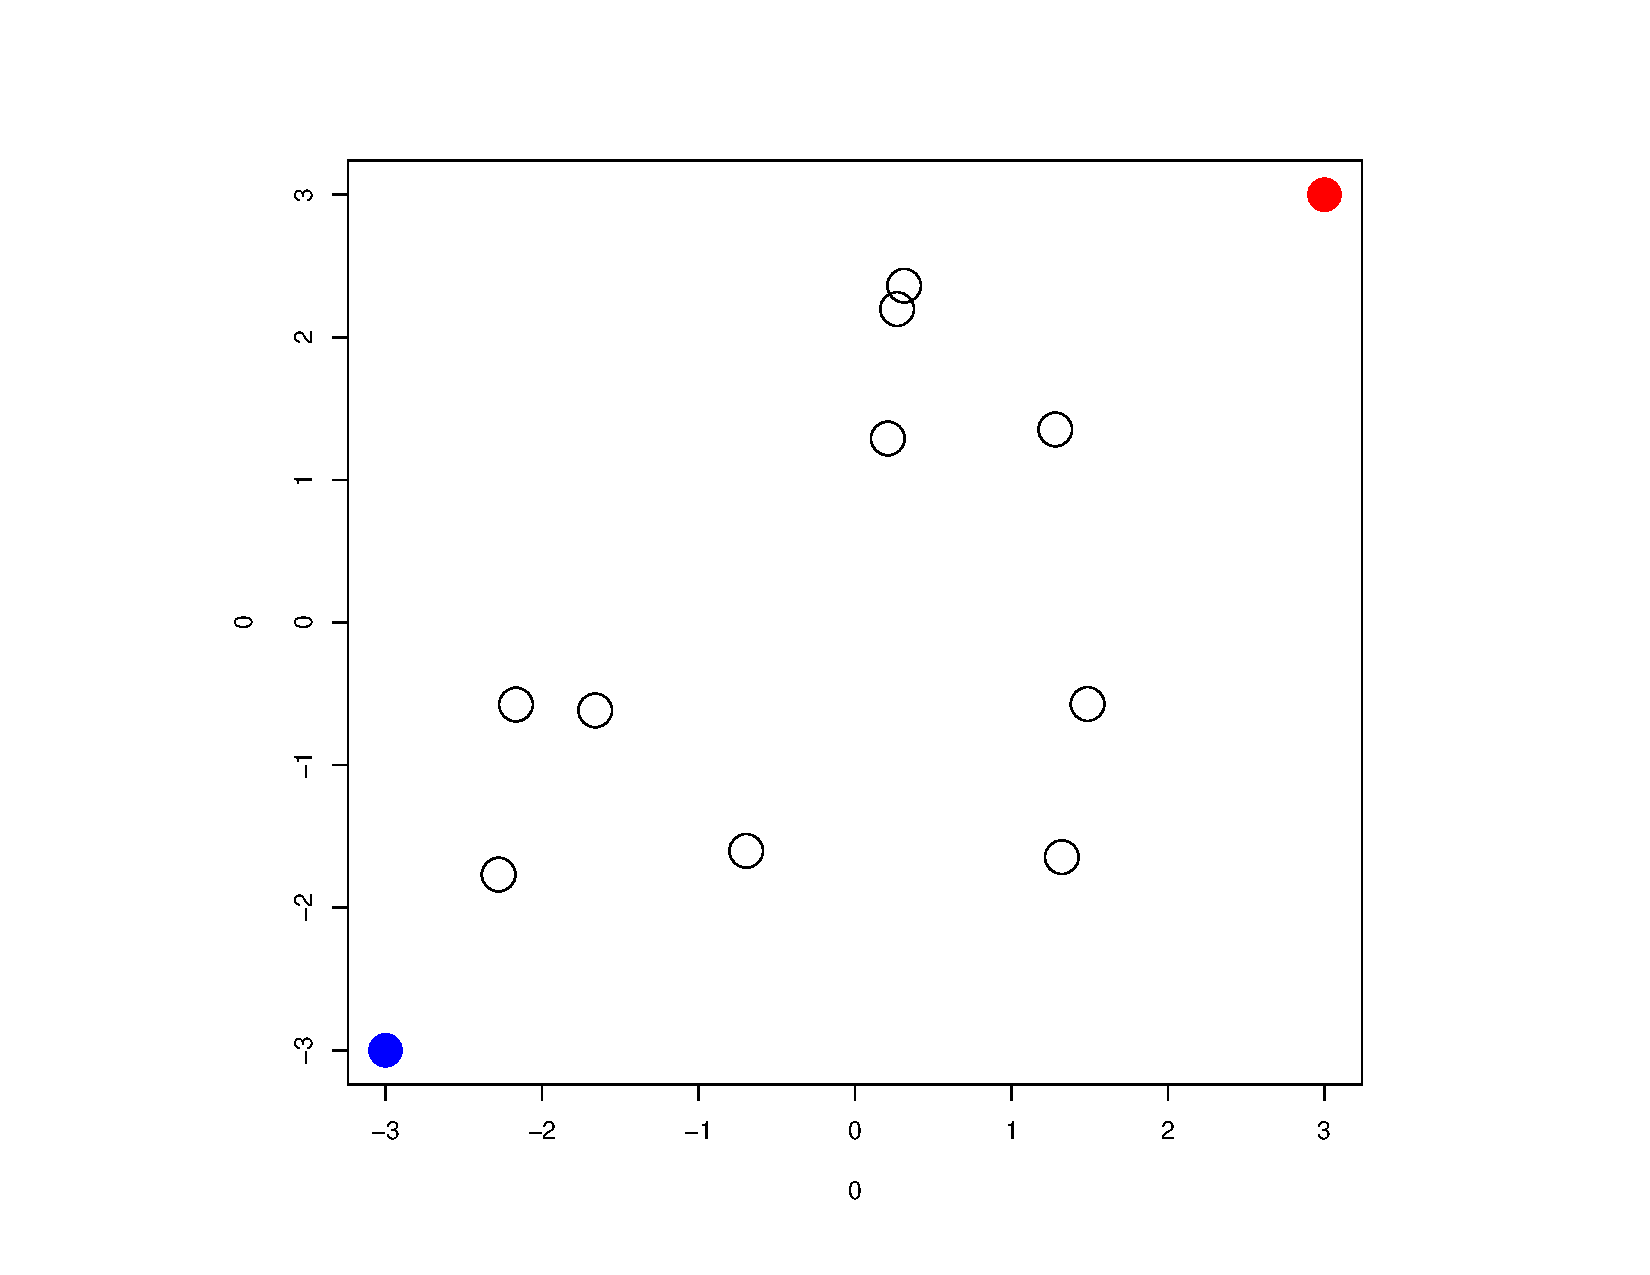
\includegraphics[width=0.7\textwidth ]{fig//kmeans102}
 }
 \frame{\frametitle{}
 \centering
 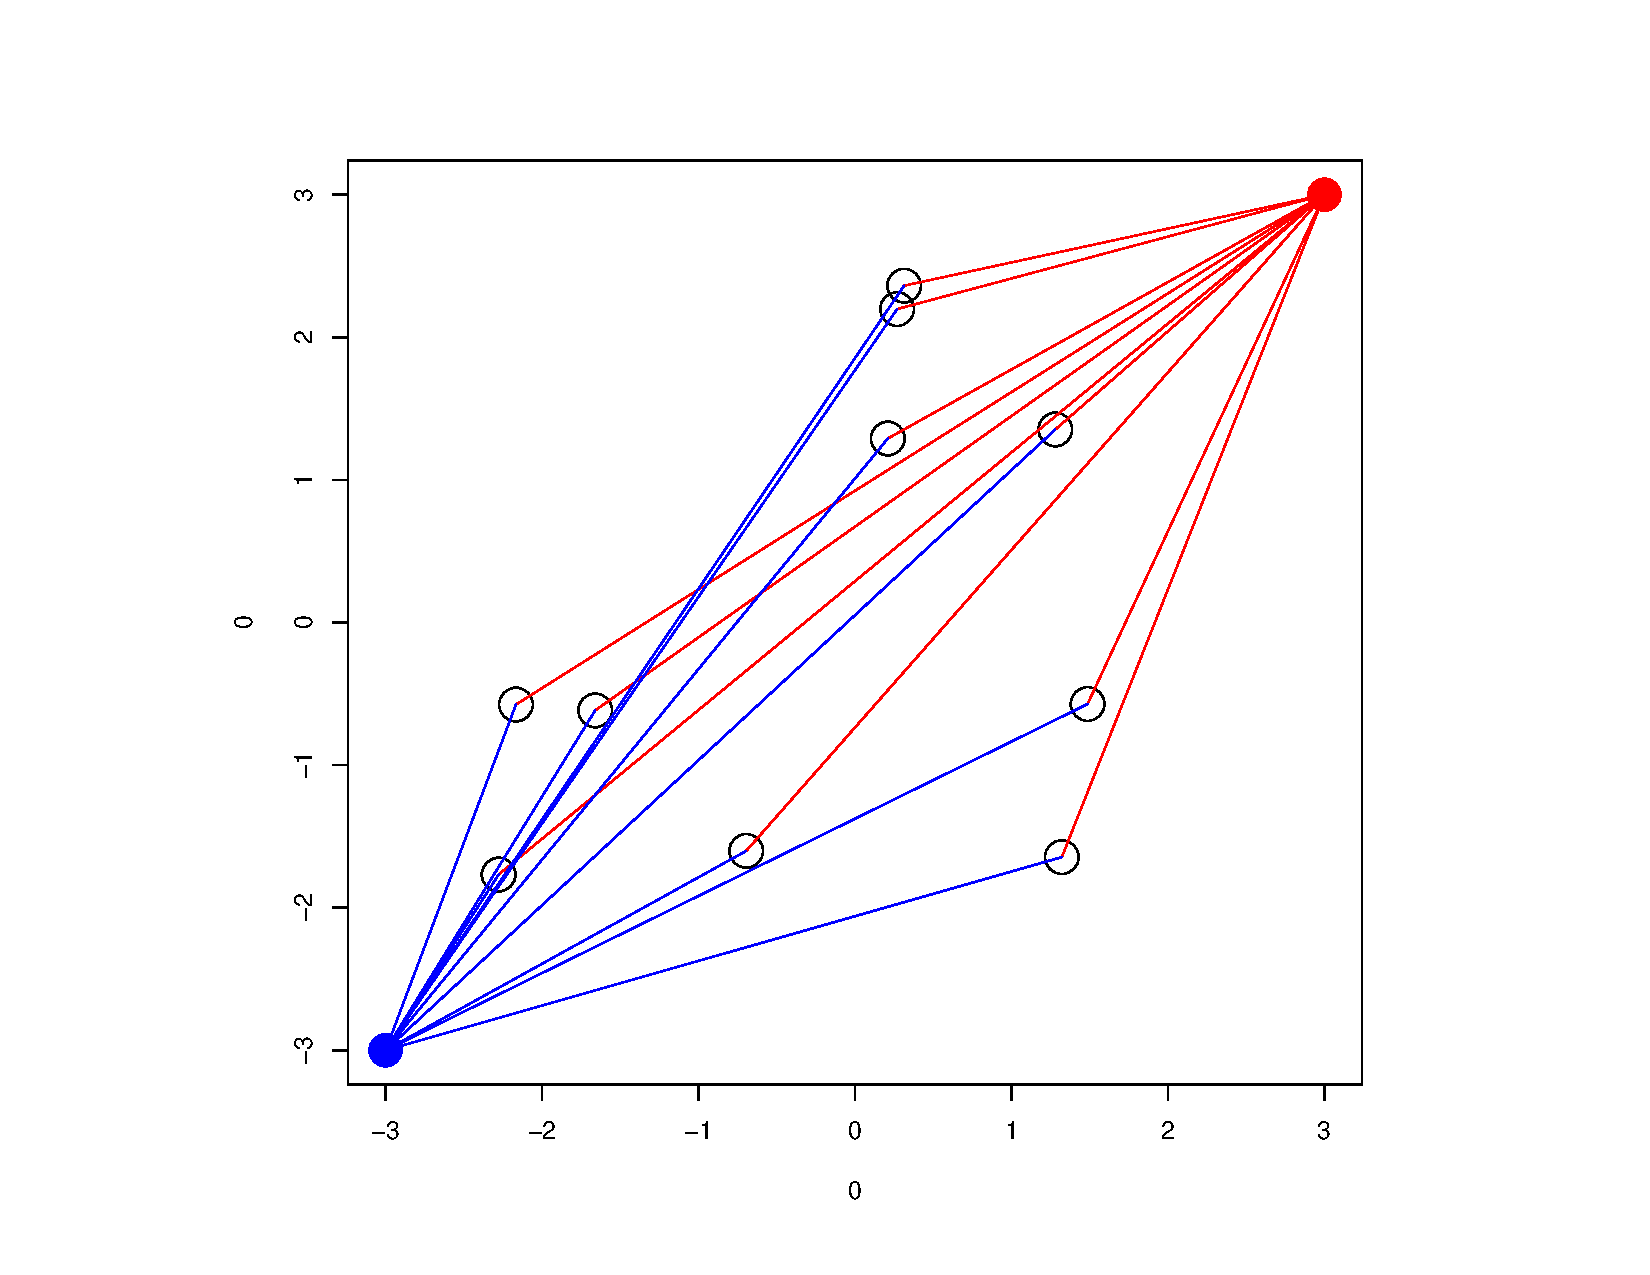
\includegraphics[width=0.7\textwidth ]{fig//kmeans103}
 }
 \frame{\frametitle{}
 \centering
 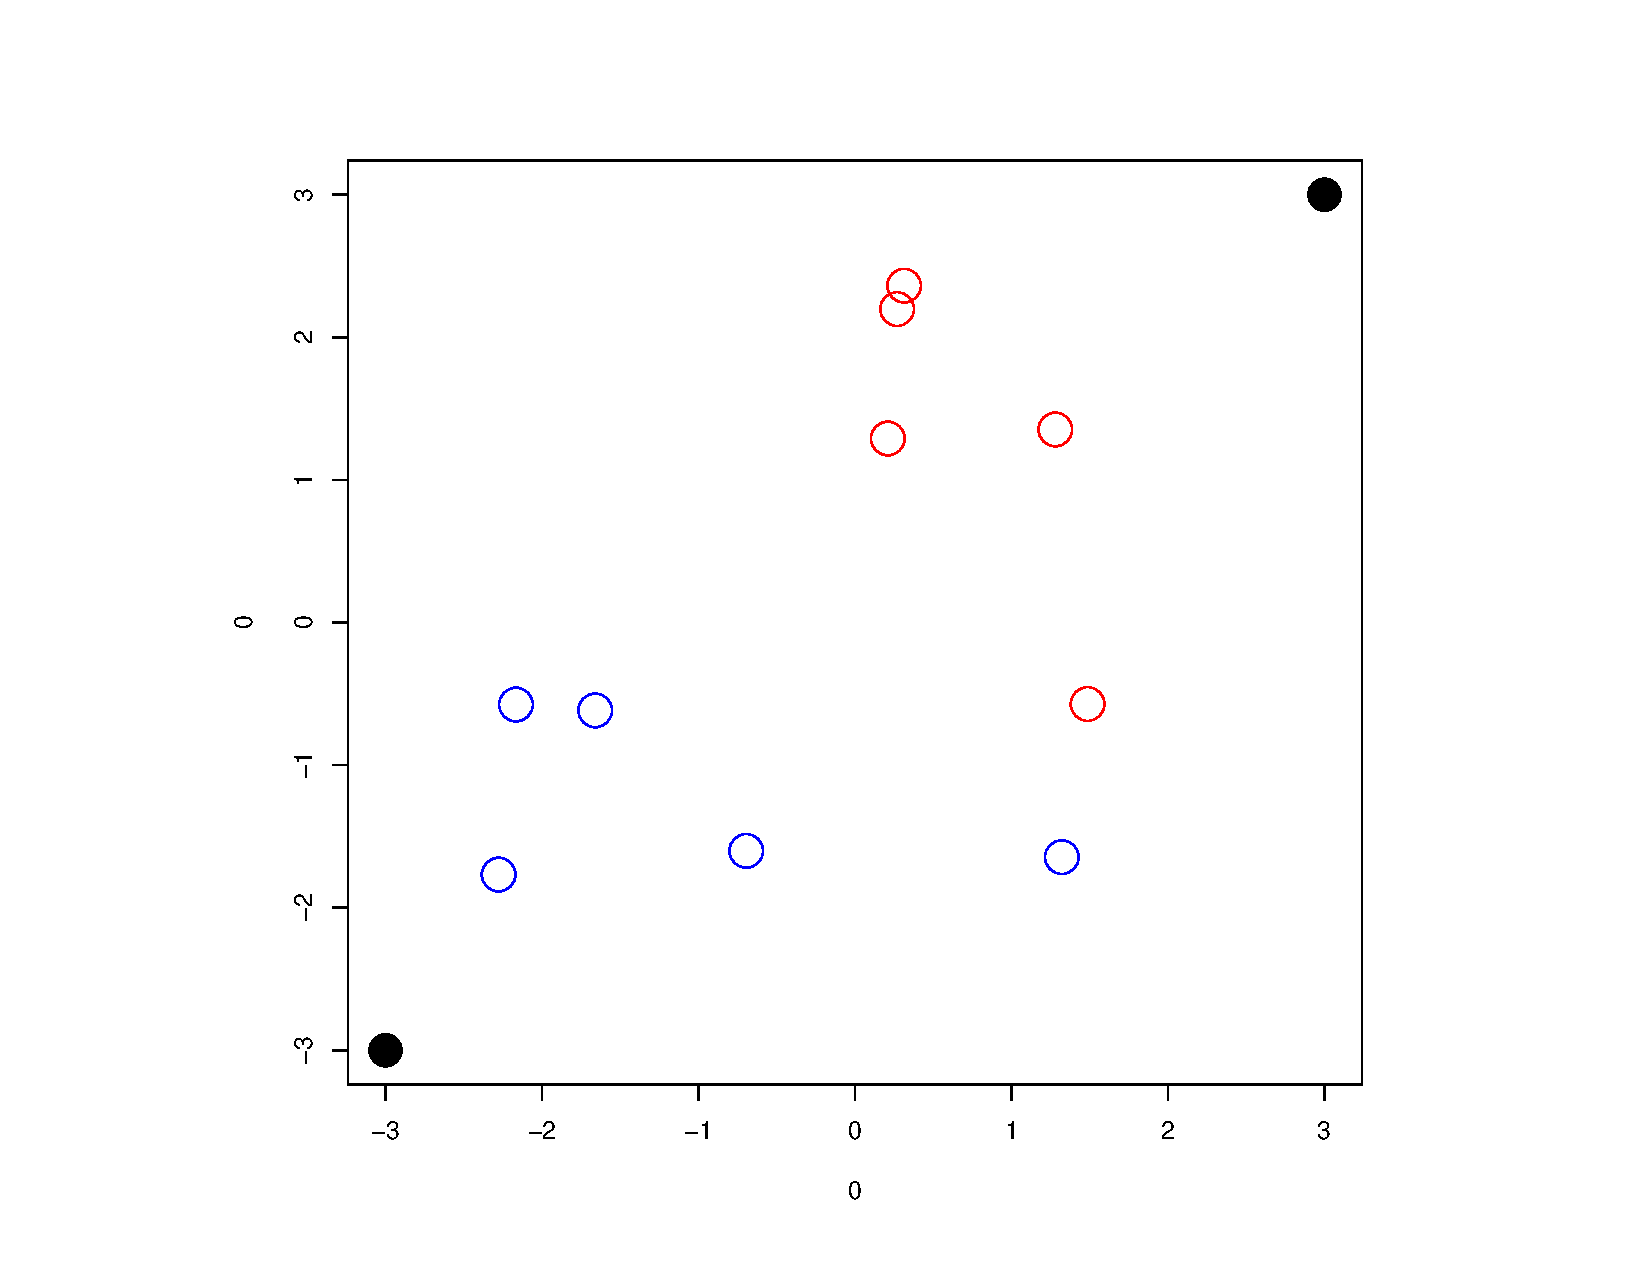
\includegraphics[width=0.7\textwidth ]{fig//kmeans104}
 }
 \frame{\frametitle{}
 \centering
 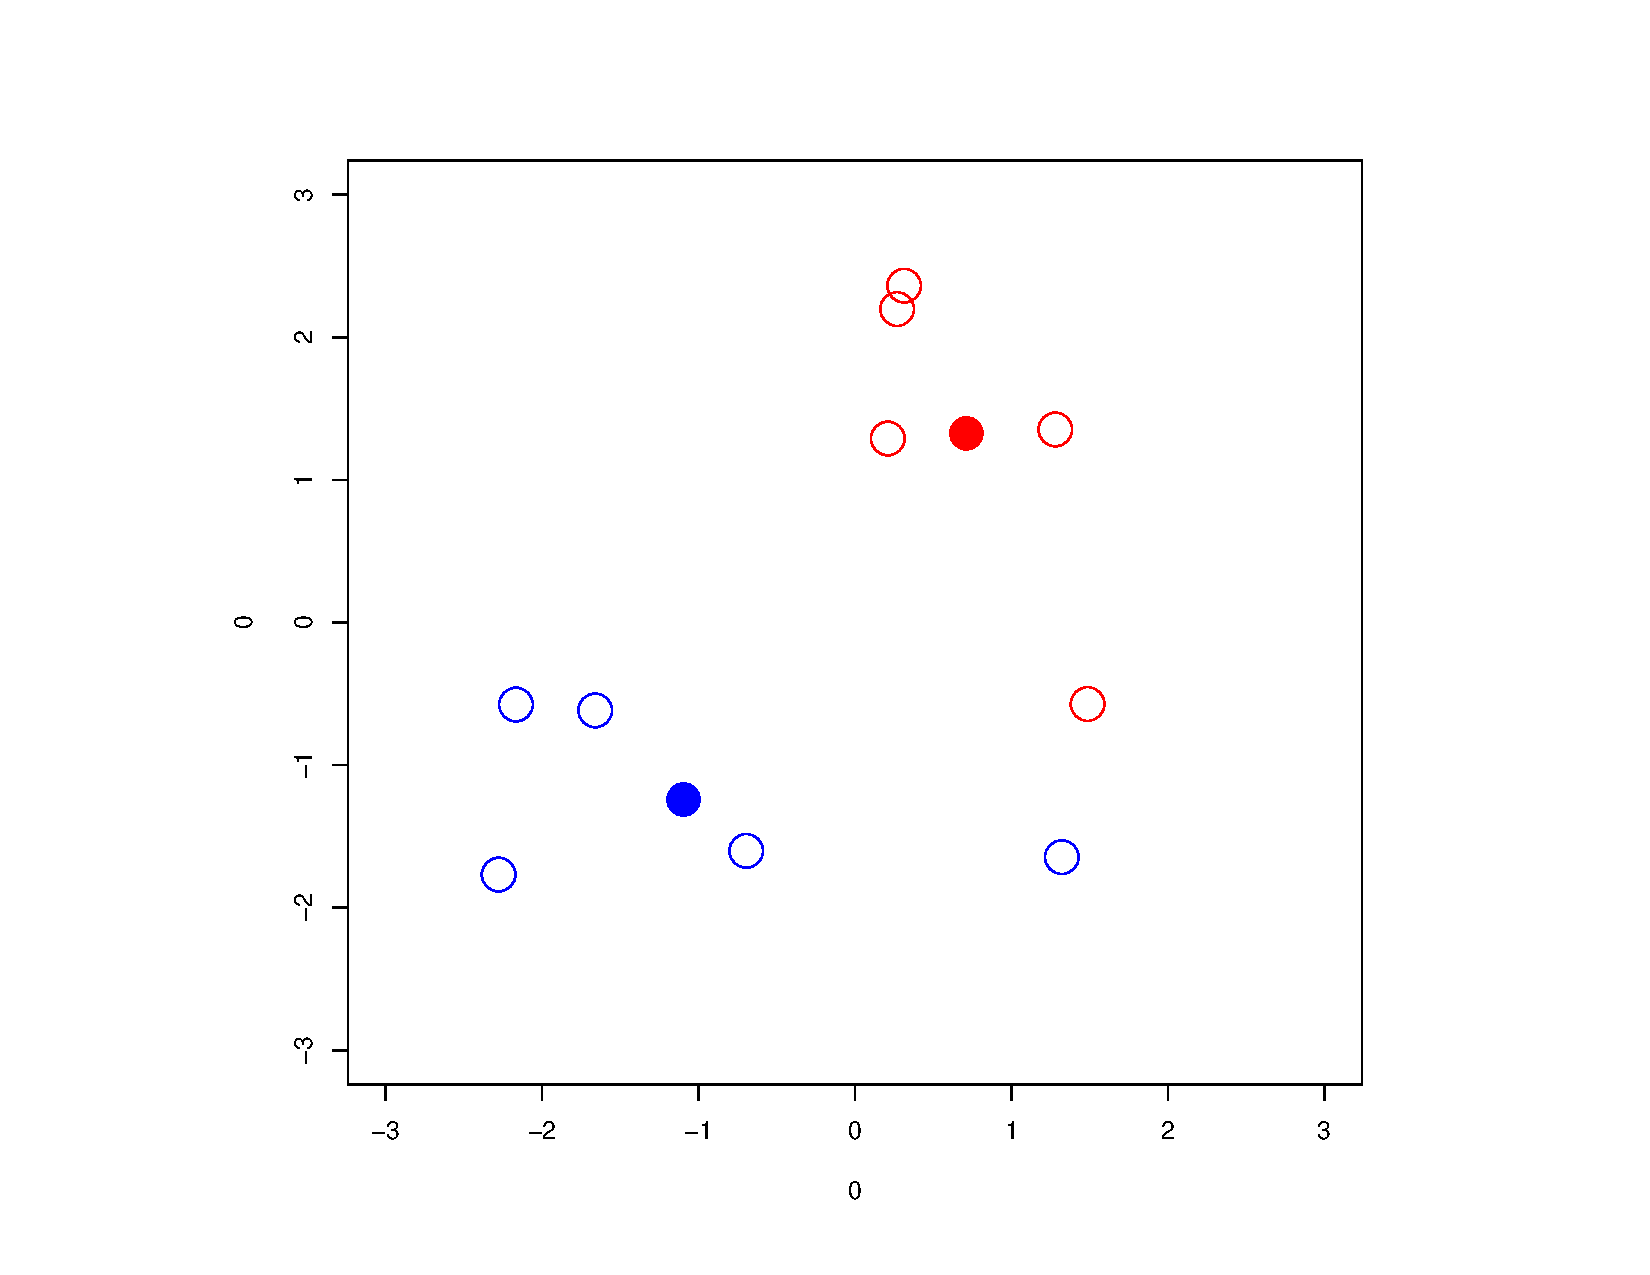
\includegraphics[width=0.7\textwidth ]{fig//kmeans105}
 }
 \frame{\frametitle{}
 \centering
 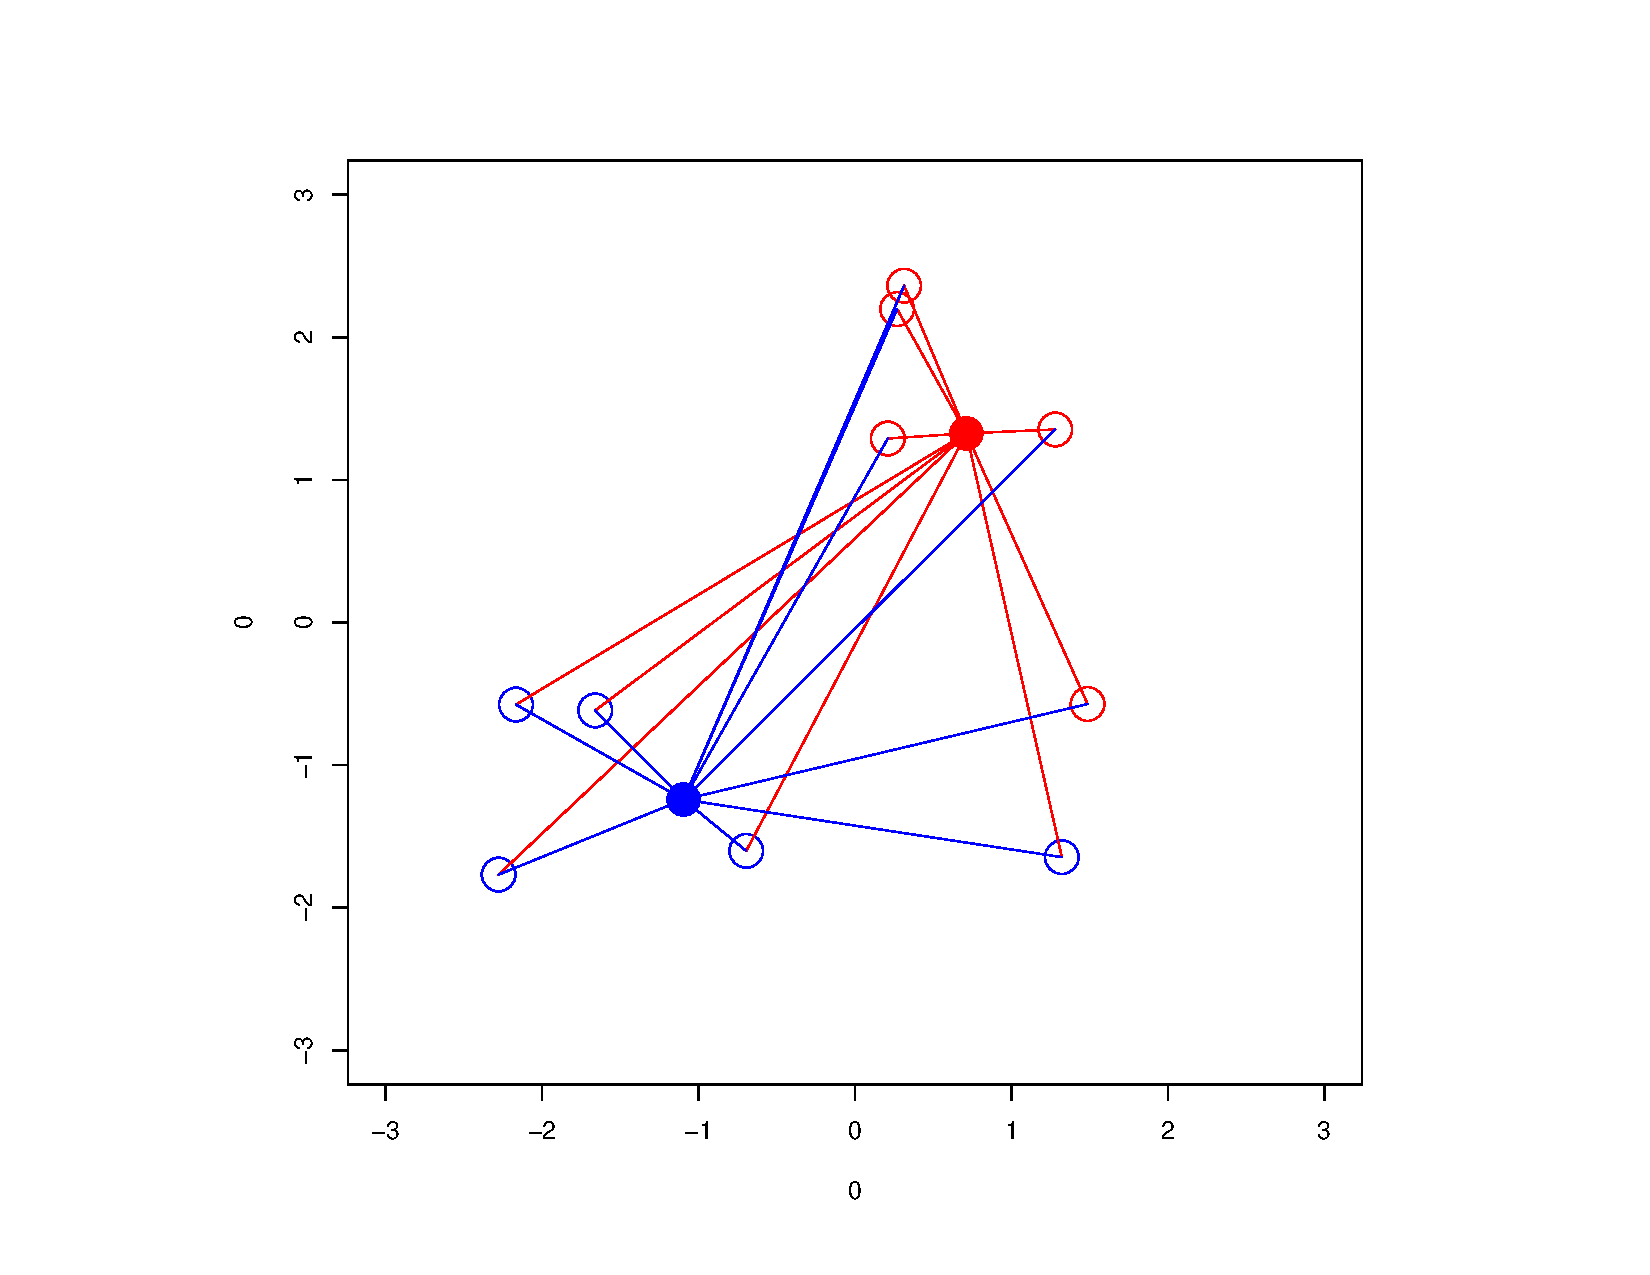
\includegraphics[width=0.7\textwidth ]{fig//kmeans106}
 }
 \frame{\frametitle{}
 \centering
 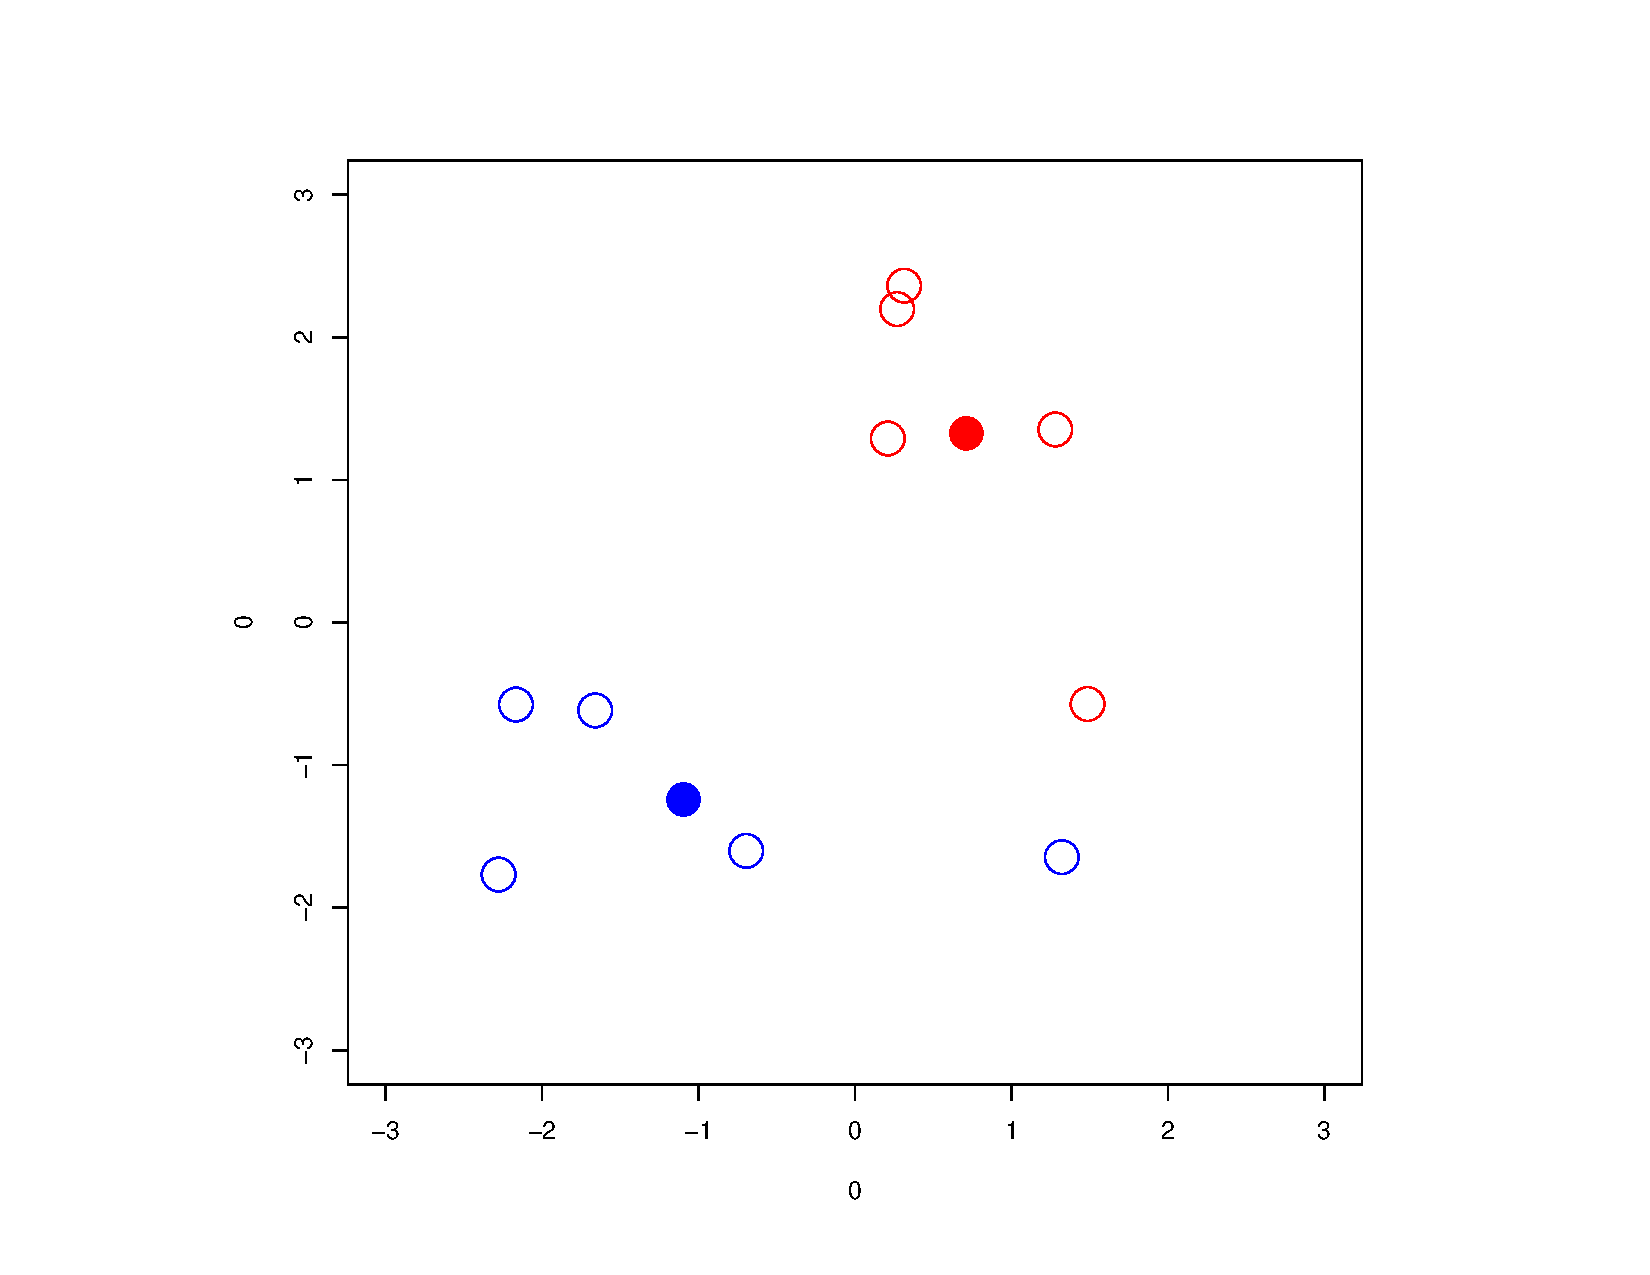
\includegraphics[width=0.7\textwidth ]{fig//kmeans105}
 }
 
 \frame{\frametitle{Initial 2}
 \centering
 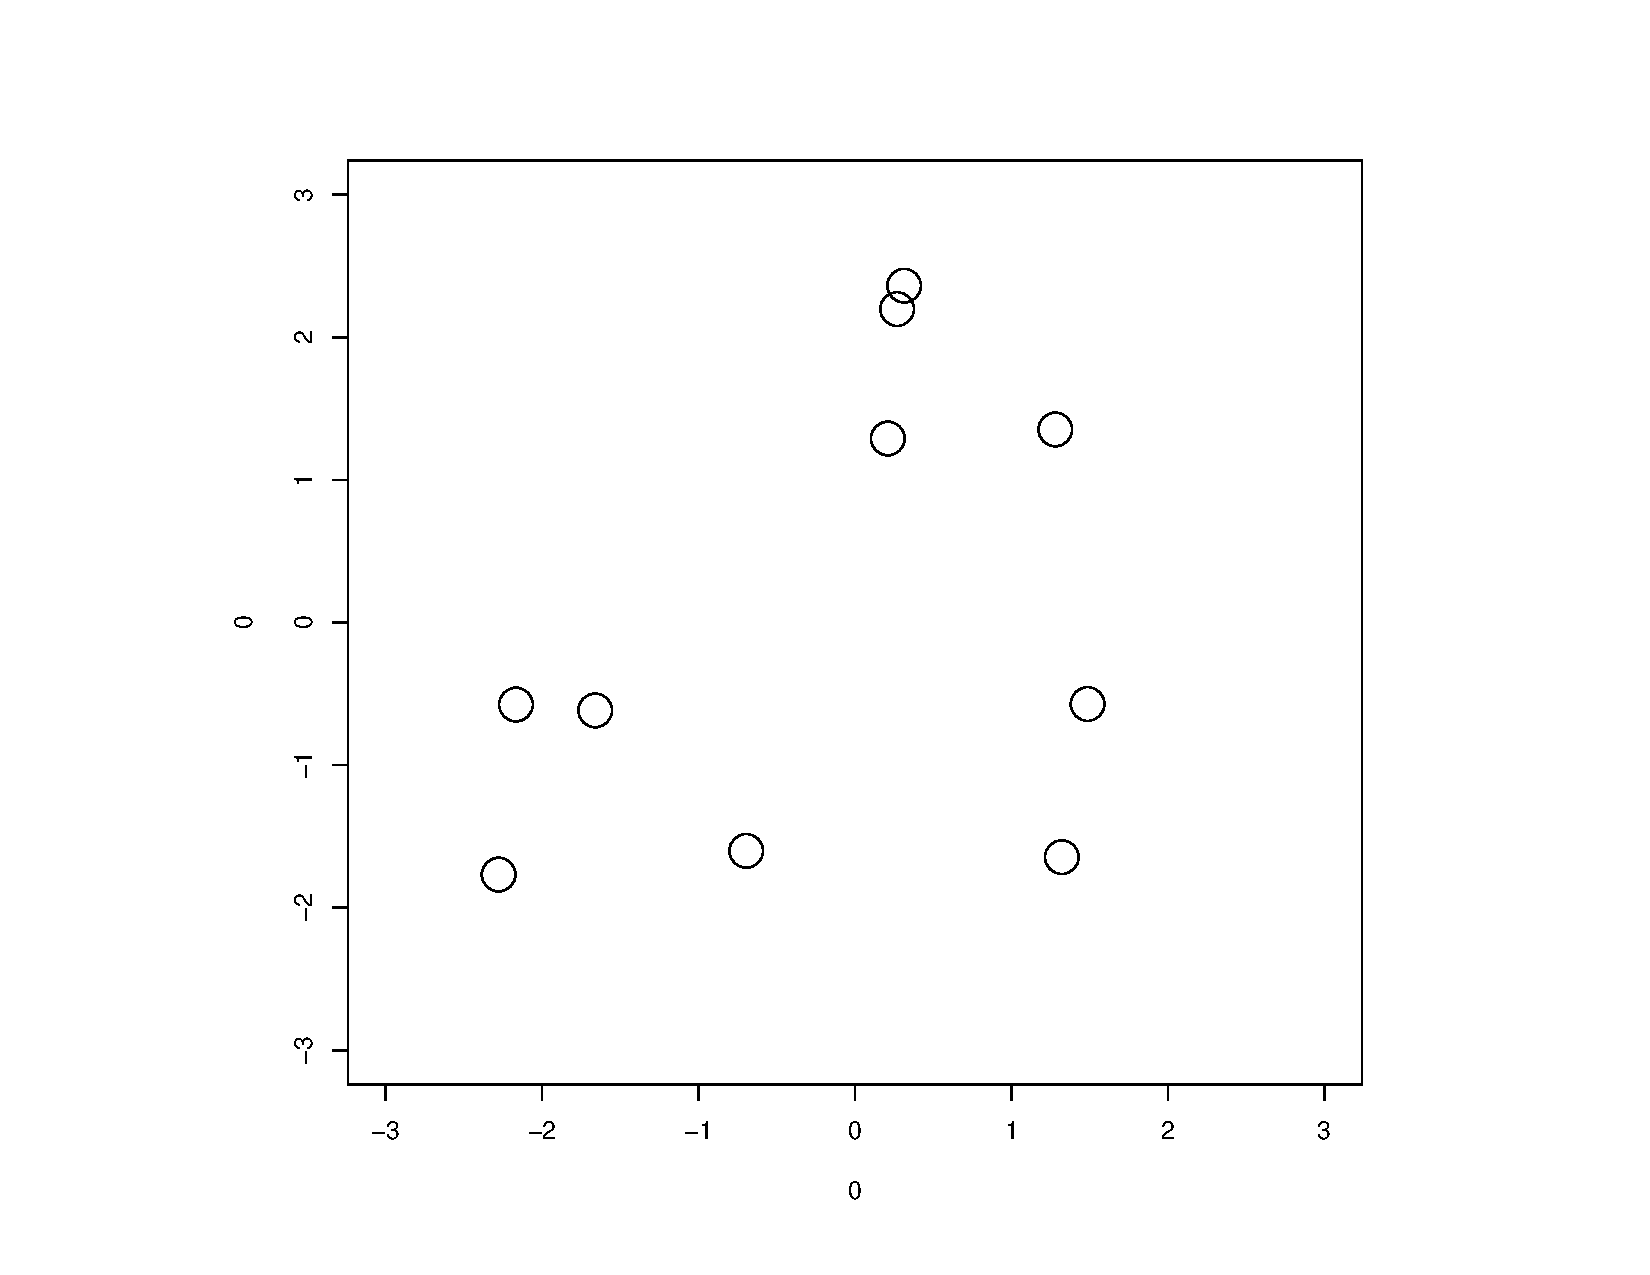
\includegraphics[width=0.7\textwidth ]{fig//kmeans201}
 }
 \frame{\frametitle{}
 \centering
 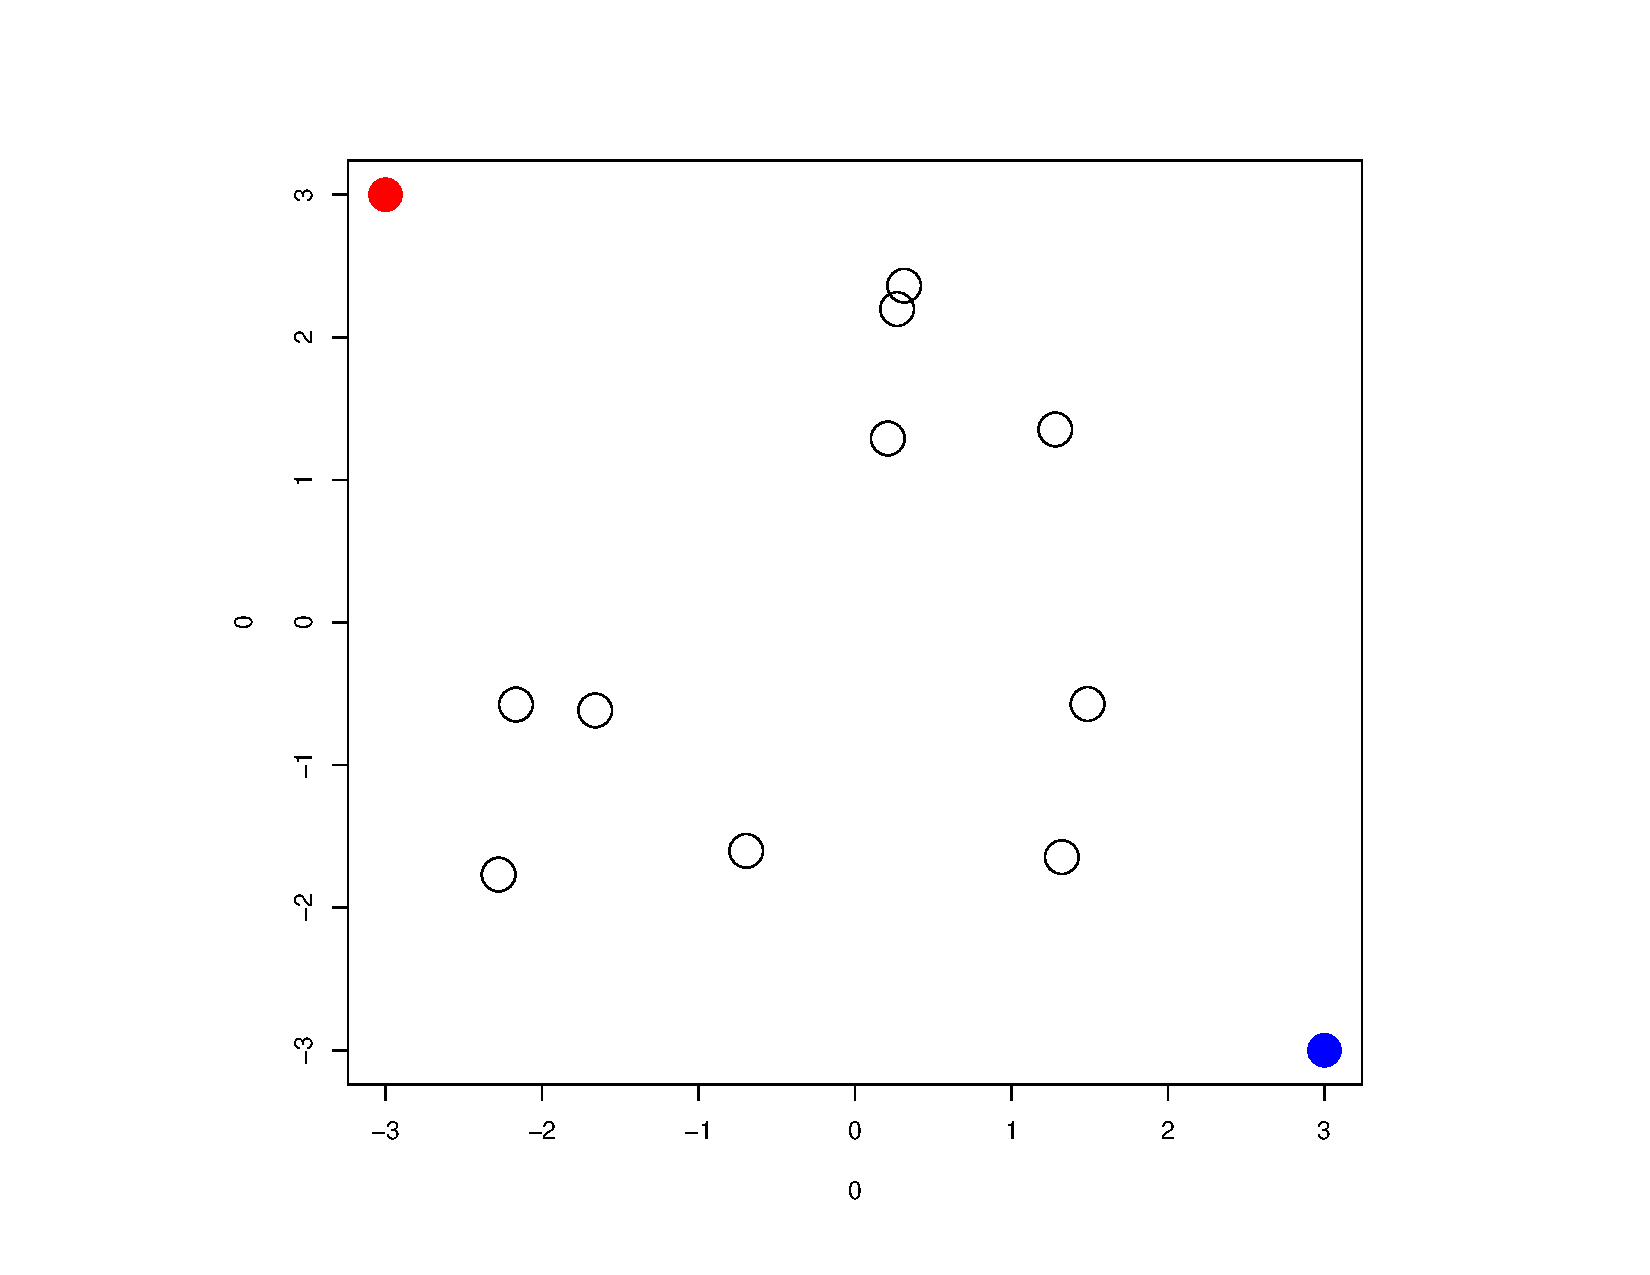
\includegraphics[width=0.7\textwidth ]{fig//kmeans202}
 }
 \frame{\frametitle{}
 \centering
 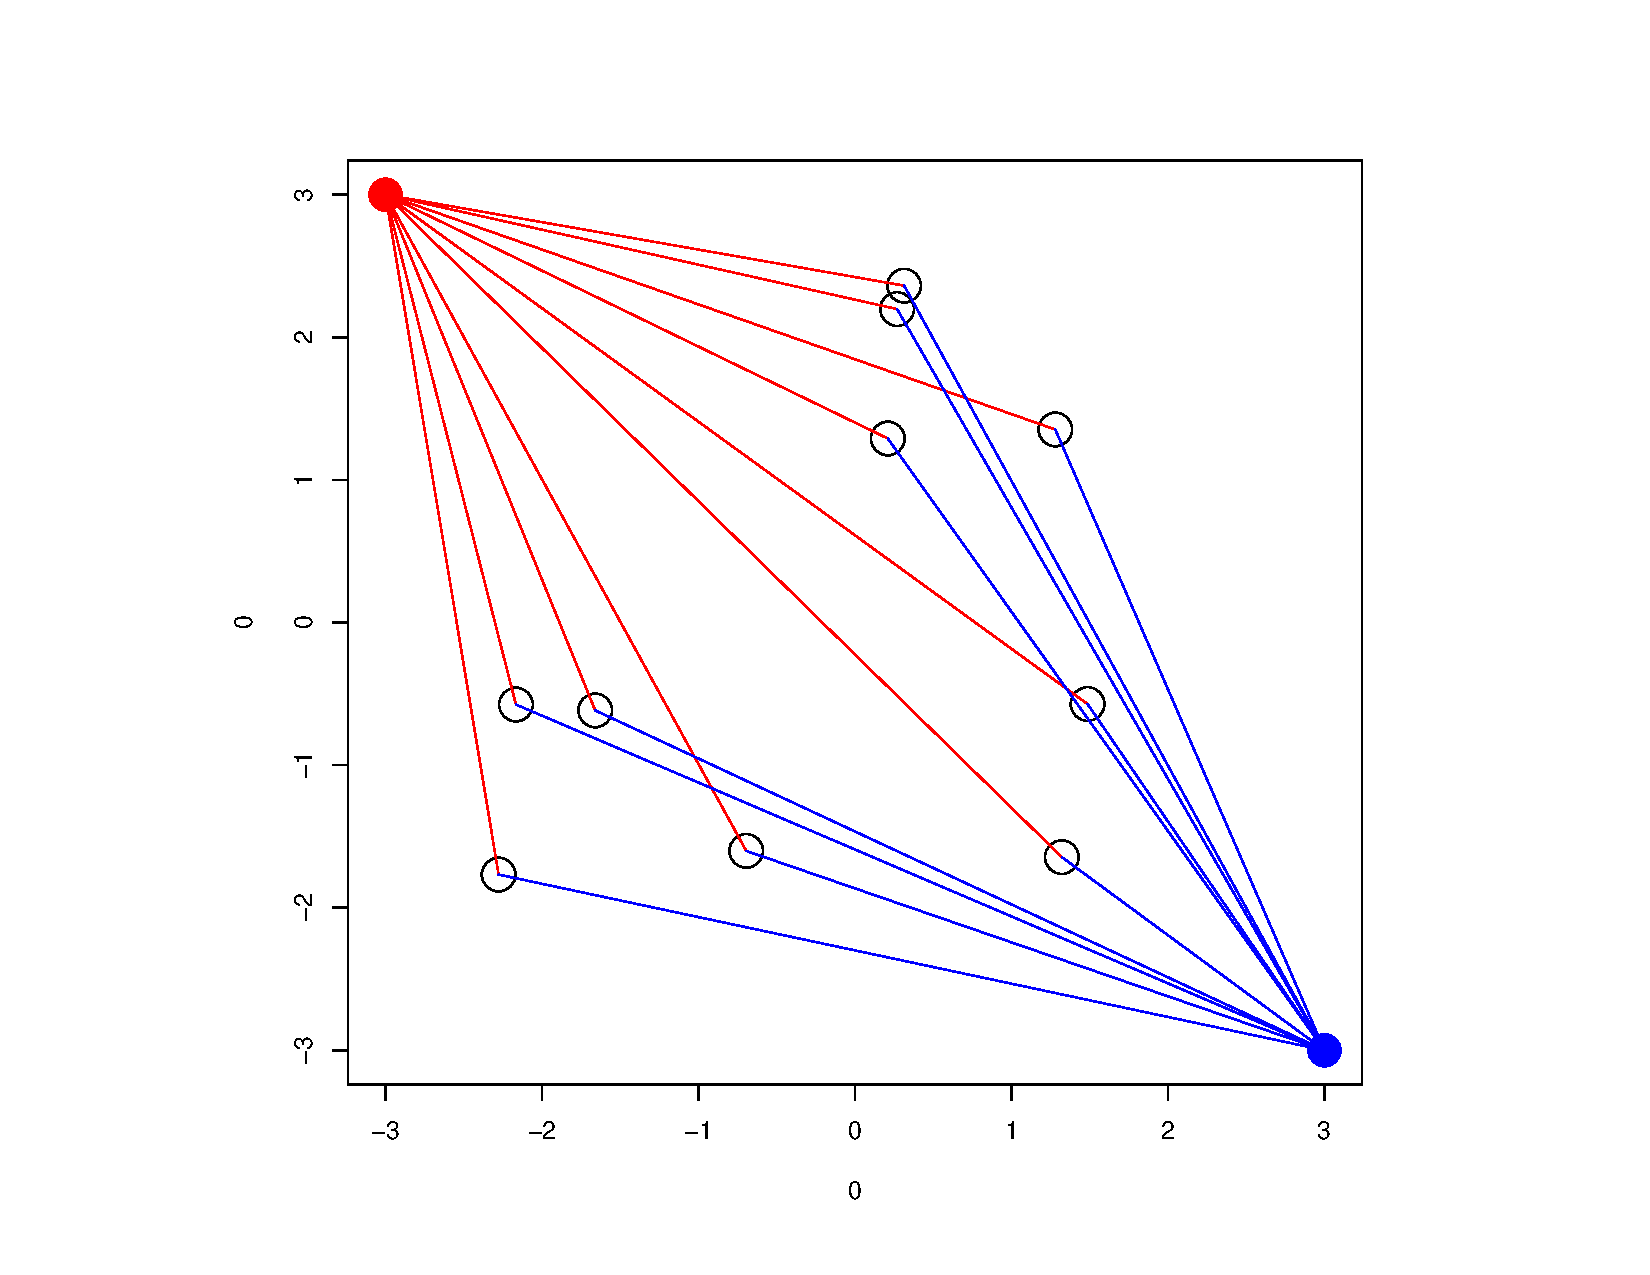
\includegraphics[width=0.7\textwidth ]{fig//kmeans203}
 }
 \frame{\frametitle{}
 \centering
 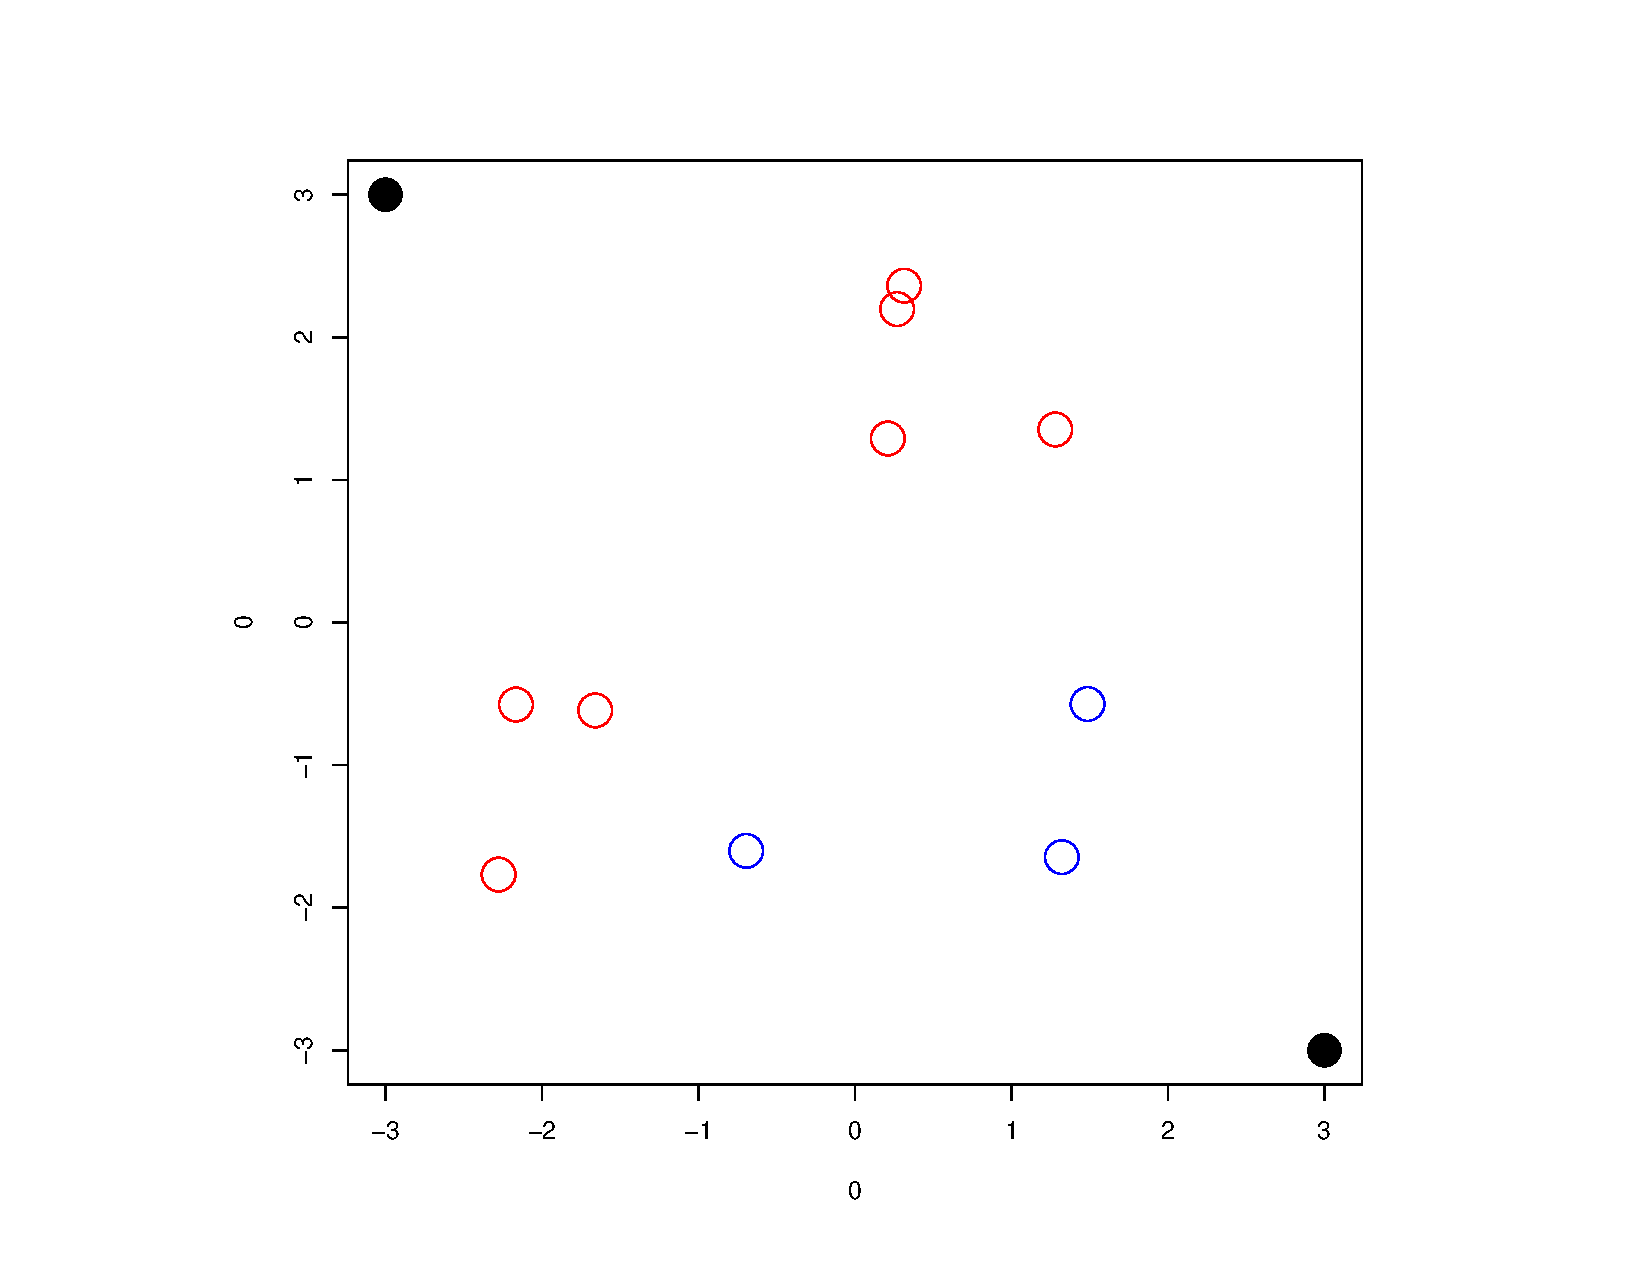
\includegraphics[width=0.7\textwidth ]{fig//kmeans204}
 }
 \frame{\frametitle{}
 \centering
 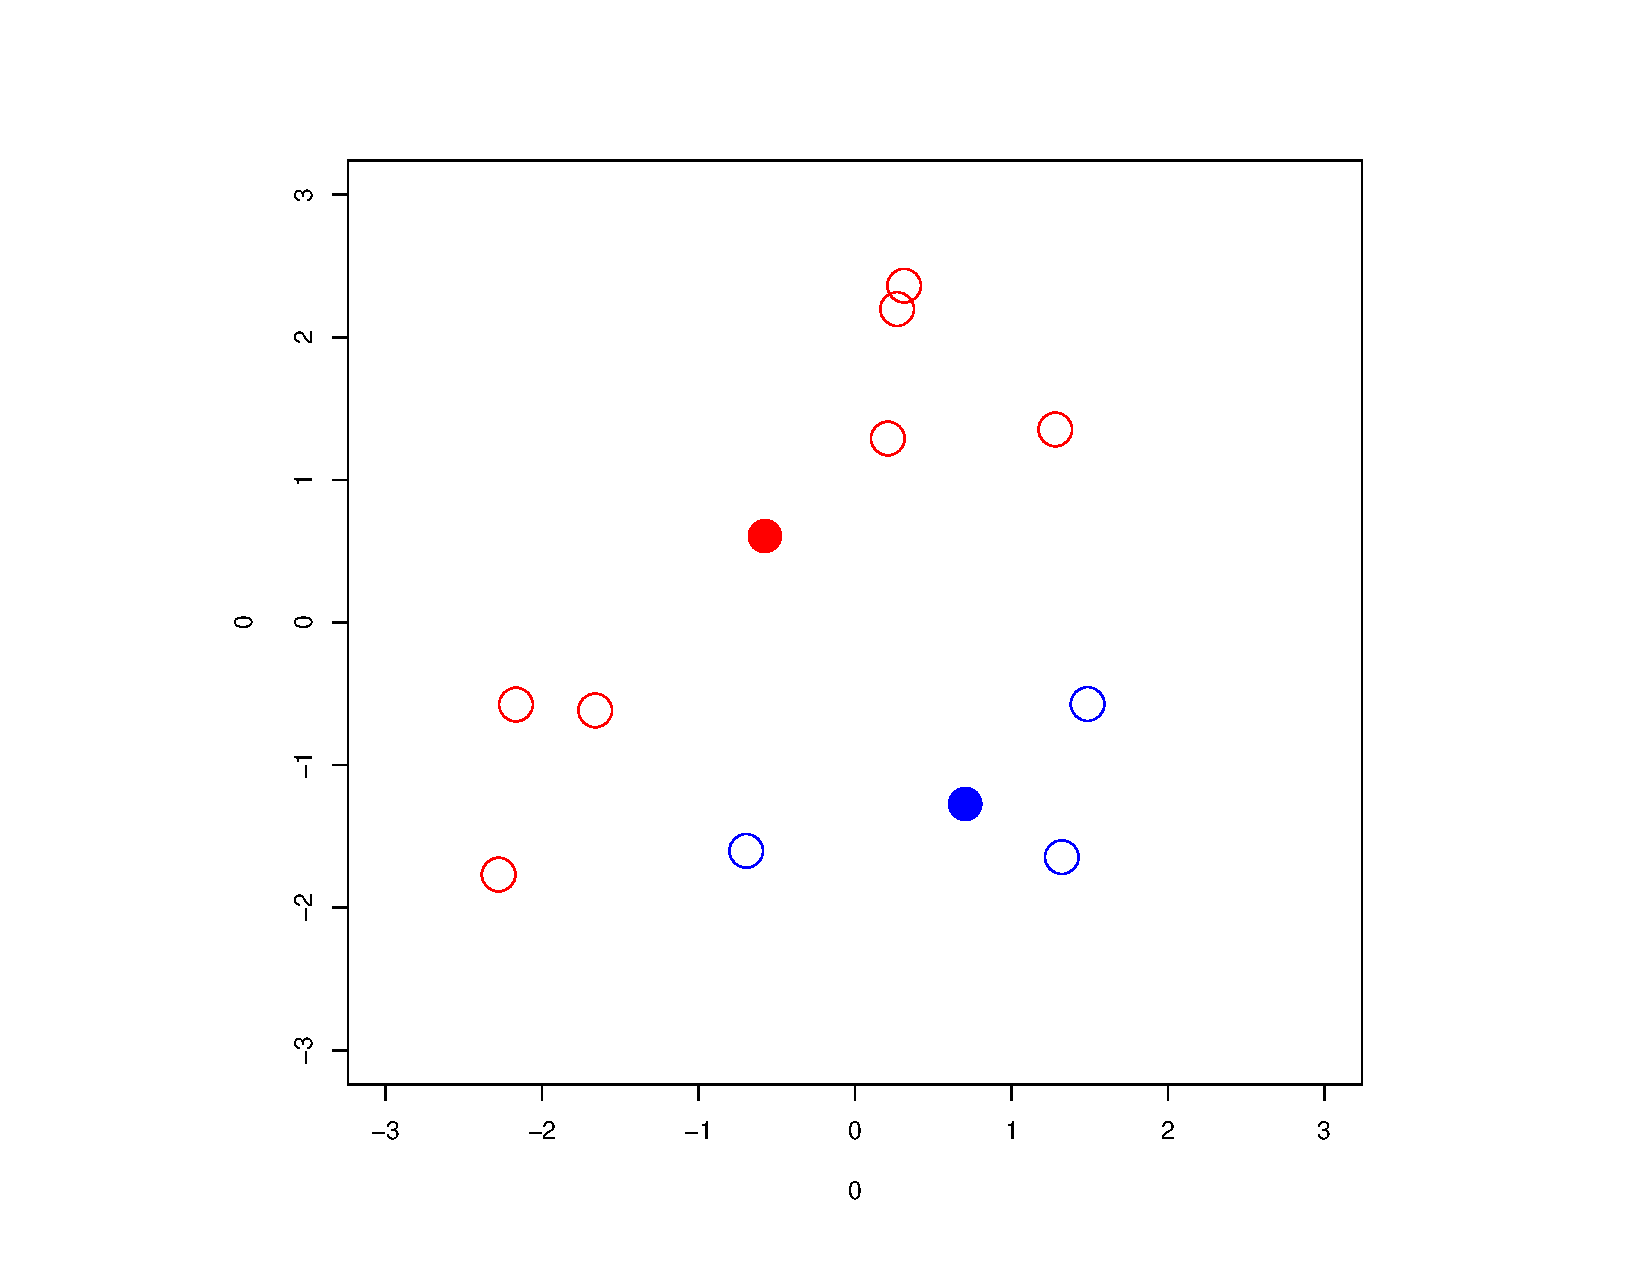
\includegraphics[width=0.7\textwidth ]{fig//kmeans205}
 }
 \frame{\frametitle{}
 \centering
 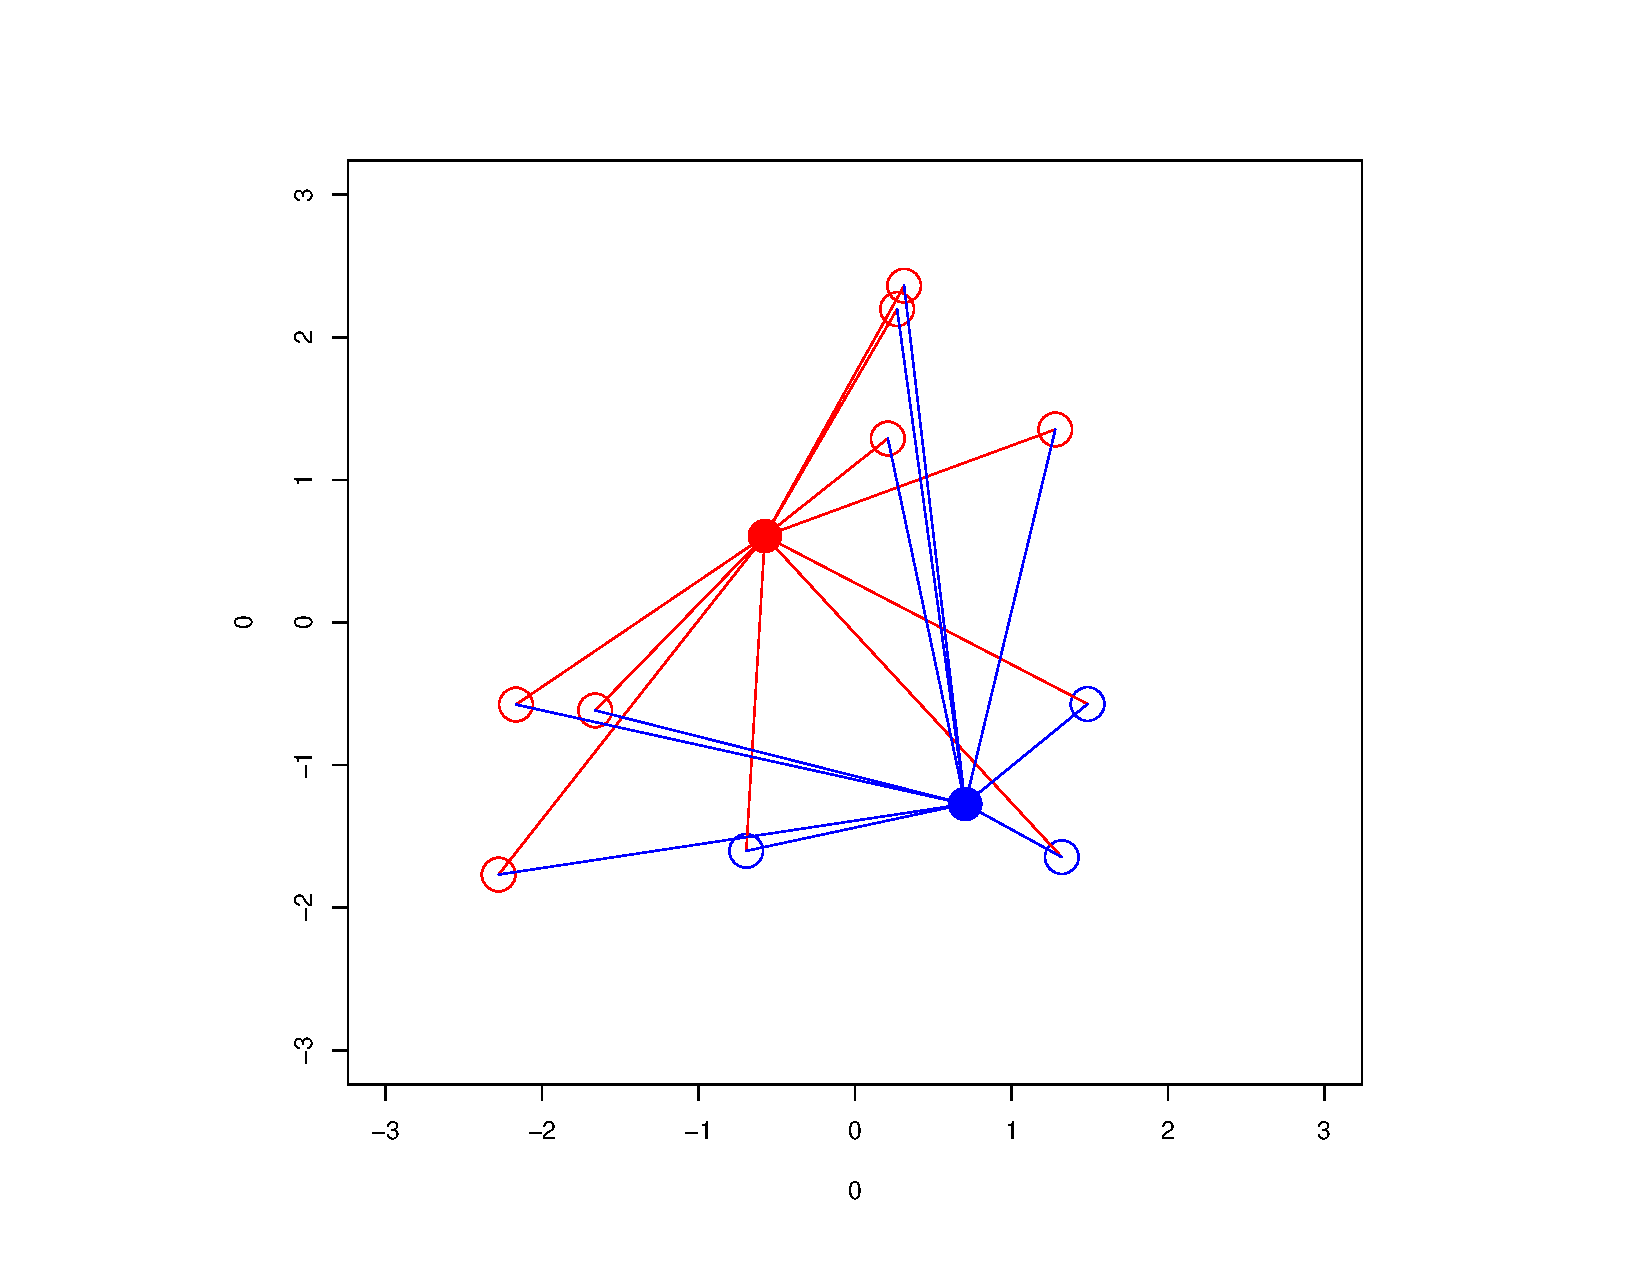
\includegraphics[width=0.7\textwidth ]{fig//kmeans206}
 }
 \frame{\frametitle{}
 \centering
 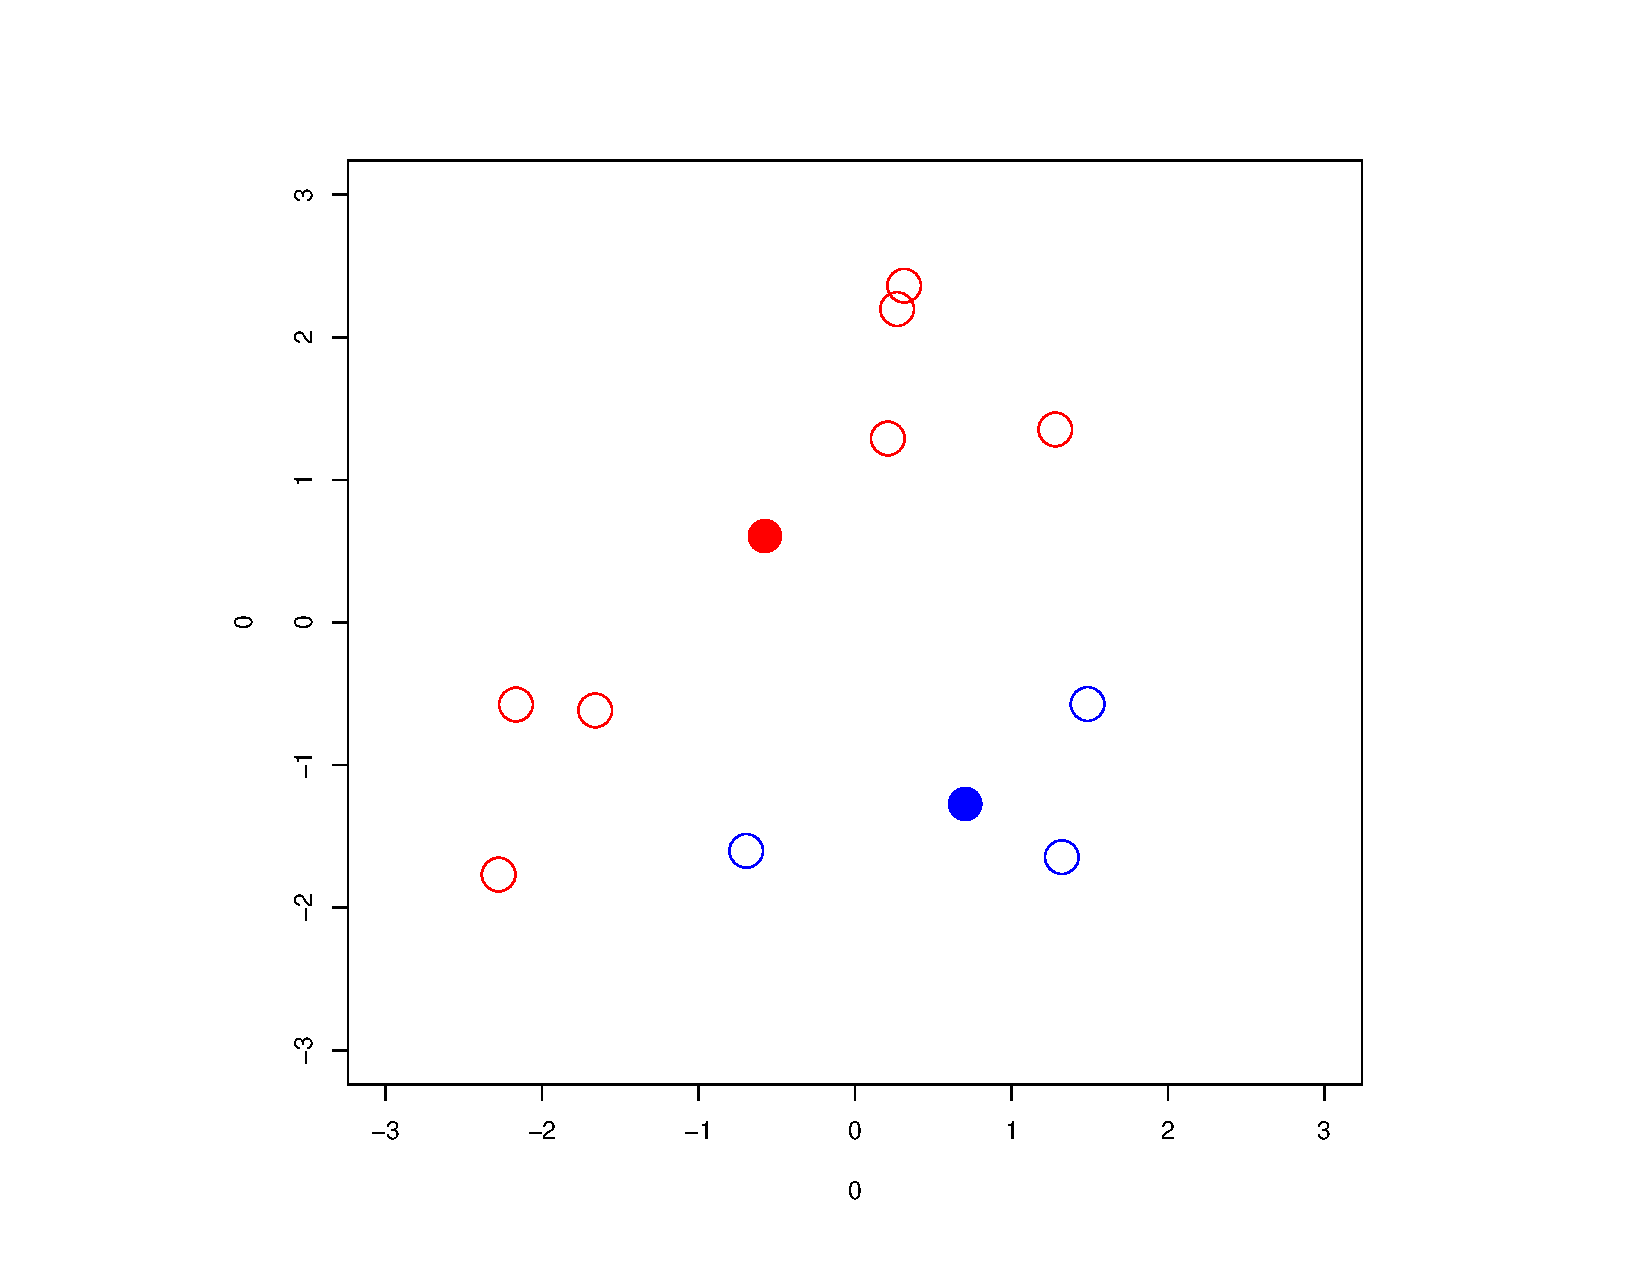
\includegraphics[width=0.7\textwidth ]{fig//kmeans205}
 }


 
 \frame{\frametitle{Compare 1}
 \centering
 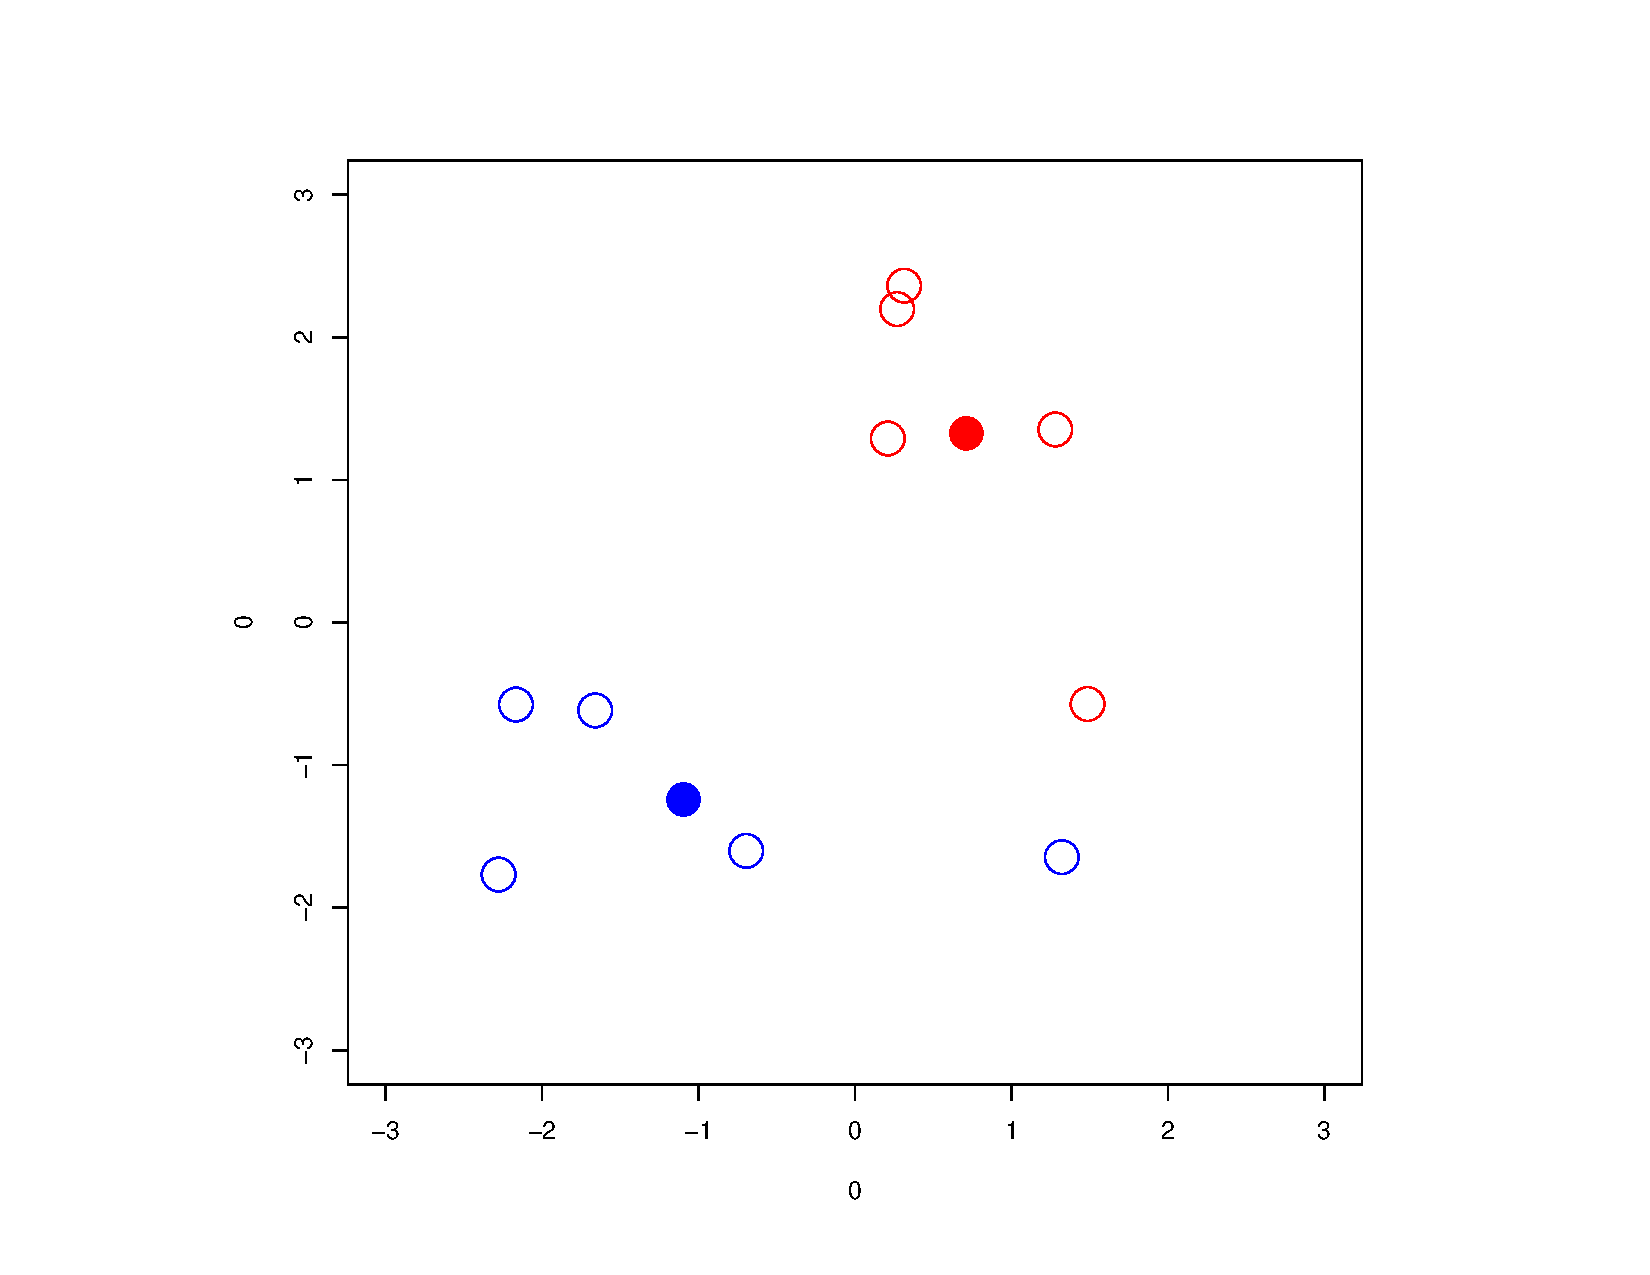
\includegraphics[width=0.7\textwidth ]{fig//kmeans105}
 }
 \frame{\frametitle{Compare 2}
 \centering
 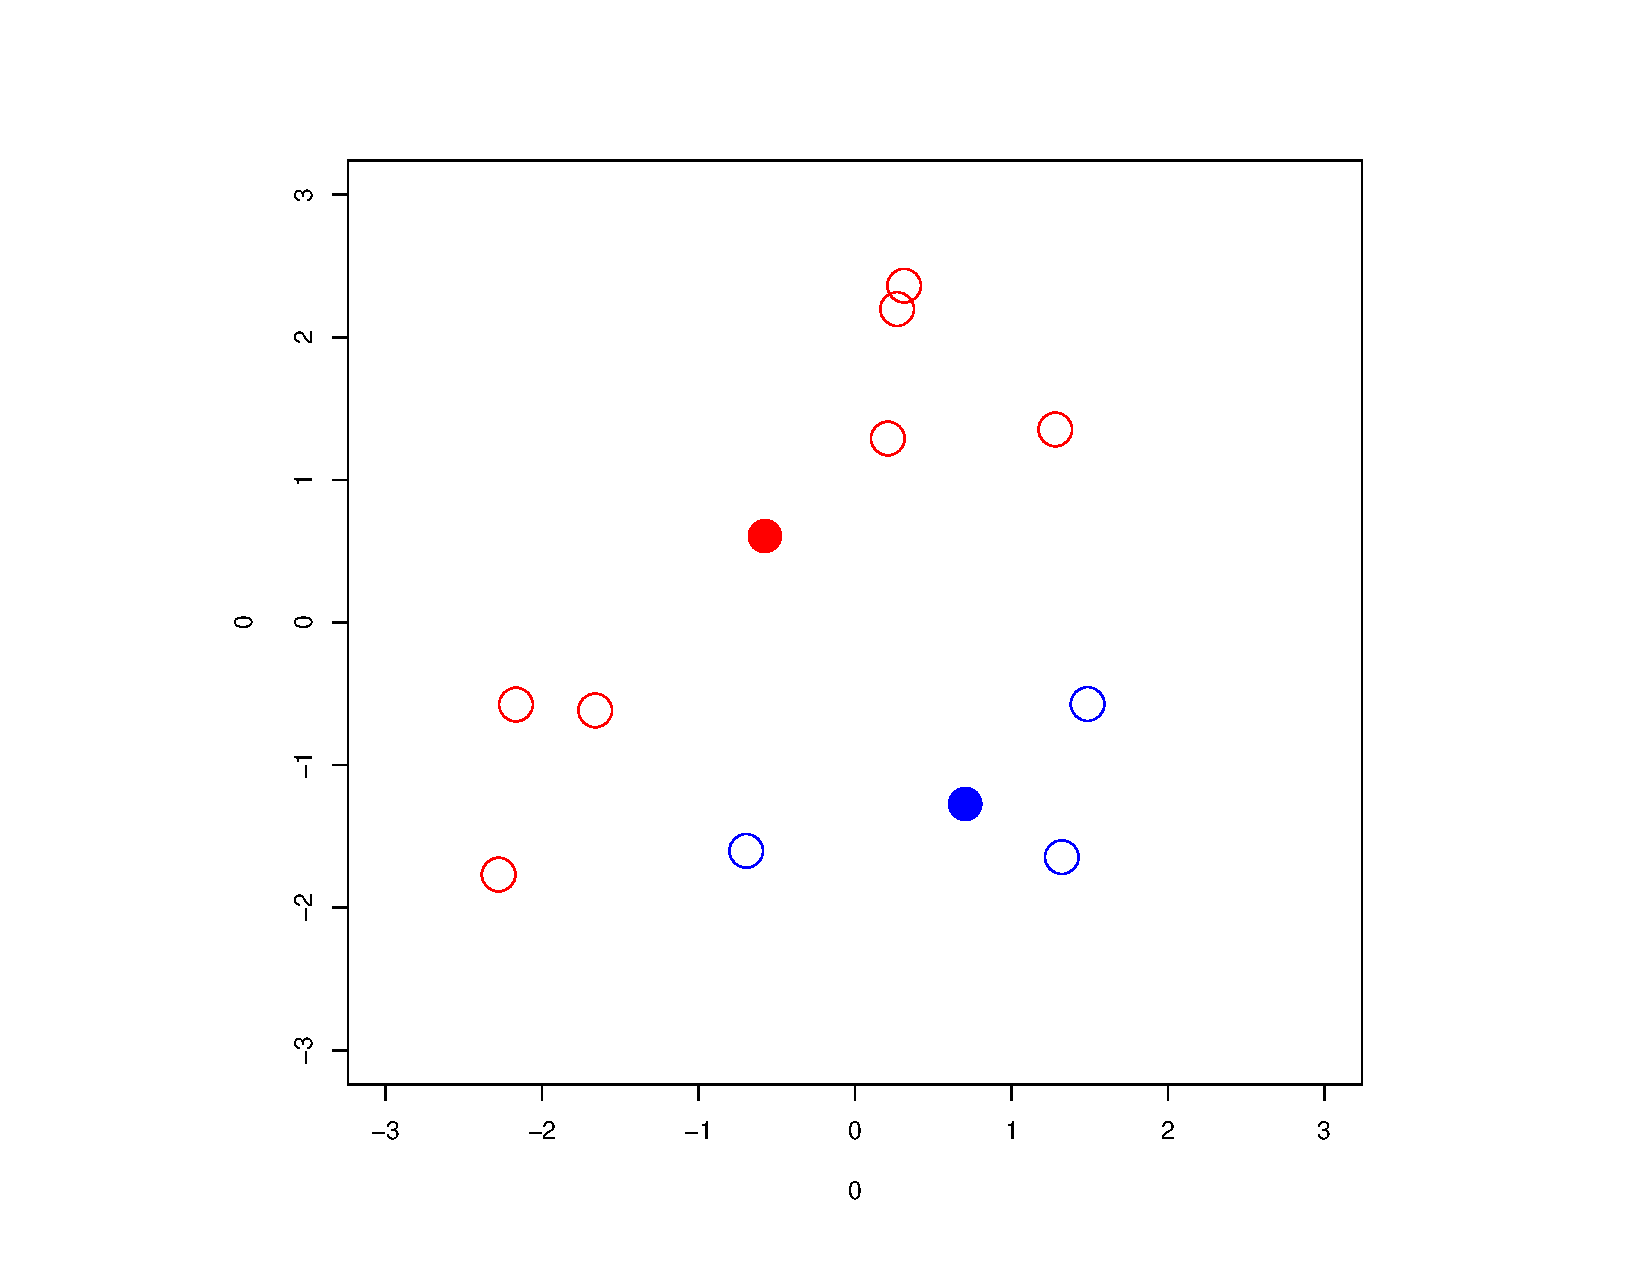
\includegraphics[width=0.7\textwidth ]{fig//kmeans205}
 }
 


\frame{\frametitle{Formalism}
 \begin{equation}
S_T=S_W(\dvec)+S_B(\dvec),
%\label{eq:cluster:intro:general:anvar}
\end{equation}
in which 
\begin{eqnarray}
S_W(\dvec)&=&\sum_{c=1}^k
\sum_{\{i\mid d_i=c\}}\sum_{\{i'\mid d_{i'}=c\}} (y_{ci}-\ybar_c)^2,\\
S_B(\dvec)&=&\sum_{c=1}^k\sum_{\{i\mid d_i=c\}}\sum_{\{i'\mid d_{i'}\neq
  c\}} (y_{ci}-\ybar_c)^2
\end{eqnarray}
}
 



\section{Hierarchical Clustering}


  \frame{\frametitle{Grouping Data}
 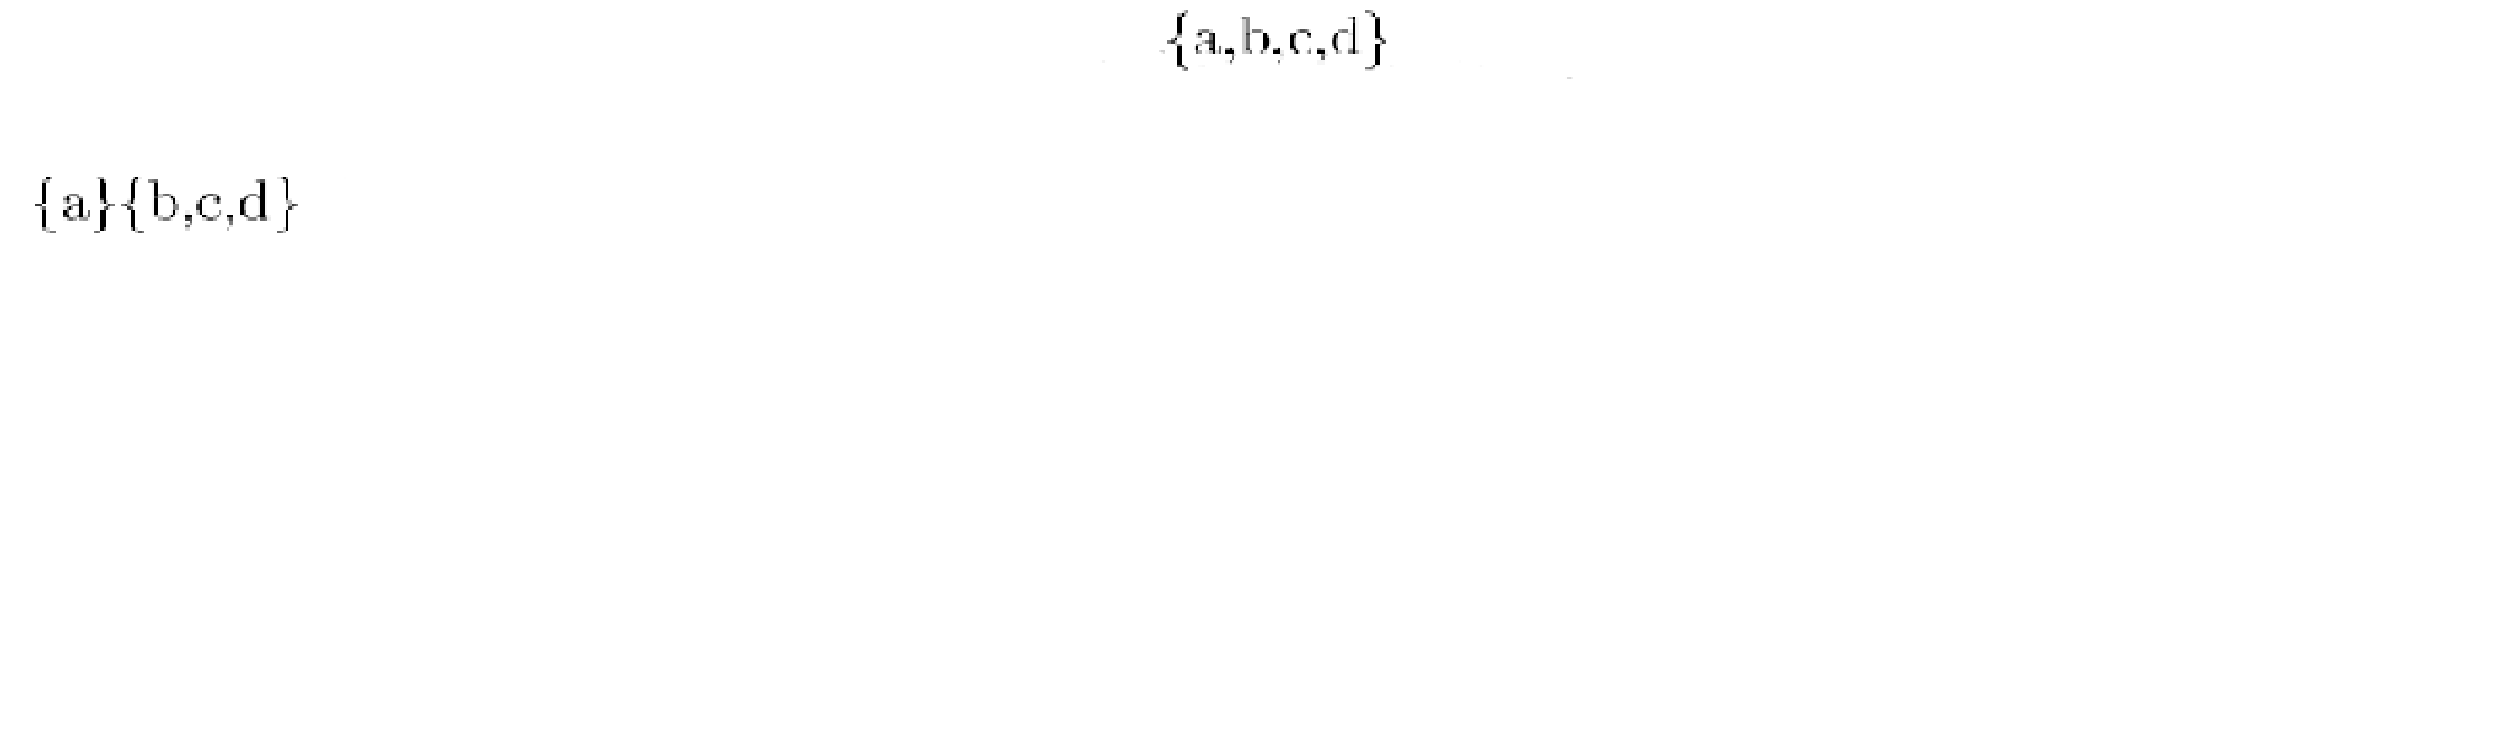
\includegraphics[width=\textwidth]{fig/part2-1}\\
 \begin{center}
 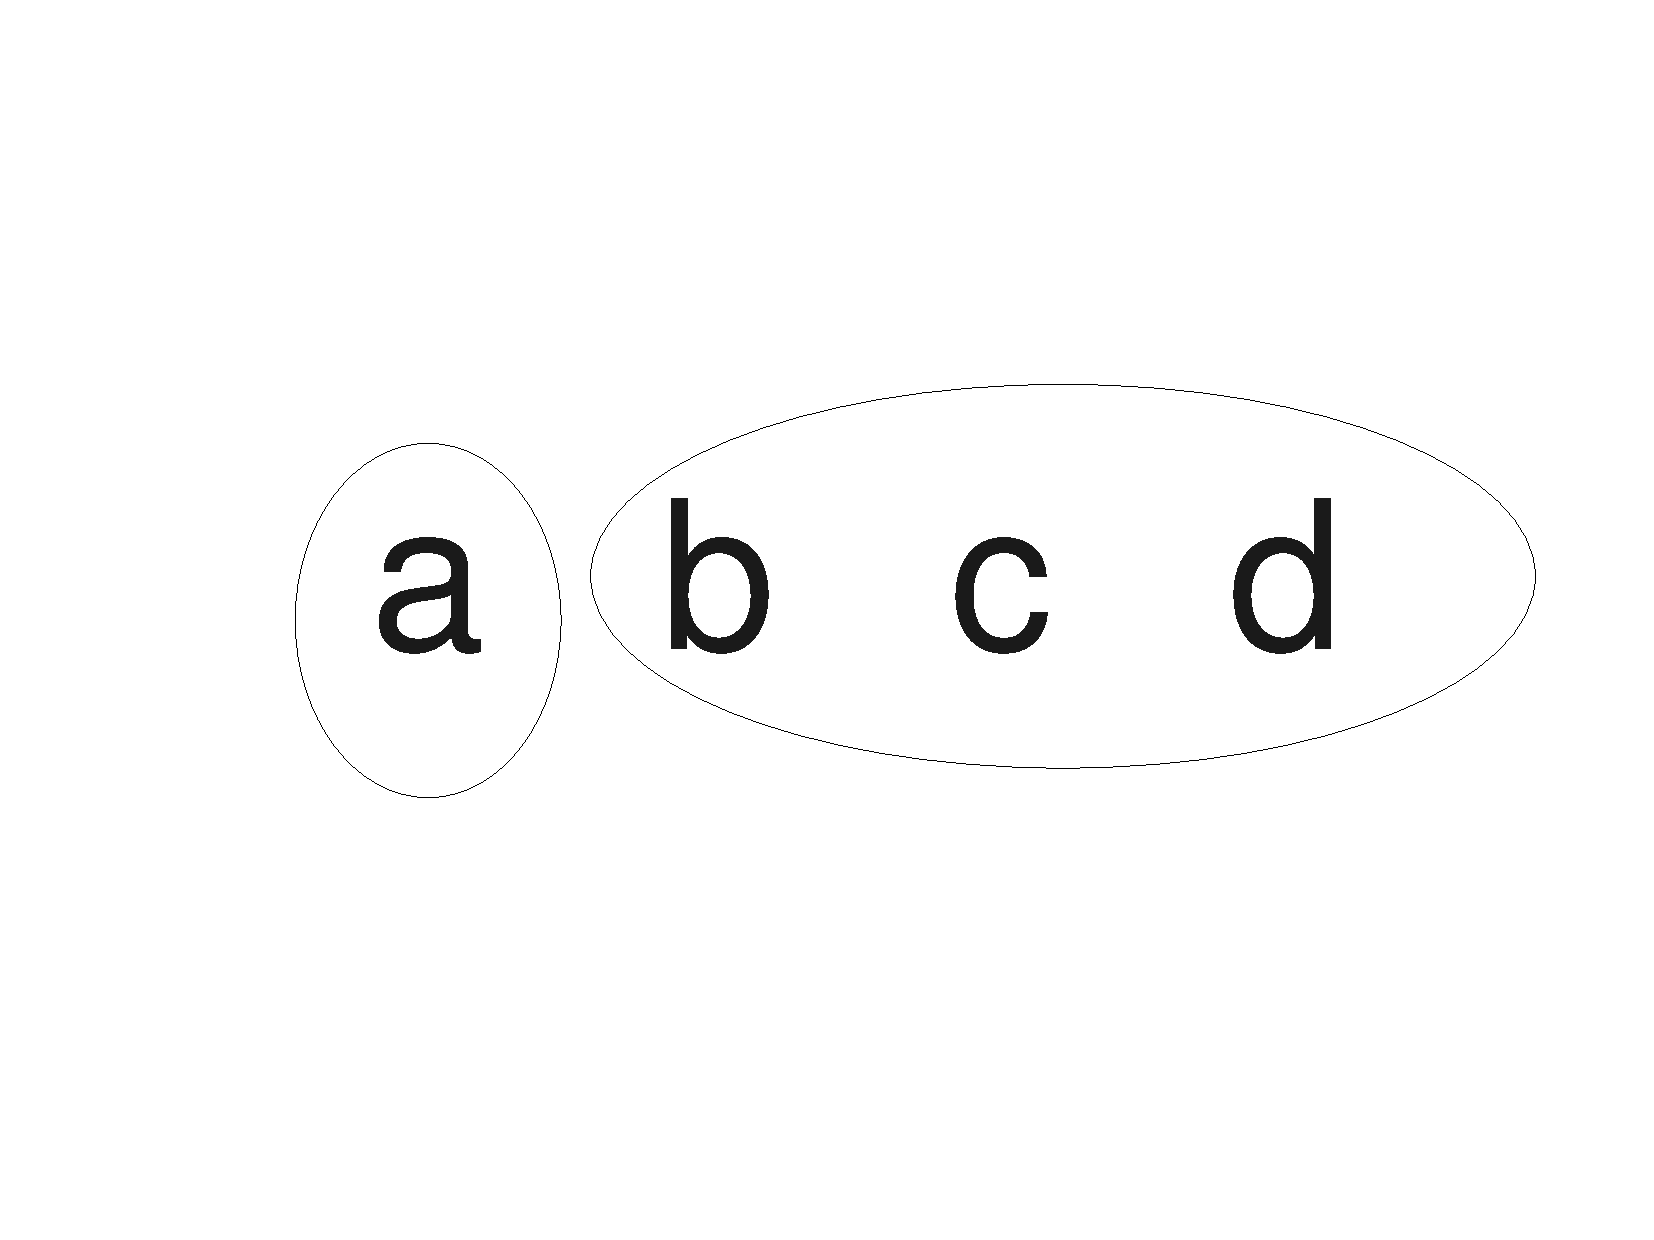
\includegraphics[width=0.5\textwidth]{fig/abcd2-1}
 \end{center}
 }
 
 
  \frame{\frametitle{}
 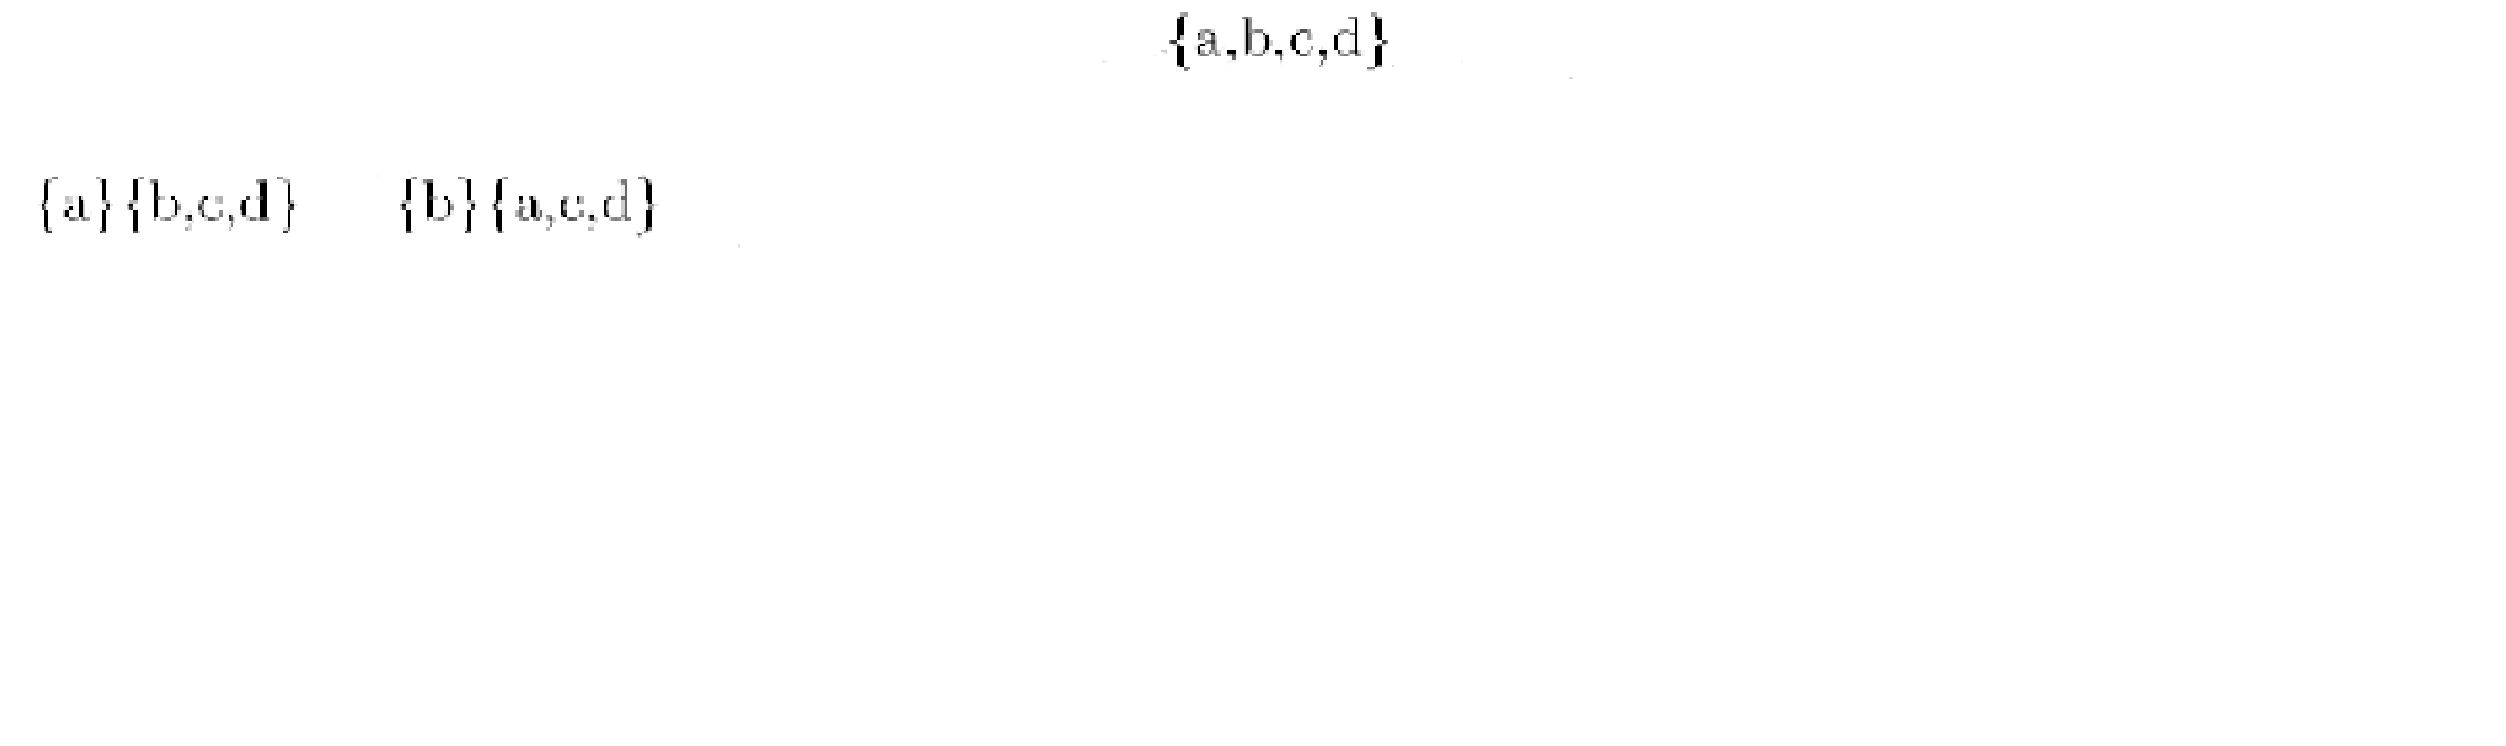
\includegraphics[width=\textwidth]{fig/part2-2}\\
 \begin{center}
 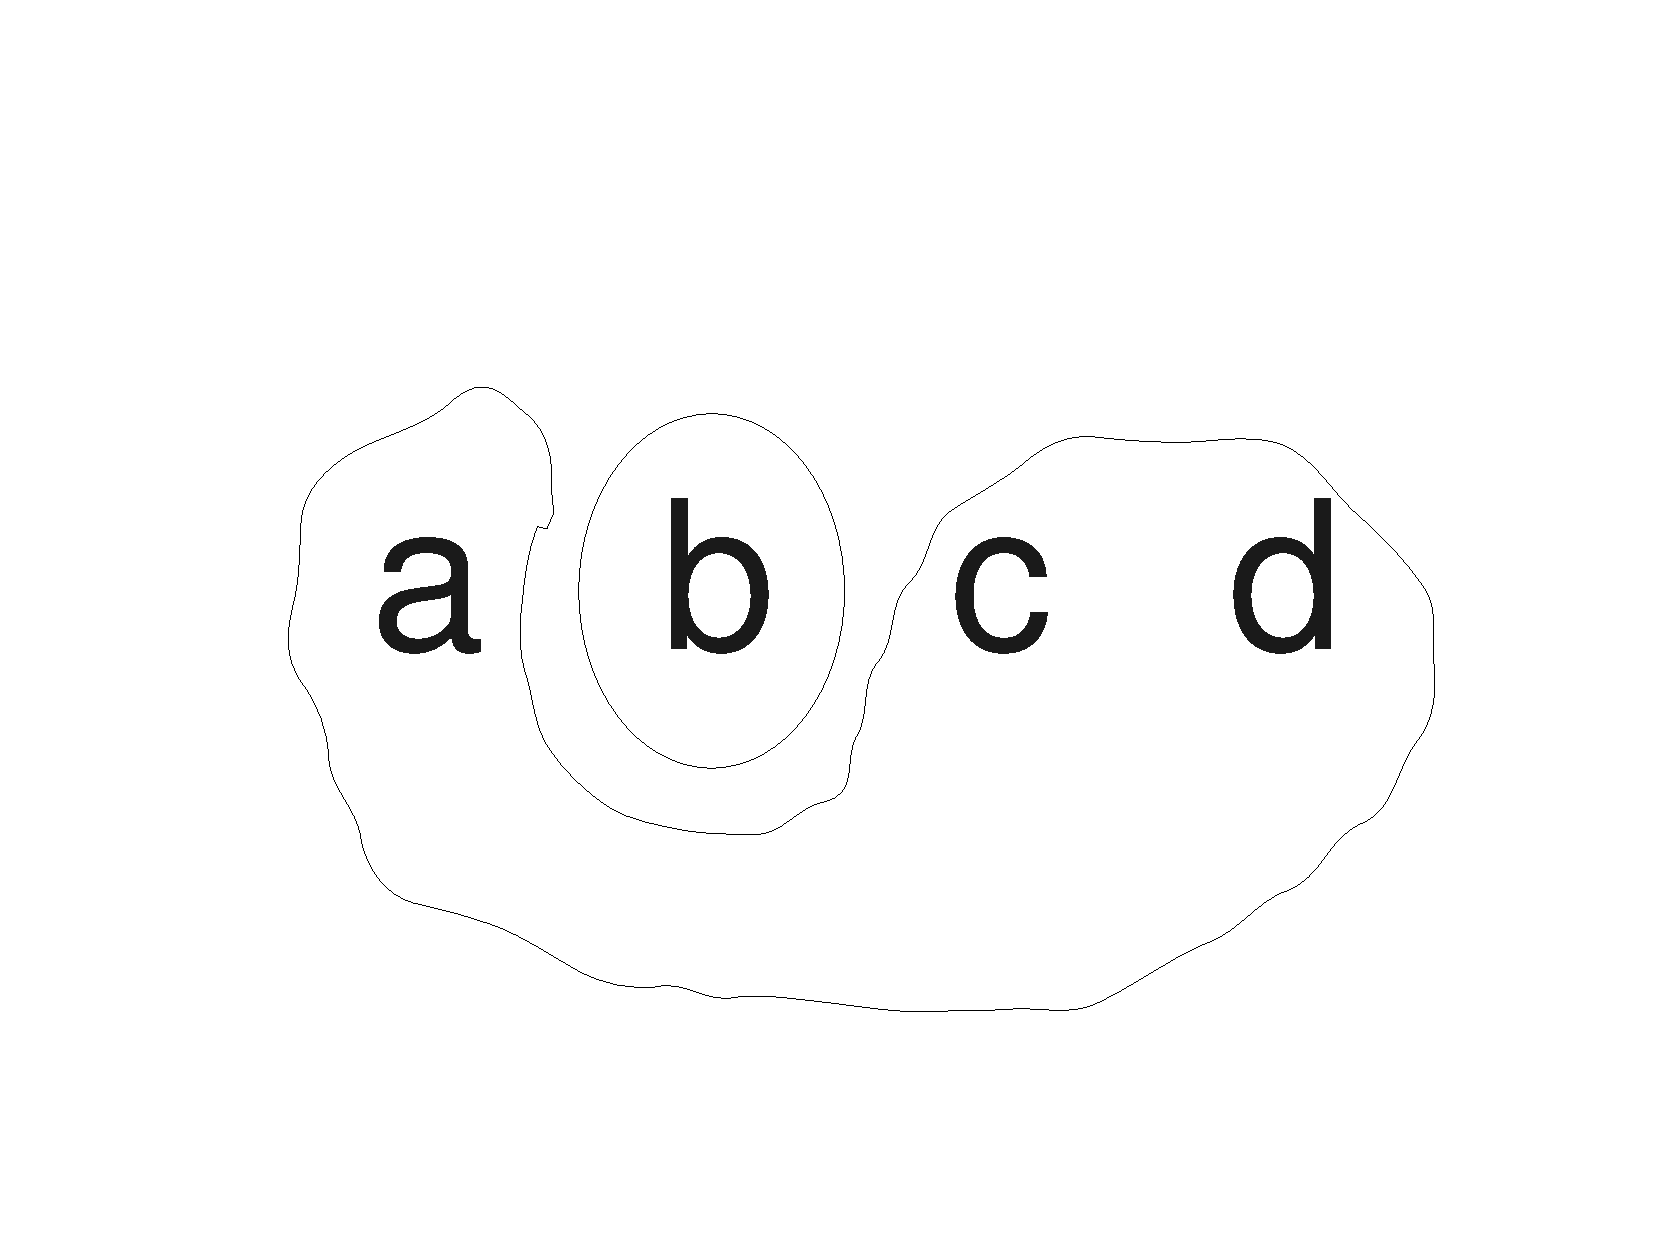
\includegraphics[width=0.5\textwidth]{fig/abcd2-2}
 \end{center}
 }
 
  \frame{\frametitle{}
 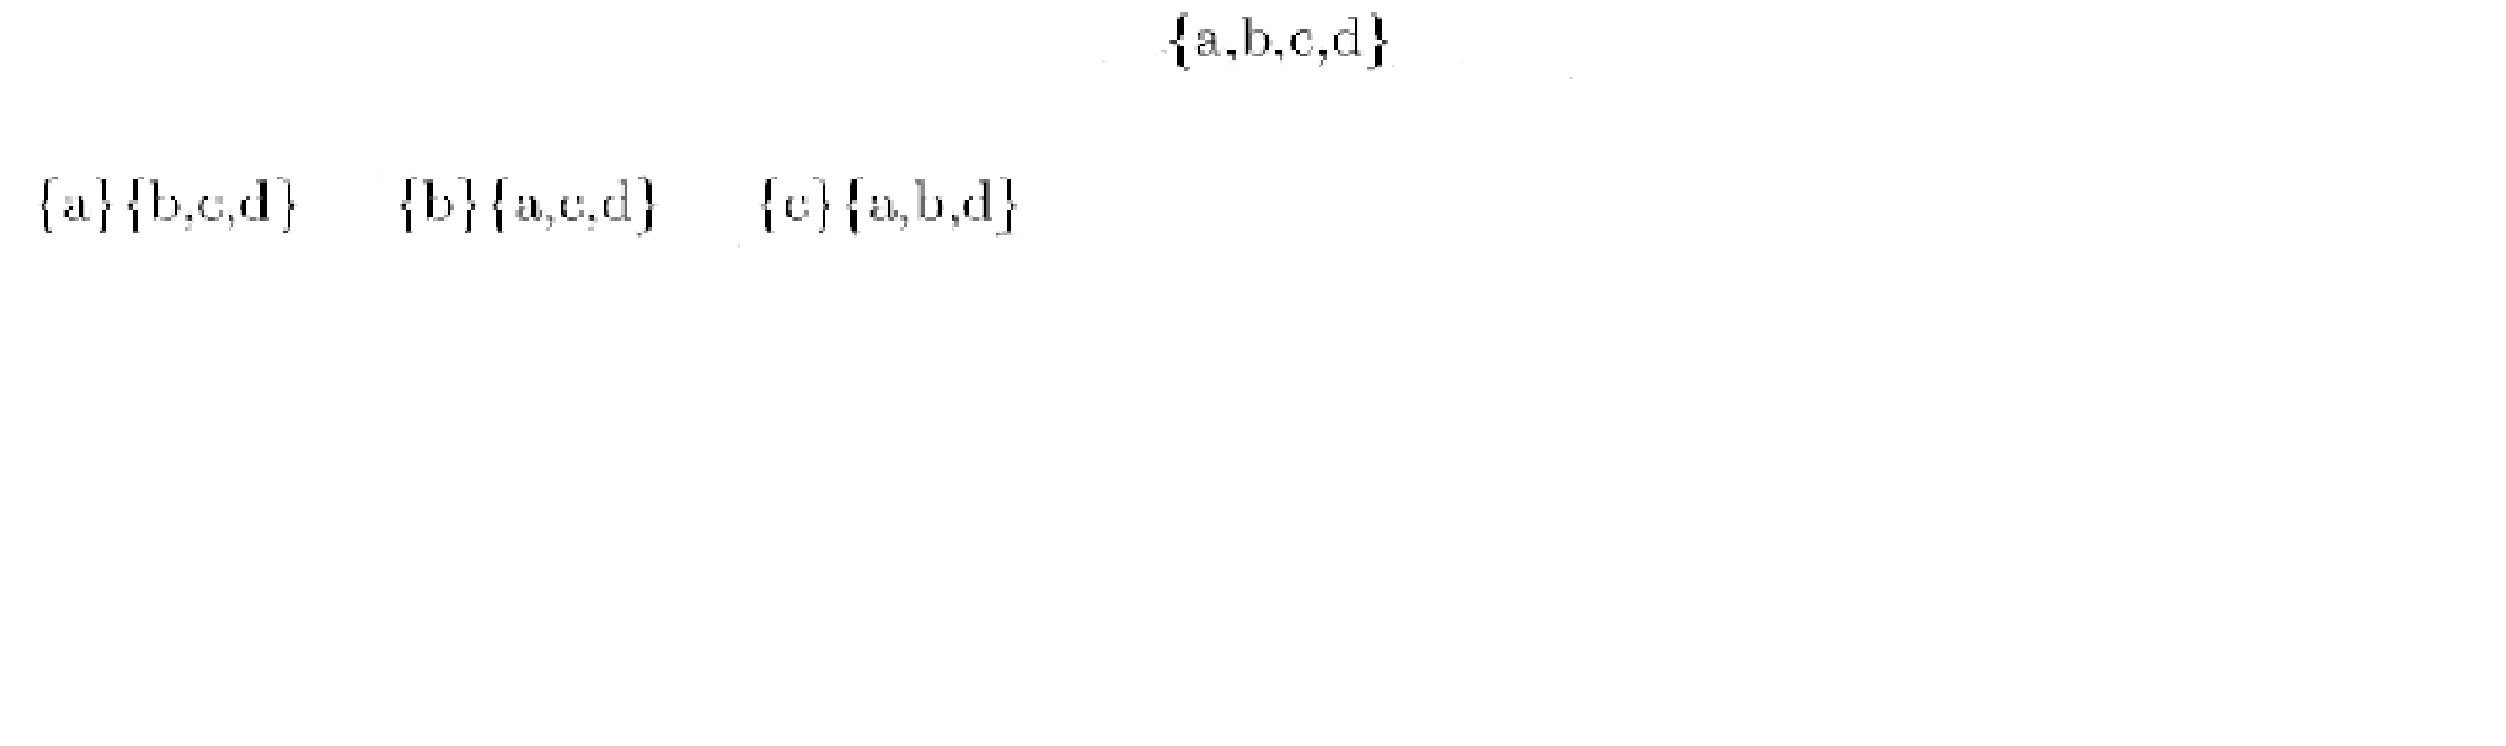
\includegraphics[width=\textwidth]{fig/part2-3}\\
 \begin{center}
 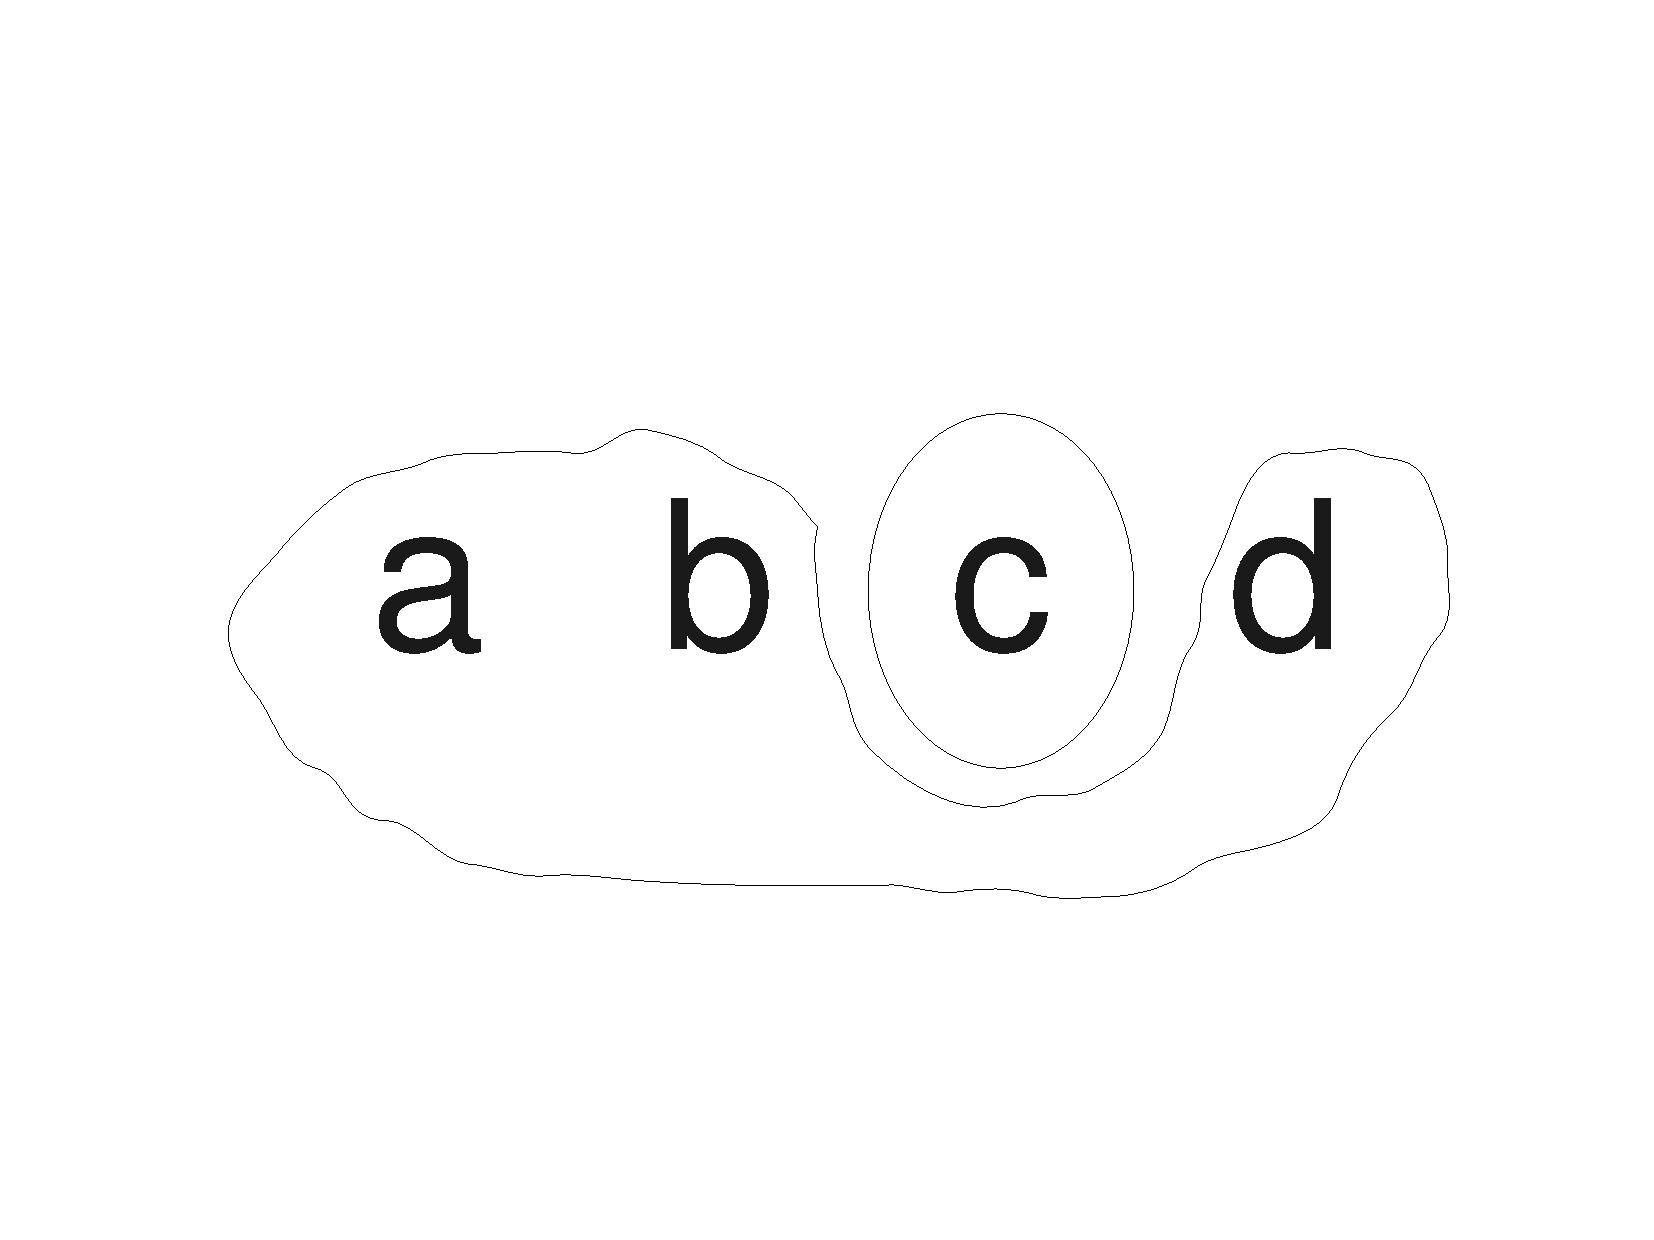
\includegraphics[width=0.5\textwidth]{fig/abcd2-3}
 \end{center}
 }
 
  \frame{\frametitle{}
 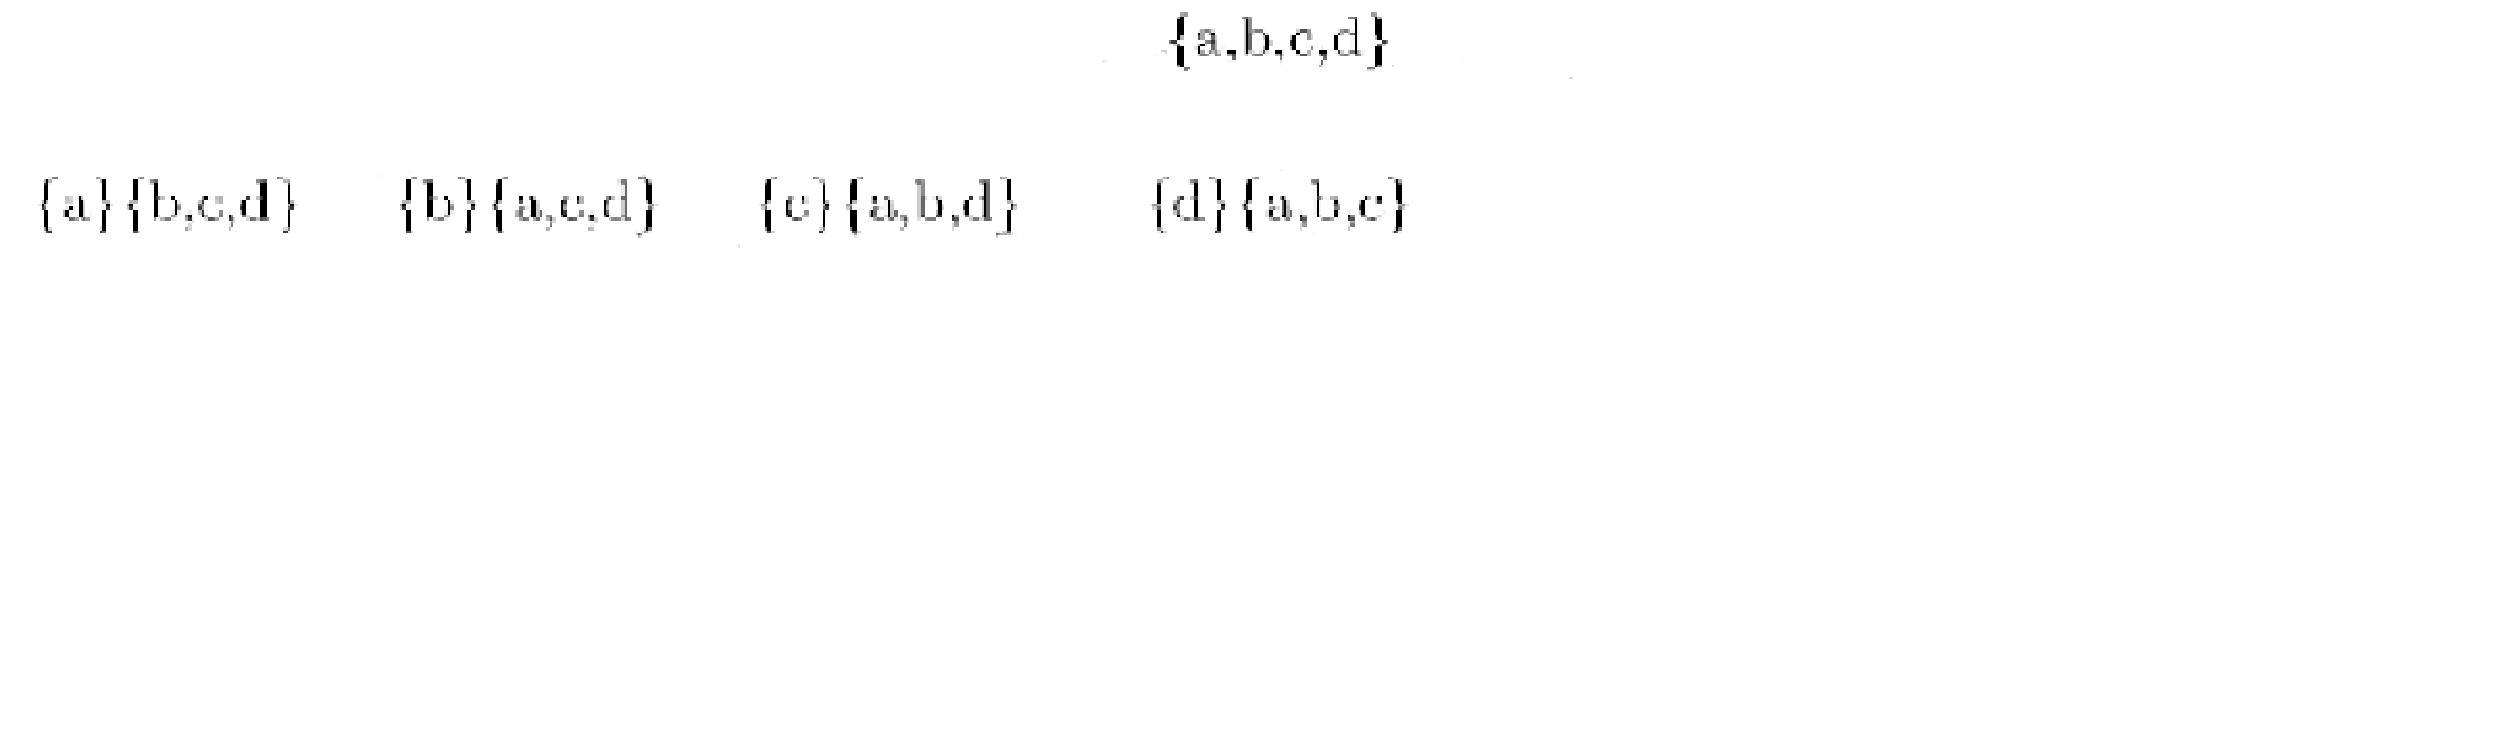
\includegraphics[width=\textwidth]{fig/part2-4}\\
 \begin{center}
 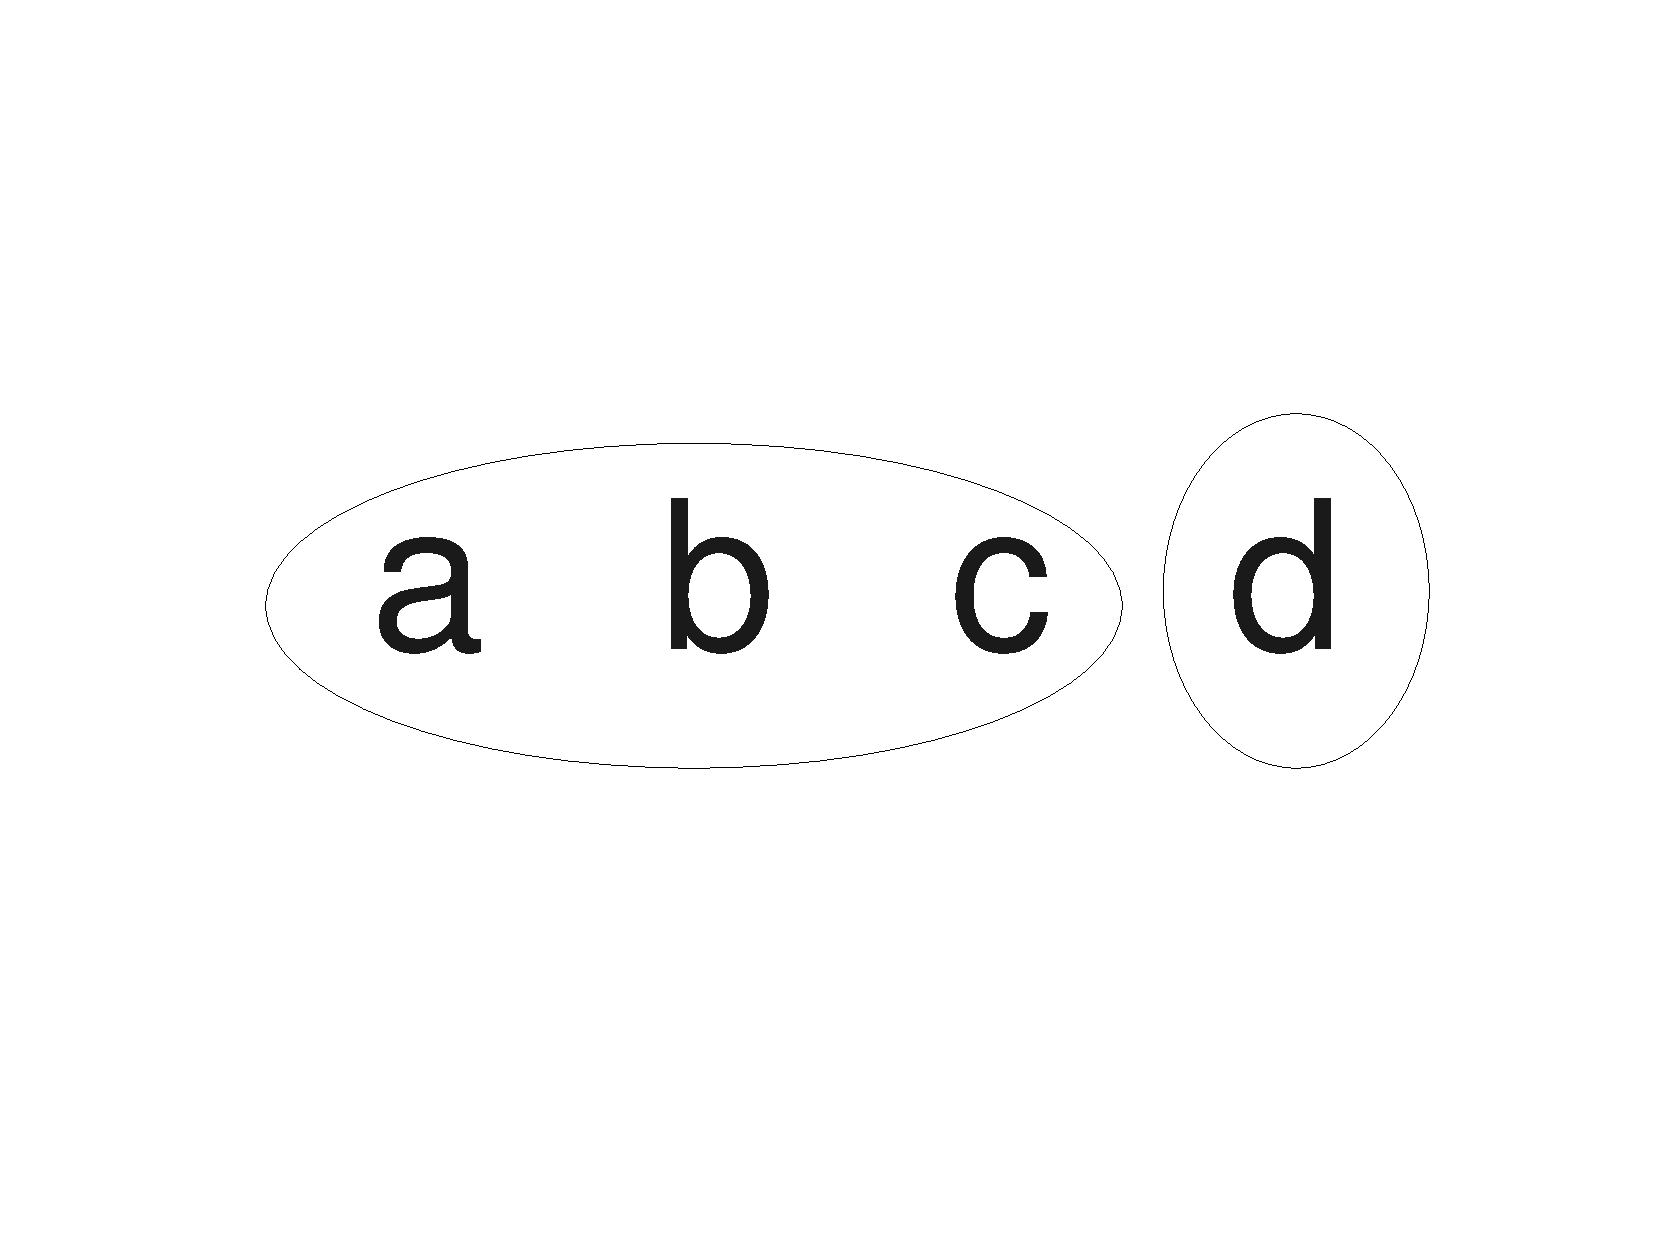
\includegraphics[width=0.5\textwidth]{fig/abcd2-4}
 \end{center}
 }
 
  \frame{\frametitle{}
 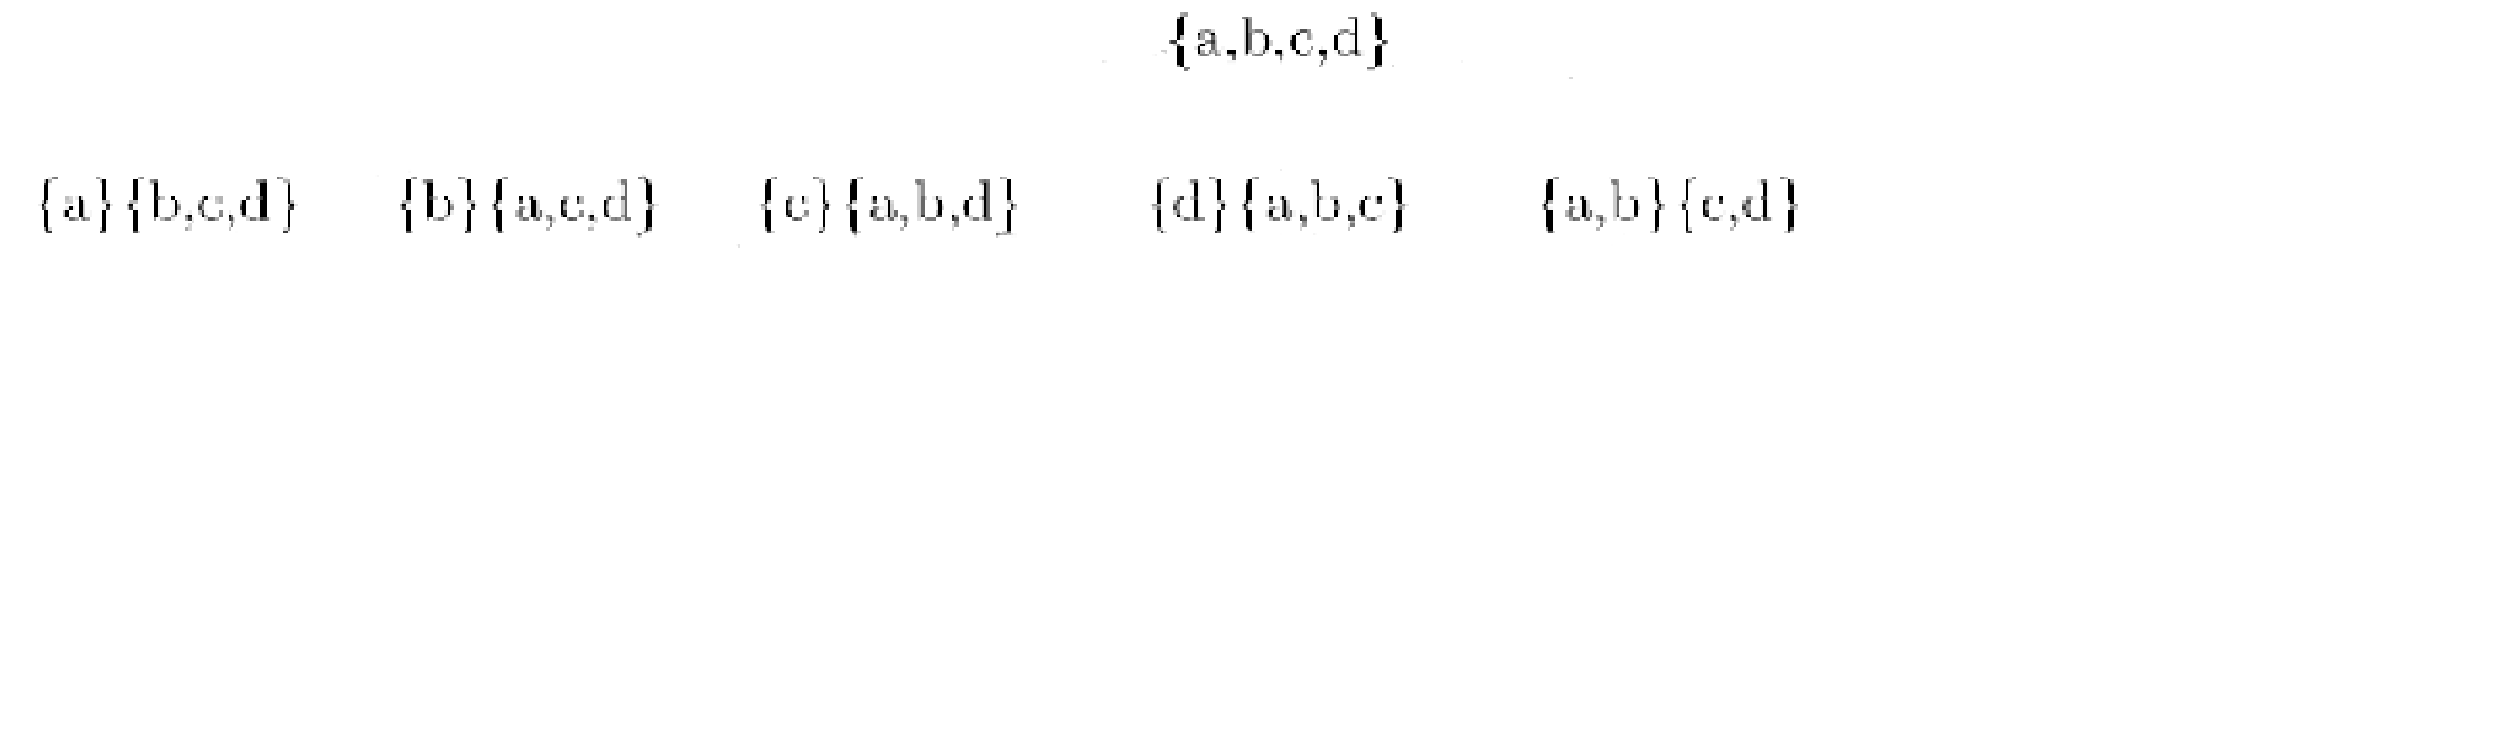
\includegraphics[width=\textwidth]{fig/part2-5}\\
 \begin{center}
 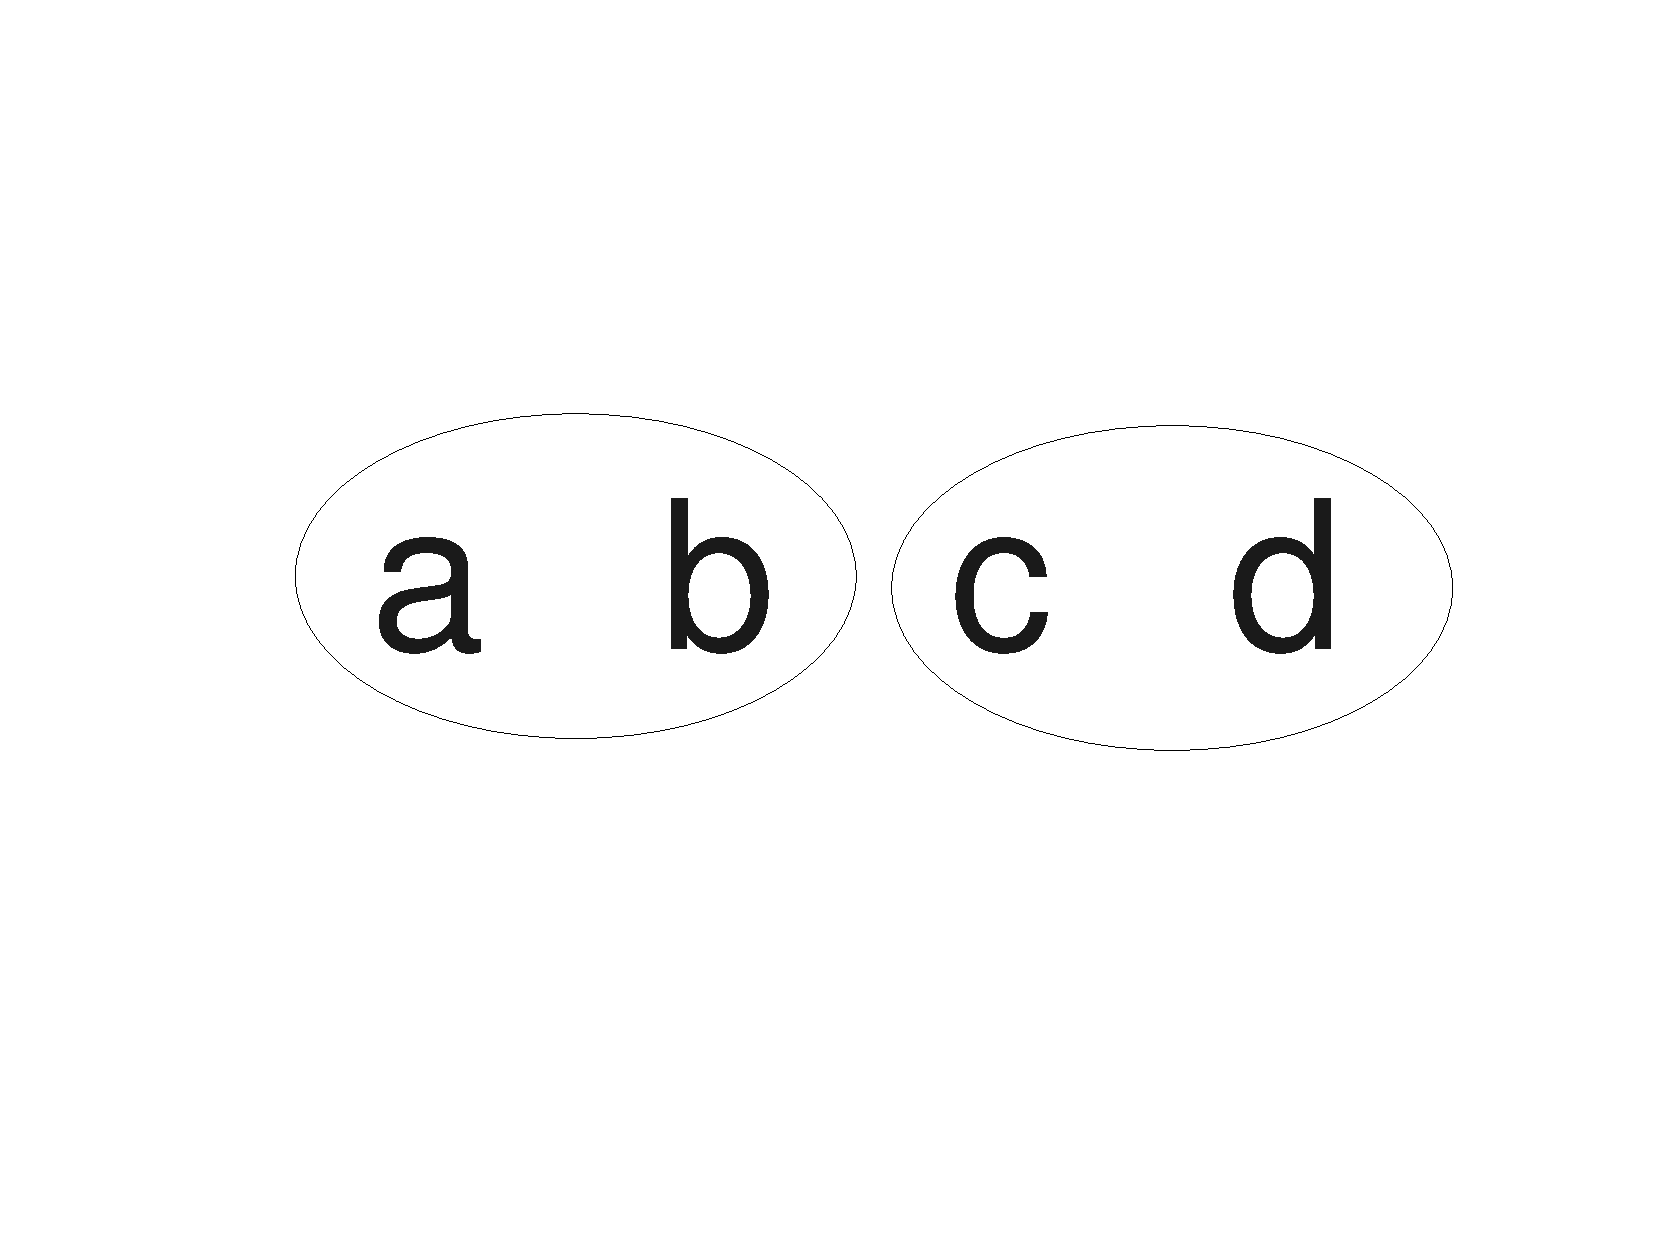
\includegraphics[width=0.5\textwidth]{fig/abcd2-5}
 \end{center}
 }
 
  \frame{\frametitle{}
 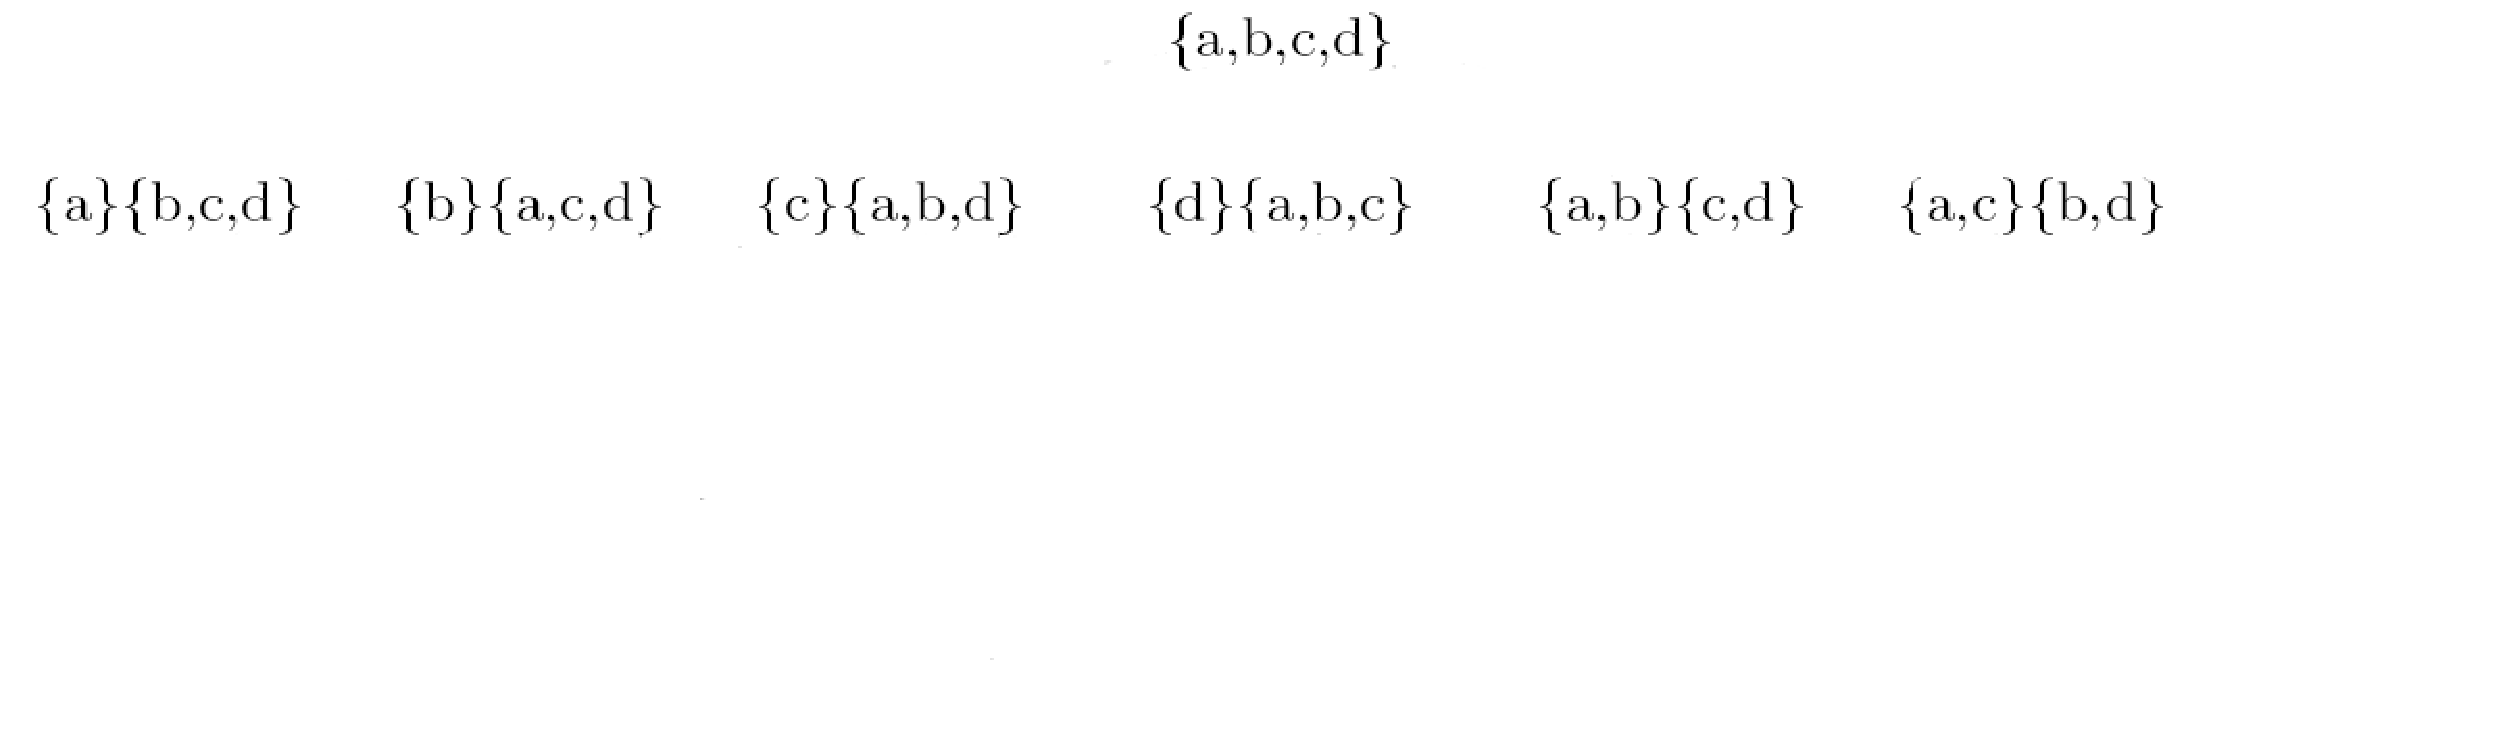
\includegraphics[width=\textwidth]{fig/part2-6}\\
 \begin{center}
 
\includegraphics[width=0.5\textwidth]{fig/abcd2-6}
 \end{center}
 }
 
  \frame{\frametitle{}
 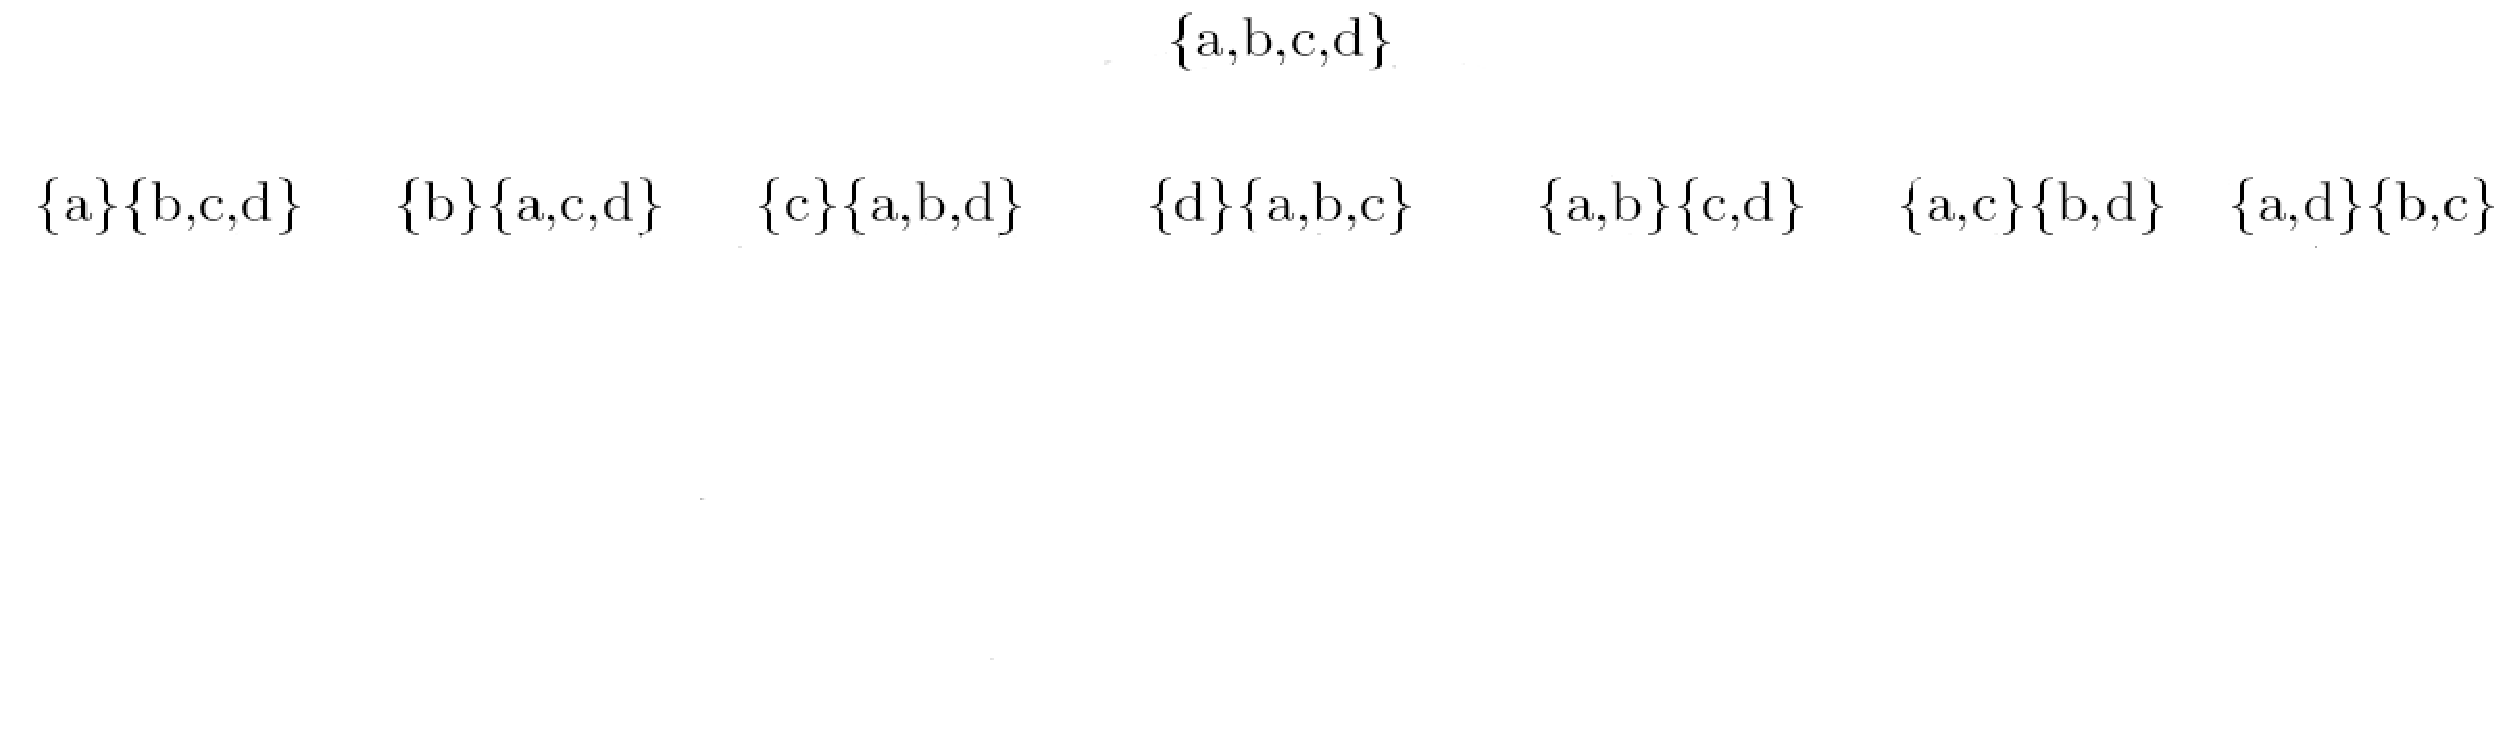
\includegraphics[width=\textwidth]{fig/part2-7}\\
 \begin{center}
 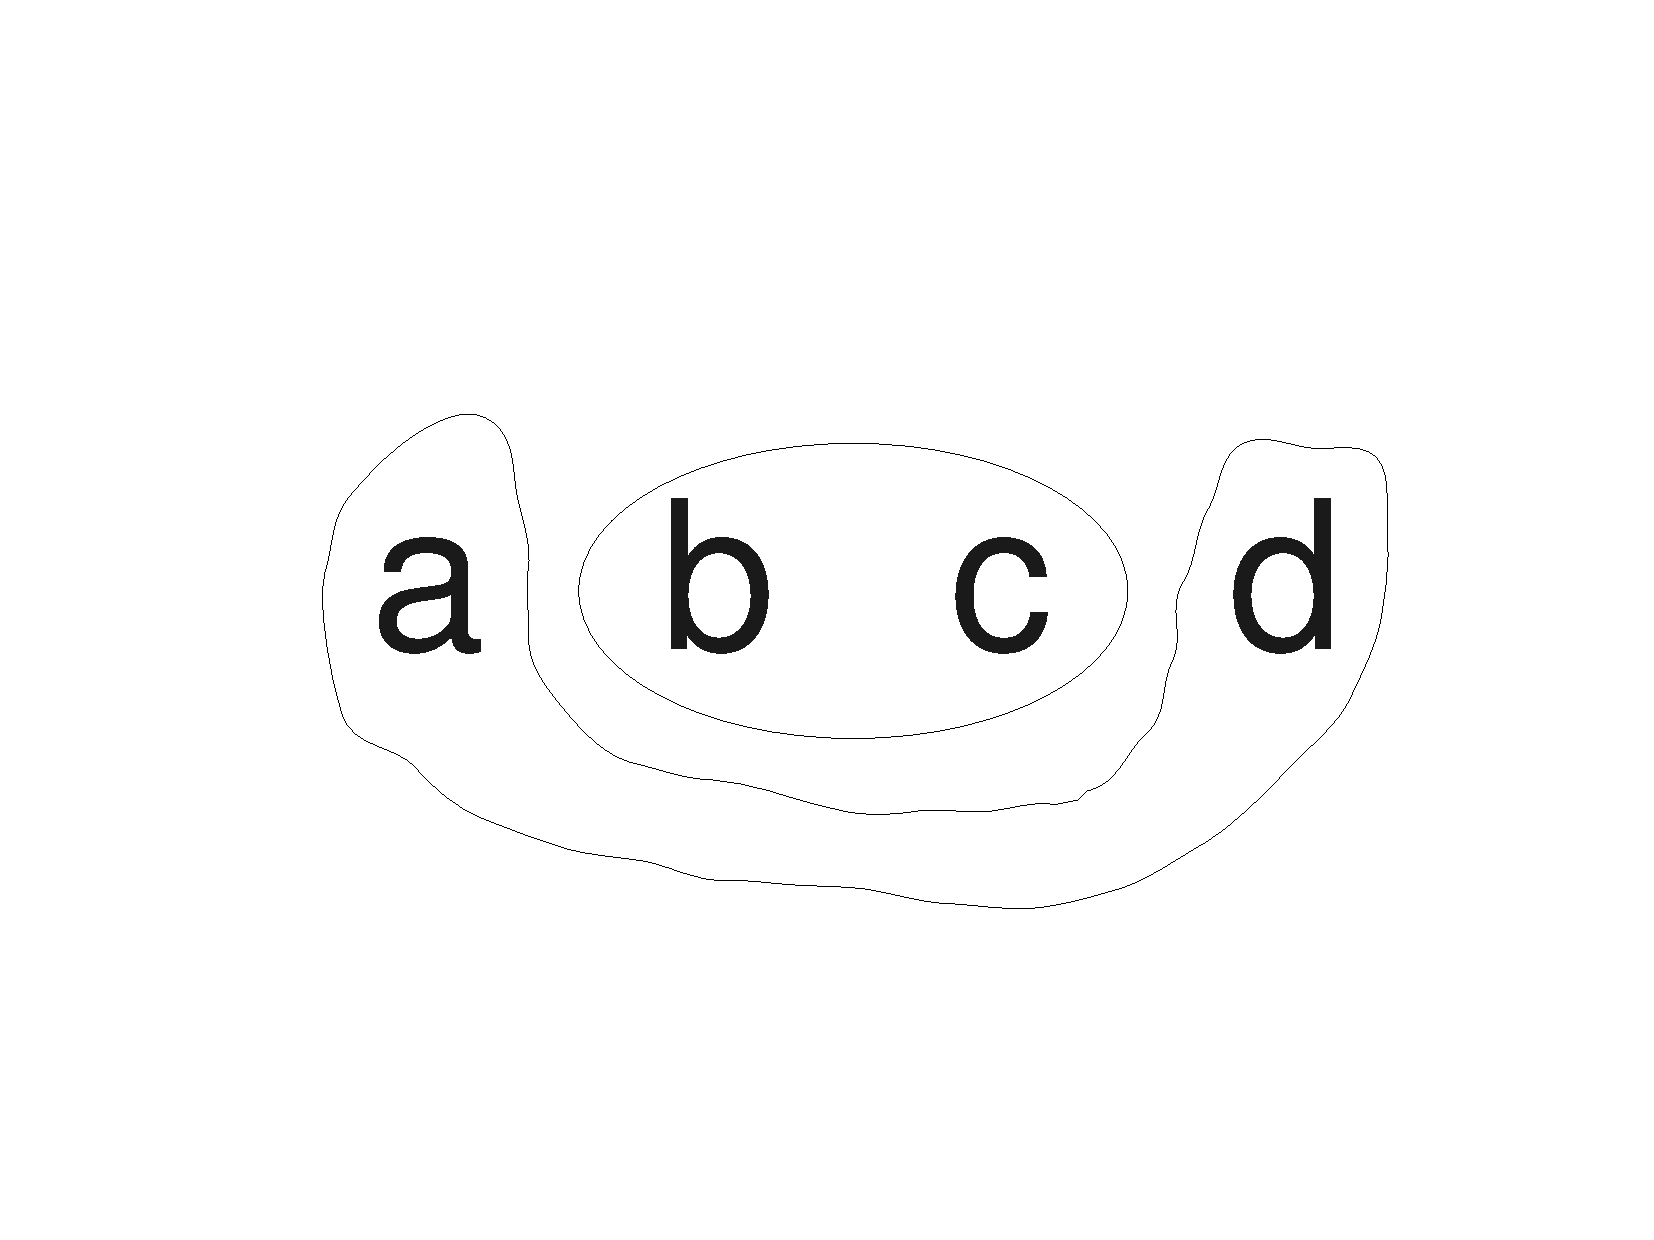
\includegraphics[width=0.5\textwidth]{fig/abcd2-7}
 \end{center}
 }
 
  \frame{\frametitle{}
 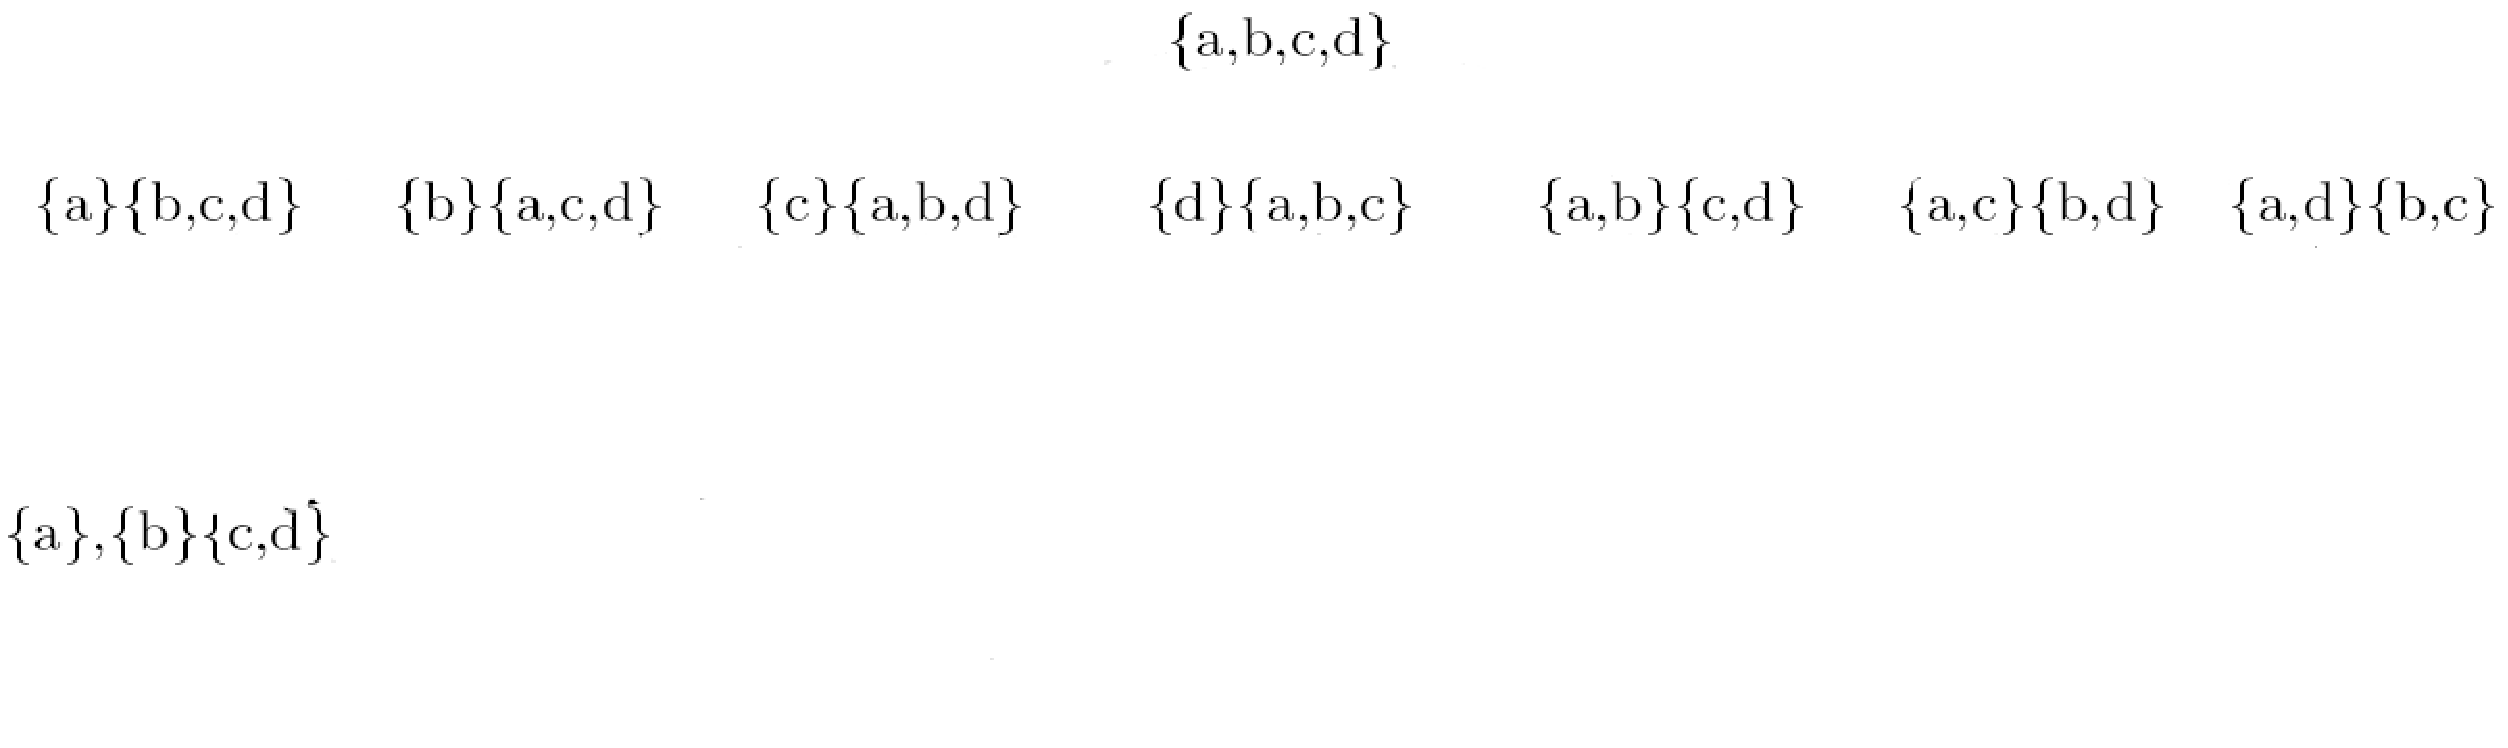
\includegraphics[width=\textwidth]{fig/part3-1}\\
 \begin{center}
 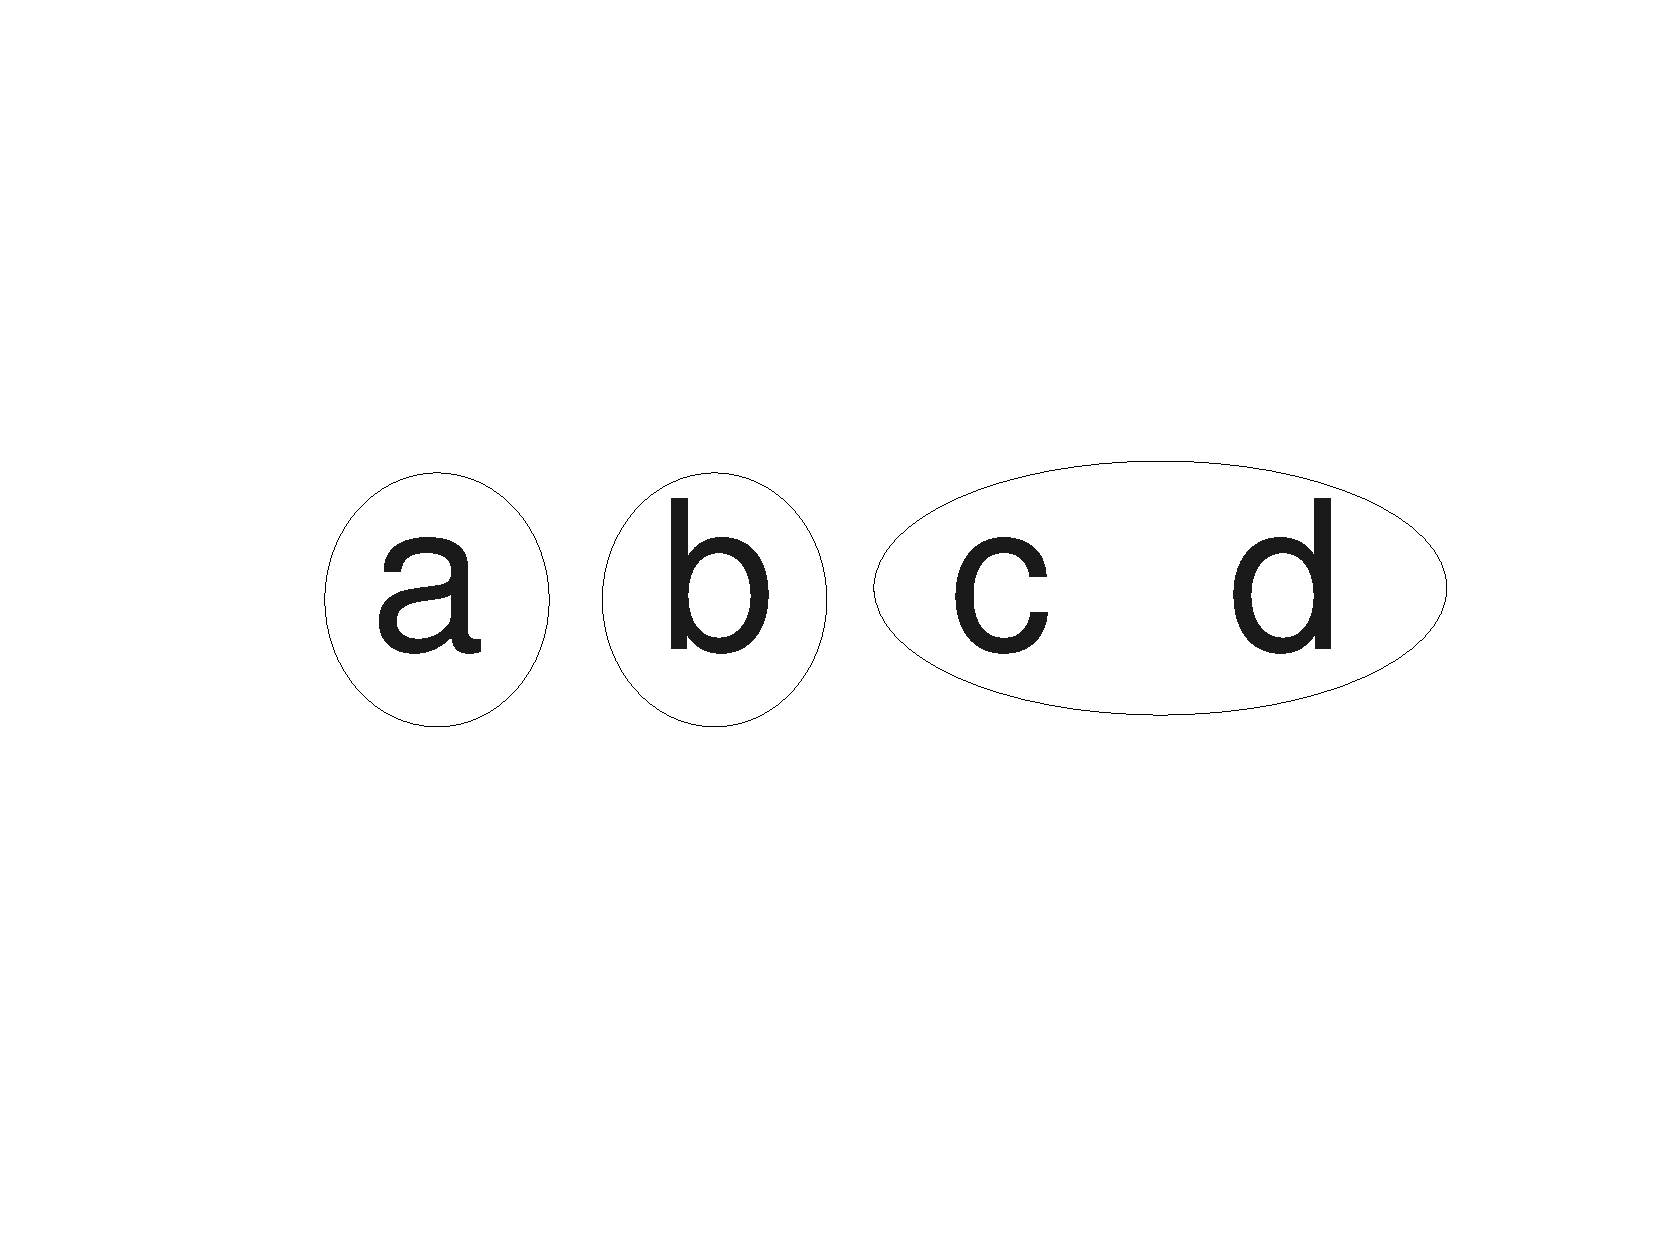
\includegraphics[width=0.5\textwidth]{fig/abcd3-1}
 \end{center}
 }
 
  \frame{\frametitle{}
 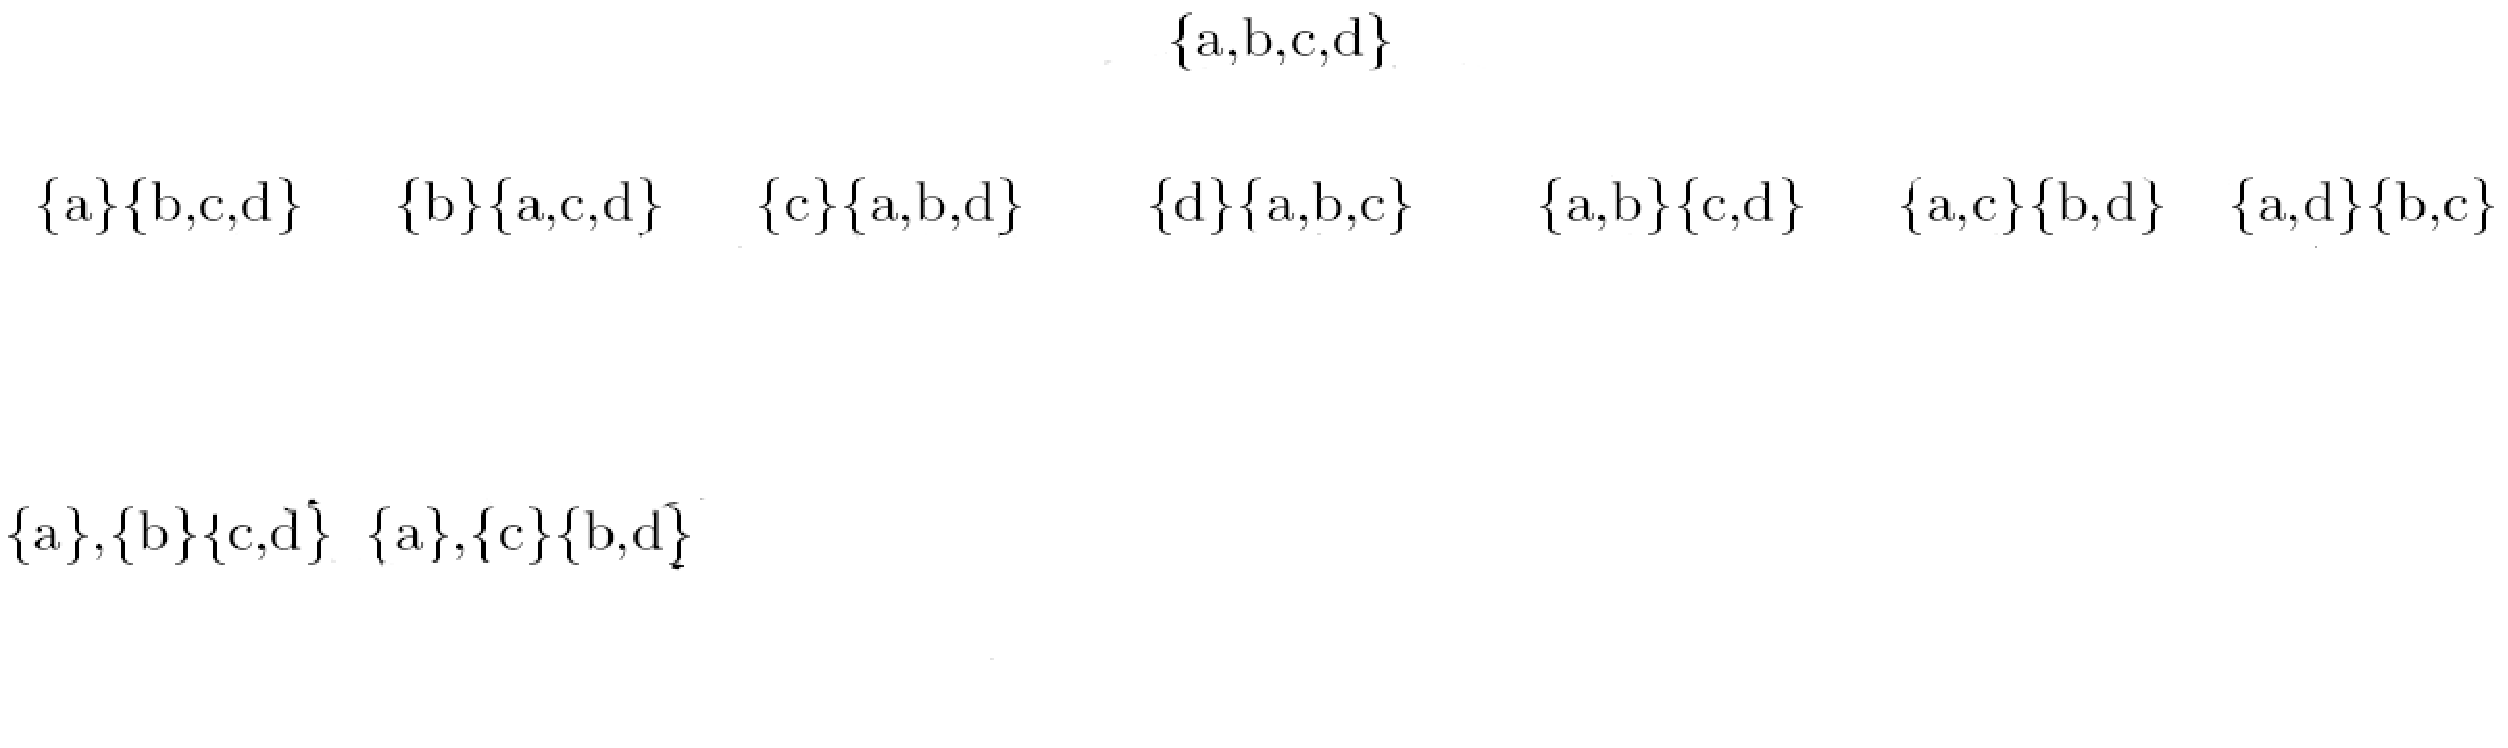
\includegraphics[width=\textwidth]{fig/part3-2}\\
 \begin{center}
 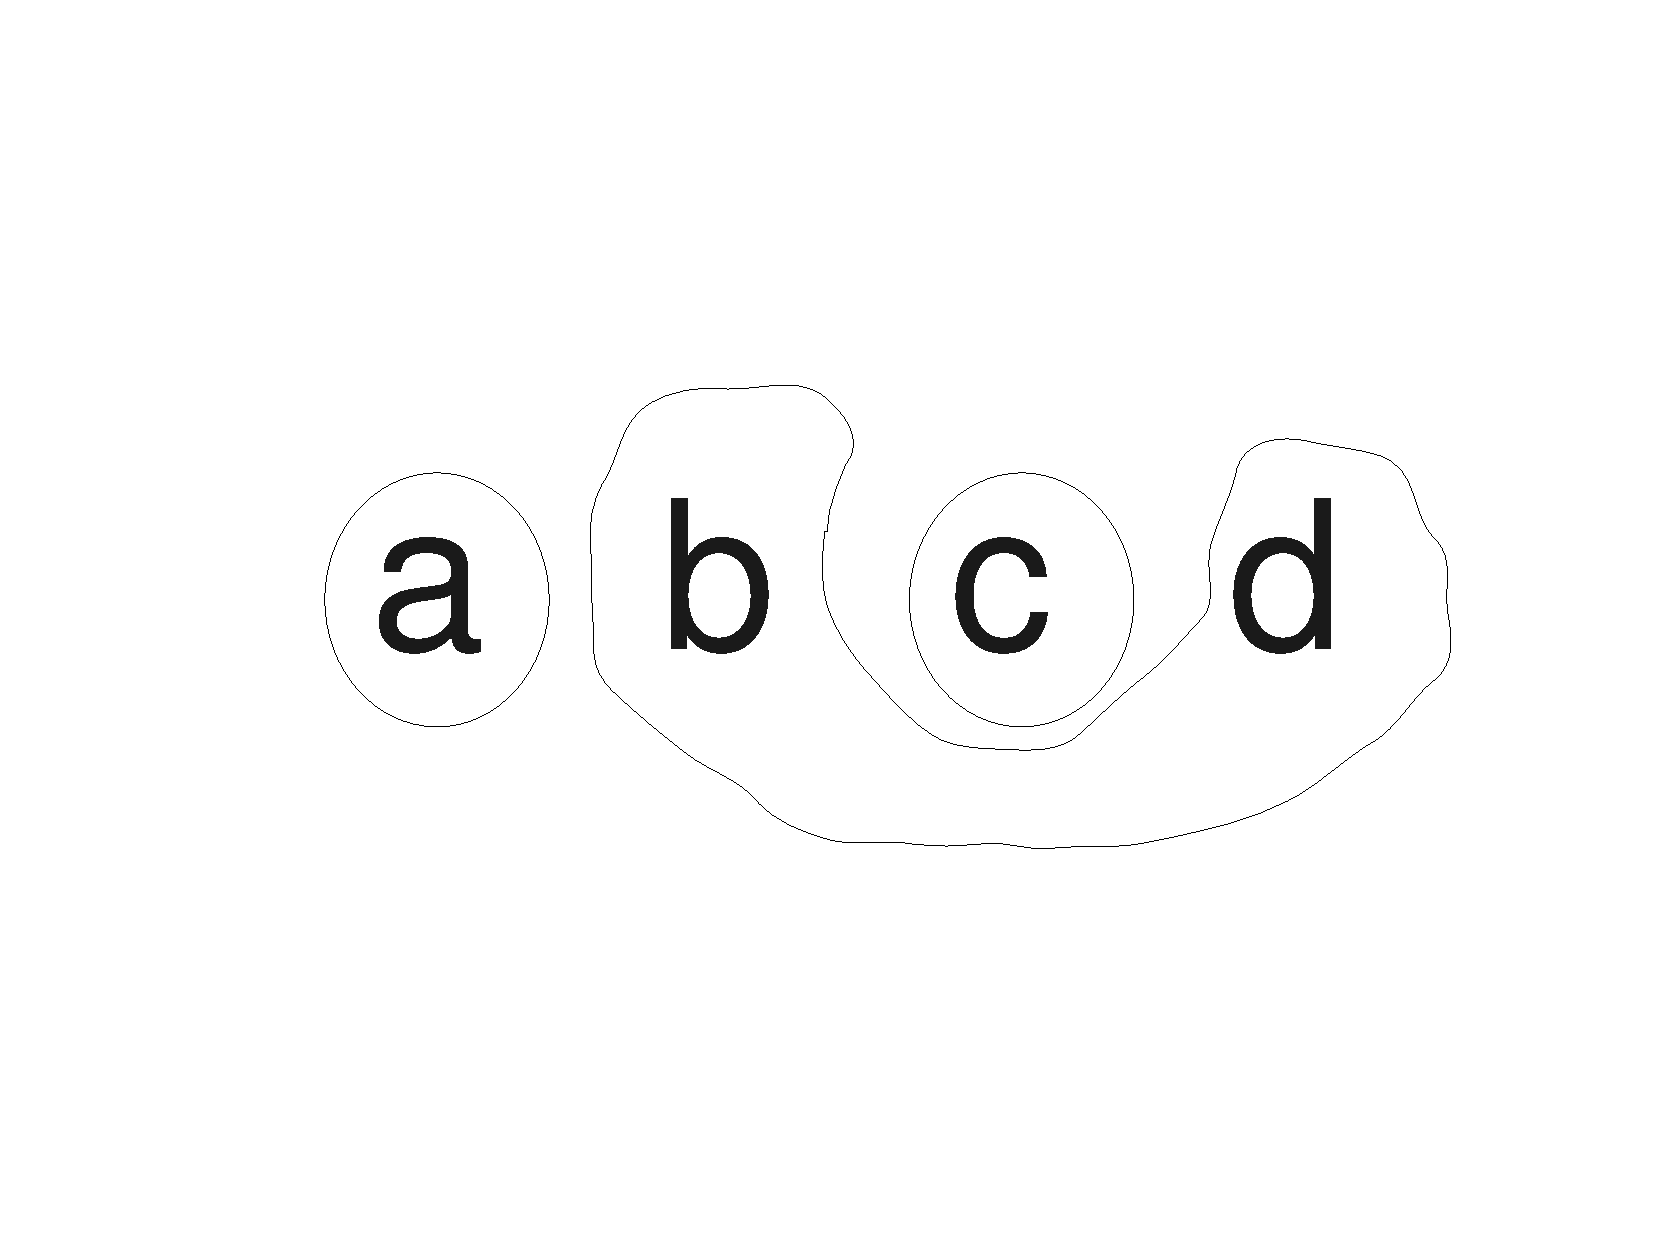
\includegraphics[width=0.5\textwidth]{fig/abcd3-2}
 \end{center}
 }
 
  \frame{\frametitle{}
 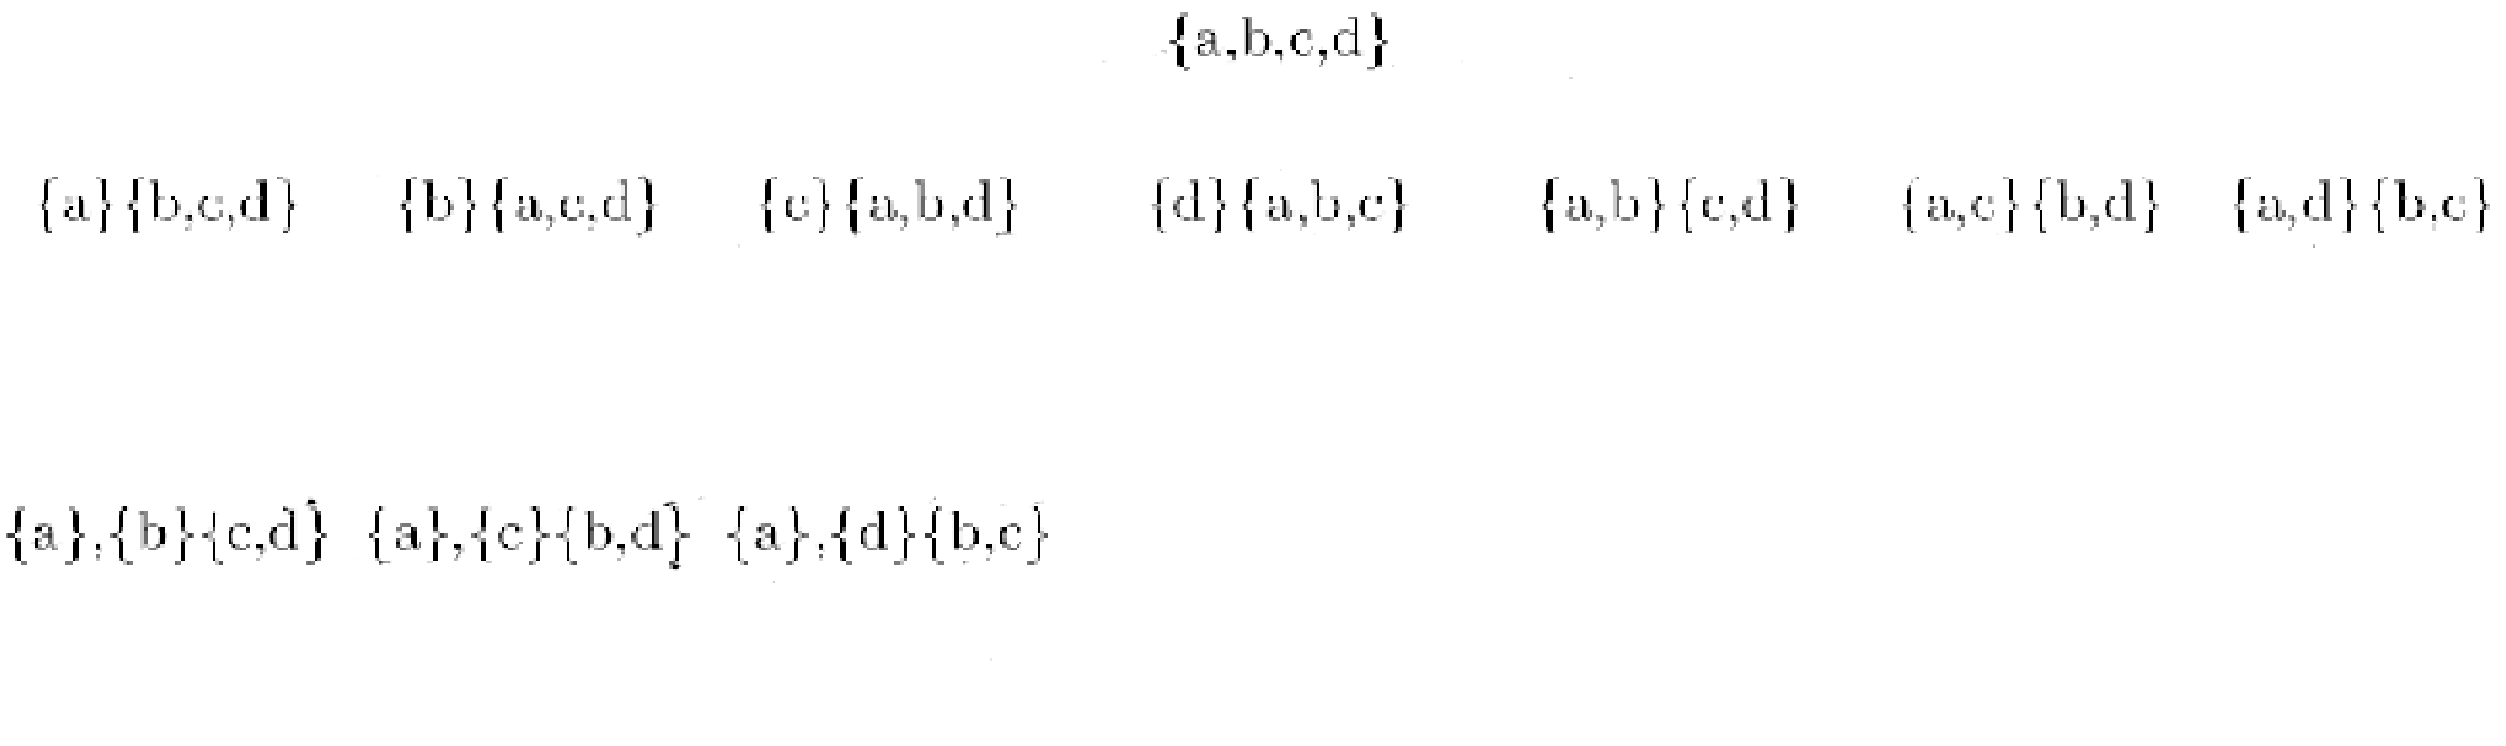
\includegraphics[width=\textwidth]{fig/part3-3}\\
 \begin{center}
 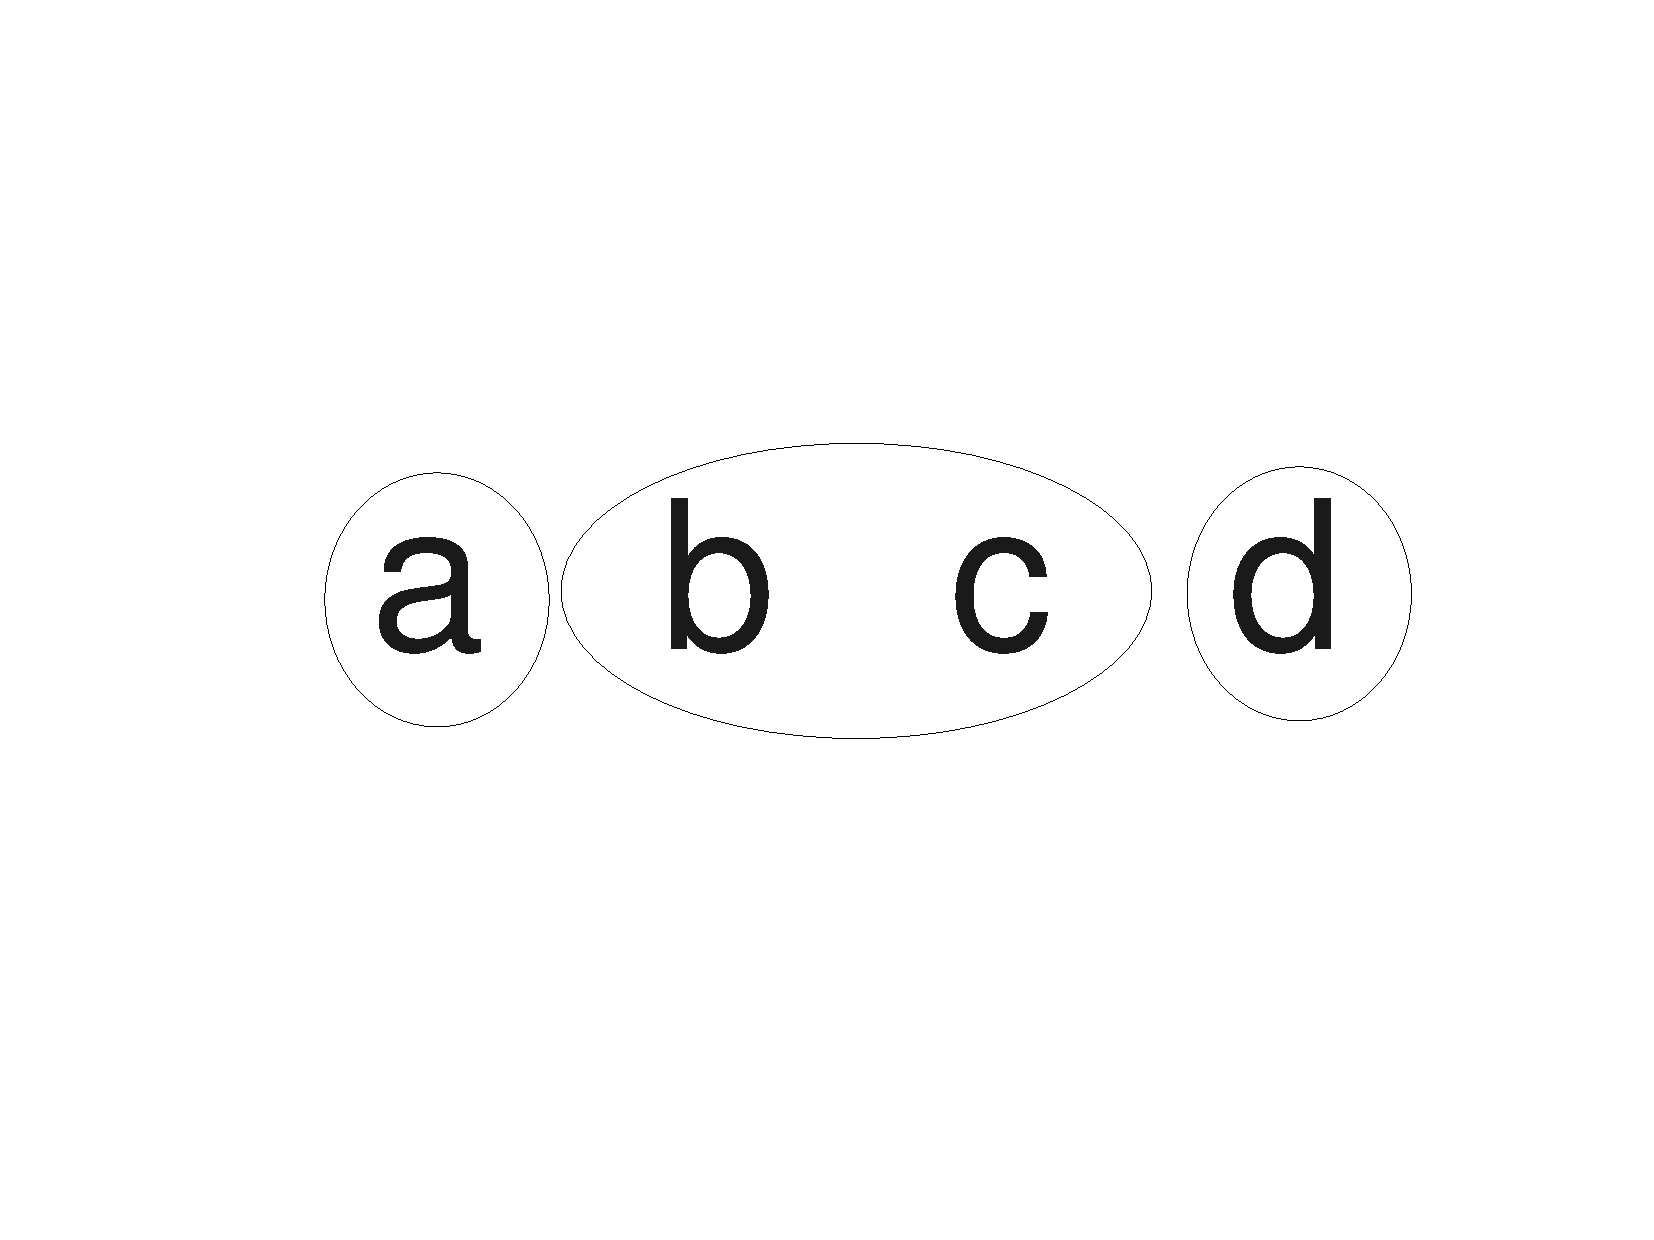
\includegraphics[width=0.5\textwidth]{fig/abcd3-3}
 \end{center}
 }
 
  \frame{\frametitle{}
 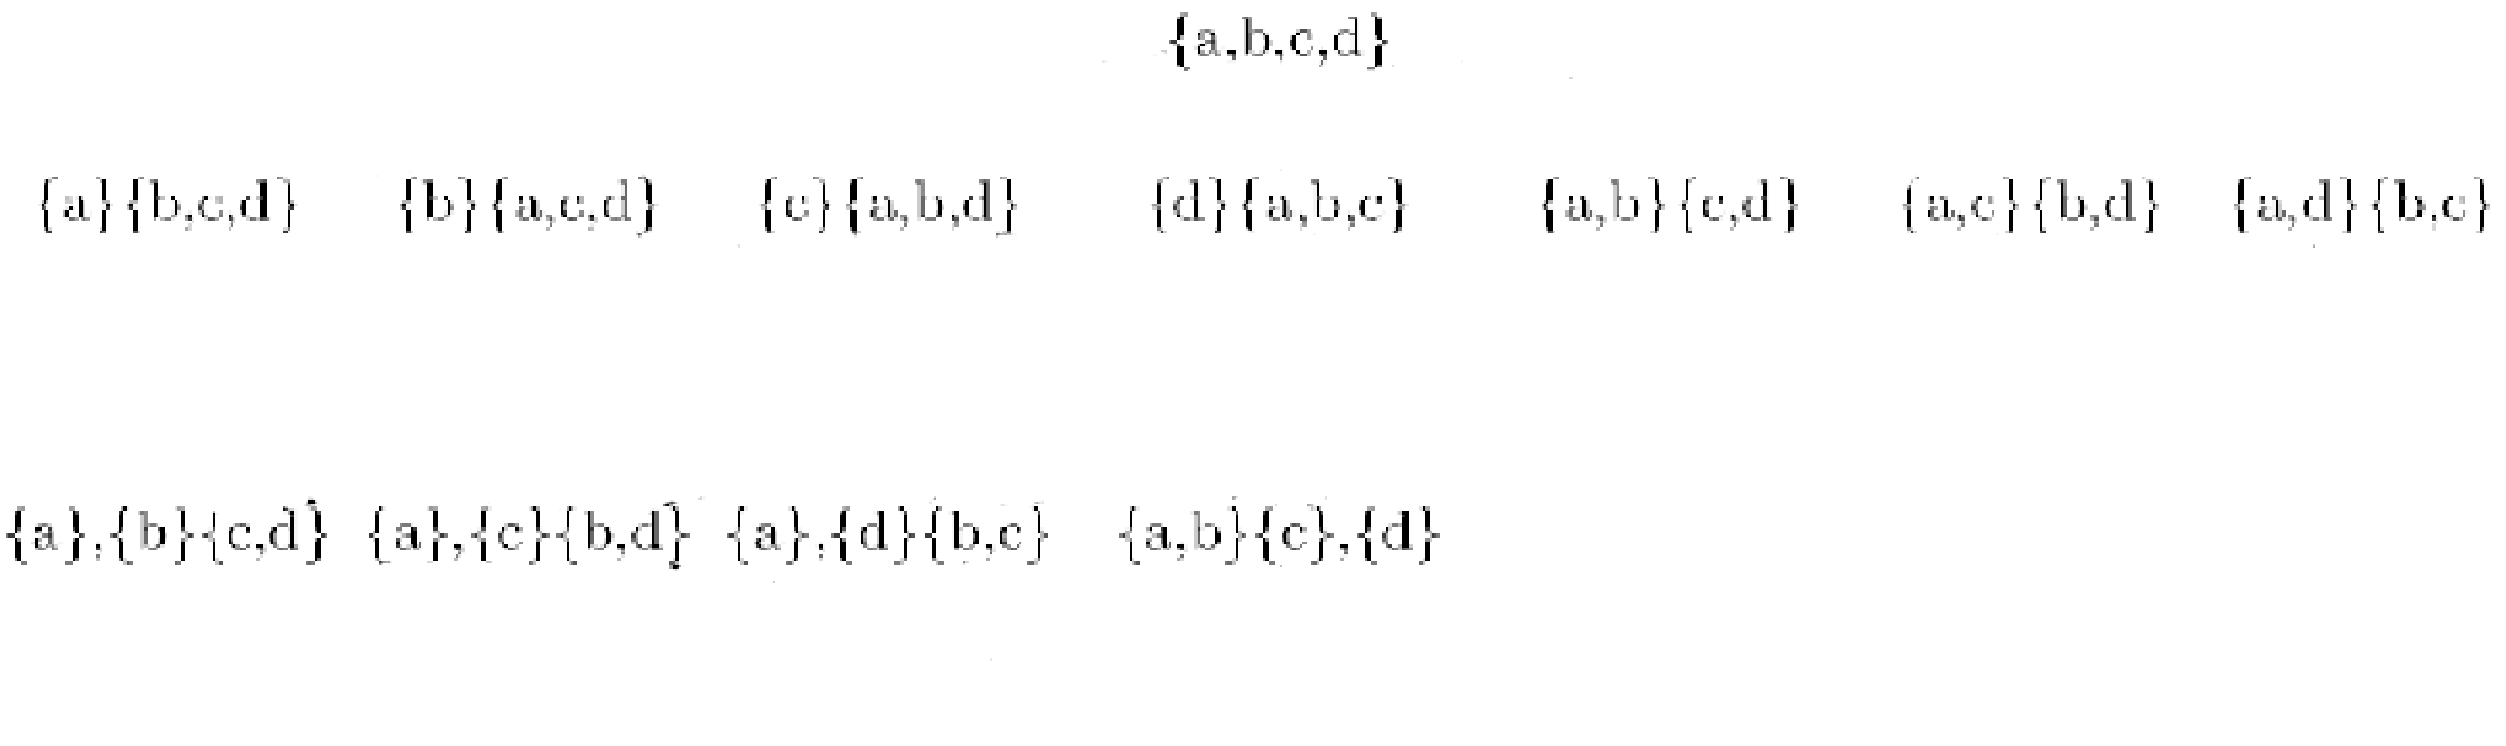
\includegraphics[width=\textwidth]{fig/part3-4}\\
 \begin{center}
 \includegraphics[width=0.5\textwidth]{fig/abcd3-4}
 \end{center}
 }
 
  \frame{\frametitle{}
 \includegraphics[width=\textwidth]{fig/part3-5}\\
 \begin{center}
 \includegraphics[width=0.5\textwidth]{fig/abcd3-5}
 \end{center}
 }
 
  \frame{\frametitle{}
 \includegraphics[width=\textwidth]{fig/part3-6}\\
 \begin{center}
 \includegraphics[width=0.5\textwidth]{fig/abcd3-6}
 \end{center}
 }
 
  \frame{\frametitle{}
 \includegraphics[width=\textwidth]{fig/part4-1}\\
 \begin{center}
 \includegraphics[width=0.5\textwidth]{fig/abcd4-1}
 \end{center}
 }
 
 
\frame{\frametitle{Merge Direction}
\includegraphics[width=\textwidth]{fig/hc_direction}
}


\frame{\frametitle{Example}
\includegraphics[width=0.9\textwidth]{fig/ahc_fig}
}


\frame{\frametitle{Example}
\includegraphics[width=0.9\textwidth]{fig/ahc_dendro}
}

\frame{\frametitle{Linkage}
\includegraphics[width=0.5\textwidth]{fig/linkage}
}


\frame{\frametitle{Zip Example: Cluster}
\includegraphics[width=0.9\textwidth]{fig/zip_cluster}
}

\frame{\frametitle{Zip Example: Classify}
\includegraphics[width=0.9\textwidth]{fig/zip_class}
}

\frame{\frametitle{Cat Example}
\includegraphics[width=0.9\textwidth]{fig/cat}
}

\frame{\frametitle{Cat Example}
\includegraphics[width=0.9\textwidth]{fig/cat_margin}
}

\frame{\frametitle{Cat Example}
\includegraphics[width=0.9\textwidth]{fig/cat_cluster}
}


\begin{frame}[fragile]\frametitle{}
\tiny	
\begin{lstlisting}
import numpy as np
import matplotlib.pylab as plt
%matplotlib inline
np.random.seed(0)
n = 100
X = np.vstack((np.random.multivariate_normal([0,0], [[1, 0], [0, 1]], n), 
             np.random.multivariate_normal([3, 3], [[1, 0], [0, 1]] , n)))
plt.scatter(X[:,0], X[:,1]);
\end{lstlisting} 

\begin{lstlisting}
import scipy.cluster.hierarchy as AHC
X_dist = AHC.distance.pdist(X) #make the pairwise distance
X_linkage = AHC.linkage(X_dist, method = "average")
den = AHC.dendrogram(X_linkage, no_labels = True)
\end{lstlisting} 

\begin{lstlisting}
from sklearn import cluster
X_kmeans = cluster.KMeans(n_clusters = 2)
X_kmeans.fit(X)
X_labels = X_kmeans.labels_
X_centers = X_kmeans.cluster_centers_
\end{lstlisting} 

\begin{lstlisting}
index=X_labels == 0 
plt.scatter(X[index, 0], X[index,1], color = "r")
plt.scatter(X[~index,0], X[~index,1], color = "b")
plt.scatter(X_centers[:,0], X_centers[:,1], color = "y", 
            facecolor="y", marker="+", s = 700)
\end{lstlisting} 
\end{frame}



%\begin{frame}[fragile]\frametitle{}
%\tiny	
%\begin{lstlisting}
%\end{lstlisting} 
%\end{frame}


%\begin{frame}[fragile]\frametitle{}
%\tiny	
%\begin{lstlisting}
%\end{lstlisting} 
%\end{frame}


%\frame{\frametitle{}
%\includegraphics[width=0.5\textwidth]{fig/}
%}

%\frame{\frametitle{}
%\includegraphics[width=0.5\textwidth]{fig/}
%}

%\frame{\frametitle{}
%\includegraphics[width=0.5\textwidth]{fig/}
%}
%
%
%
%

\end{document}
